\documentclass[a4paper]{book}
\usepackage{a4wide}
\usepackage{makeidx}
\usepackage{graphicx}
\usepackage{multicol}
\usepackage{float}
\usepackage{listings}
\usepackage{color}
\usepackage{textcomp}
\usepackage{alltt}
\usepackage{times}
\usepackage{ifpdf}
\ifpdf
\usepackage[pdftex,
            pagebackref=true,
            colorlinks=true,
            linkcolor=blue,
            unicode
           ]{hyperref}
\else
\usepackage[ps2pdf,
            pagebackref=true,
            colorlinks=true,
            linkcolor=blue,
            unicode
           ]{hyperref}
\usepackage{pspicture}
\fi
\usepackage[utf8]{inputenc}
\usepackage{doxygen}
\lstset{language=C++,inputencoding=utf8,basicstyle=\footnotesize,breaklines=true,breakatwhitespace=true,tabsize=8,numbers=left }
\makeindex
\setcounter{tocdepth}{3}
\renewcommand{\footrulewidth}{0.4pt}
\begin{document}
\hypersetup{pageanchor=false}
\begin{titlepage}
\vspace*{7cm}
\begin{center}
{\Large Brick Breaker \\[1ex]\large 3.1.4 }\\
\vspace*{1cm}
{\large Generated by Doxygen 1.6.3}\\
\vspace*{0.5cm}
{\small Tue May 4 15:09:18 2010}\\
\end{center}
\end{titlepage}
\clearemptydoublepage
\pagenumbering{roman}
\tableofcontents
\clearemptydoublepage
\pagenumbering{arabic}
\hypersetup{pageanchor=true}
\chapter{Class Index}
\section{Class Hierarchy}
This inheritance list is sorted roughly, but not completely, alphabetically:\begin{DoxyCompactList}
\item \contentsline{section}{brickBreaker.Ball}{\pageref{classbrick_breaker_1_1_ball}}{}
\item \contentsline{section}{brickBreaker.Brick}{\pageref{classbrick_breaker_1_1_brick}}{}
\begin{DoxyCompactList}
\item \contentsline{section}{brickBreaker.PermanentBrick}{\pageref{classbrick_breaker_1_1_permanent_brick}}{}
\item \contentsline{section}{brickBreaker.StandardBrick}{\pageref{classbrick_breaker_1_1_standard_brick}}{}
\begin{DoxyCompactList}
\item \contentsline{section}{brickBreaker.PowerBrick}{\pageref{classbrick_breaker_1_1_power_brick}}{}
\end{DoxyCompactList}
\end{DoxyCompactList}
\item \contentsline{section}{brickBreaker.web.ConnectionUtil}{\pageref{classbrick_breaker_1_1web_1_1_connection_util}}{}
\item \contentsline{section}{brickBreaker.web.EncryptionFailureException}{\pageref{classbrick_breaker_1_1web_1_1_encryption_failure_exception}}{}
\item \contentsline{section}{brickBreaker.web.EncryptionUtil}{\pageref{classbrick_breaker_1_1web_1_1_encryption_util}}{}
\item \contentsline{section}{brickBreaker.local.FilesystemFailureException}{\pageref{classbrick_breaker_1_1local_1_1_filesystem_failure_exception}}{}
\item \contentsline{section}{brickBreaker.web.HighScore}{\pageref{classbrick_breaker_1_1web_1_1_high_score}}{}
\item \contentsline{section}{brickBreaker.web.InvalidUserException}{\pageref{classbrick_breaker_1_1web_1_1_invalid_user_exception}}{}
\item \contentsline{section}{brickBreaker.Level}{\pageref{classbrick_breaker_1_1_level}}{}
\item \contentsline{section}{brickBreaker.local.LevelCatalog}{\pageref{classbrick_breaker_1_1local_1_1_level_catalog}}{}
\item \contentsline{section}{brickBreaker.LevelInitializer}{\pageref{classbrick_breaker_1_1_level_initializer}}{}
\item \contentsline{section}{brickBreaker.LevelPlayer}{\pageref{classbrick_breaker_1_1_level_player}}{}
\item \contentsline{section}{brickBreaker.local.LocalDataService}{\pageref{classbrick_breaker_1_1local_1_1_local_data_service}}{}
\item \contentsline{section}{brickBreaker.web.OnlineLevel}{\pageref{classbrick_breaker_1_1web_1_1_online_level}}{}
\item \contentsline{section}{brickBreaker.PasswordBox}{\pageref{classbrick_breaker_1_1_password_box}}{}
\item \contentsline{section}{brickBreaker.PRPanel}{\pageref{classbrick_breaker_1_1_p_r_panel}}{}
\begin{DoxyCompactList}
\item \contentsline{section}{brickBreaker.GamePanel}{\pageref{classbrick_breaker_1_1_game_panel}}{}
\item \contentsline{section}{brickBreaker.IdlePanel}{\pageref{classbrick_breaker_1_1_idle_panel}}{}
\item \contentsline{section}{brickBreaker.LevelEditor}{\pageref{classbrick_breaker_1_1_level_editor}}{}
\end{DoxyCompactList}
\item \contentsline{section}{brickBreaker.Racket}{\pageref{classbrick_breaker_1_1_racket}}{}
\begin{DoxyCompactList}
\item \contentsline{section}{brickBreaker.HorizontalRacket}{\pageref{classbrick_breaker_1_1_horizontal_racket}}{}
\item \contentsline{section}{brickBreaker.VerticalRacket}{\pageref{classbrick_breaker_1_1_vertical_racket}}{}
\end{DoxyCompactList}
\item \contentsline{section}{brickBreaker.web.RequestFailureException}{\pageref{classbrick_breaker_1_1web_1_1_request_failure_exception}}{}
\item \contentsline{section}{brickBreaker.Start}{\pageref{classbrick_breaker_1_1_start}}{}
\item \contentsline{section}{brickBreaker.StartEditor}{\pageref{classbrick_breaker_1_1_start_editor}}{}
\item \contentsline{section}{brickBreaker.StartIdle}{\pageref{classbrick_breaker_1_1_start_idle}}{}
\item \contentsline{section}{brickBreaker.web.UserConfig}{\pageref{classbrick_breaker_1_1web_1_1_user_config}}{}
\item \contentsline{section}{brickBreaker.web.WebConfig}{\pageref{classbrick_breaker_1_1web_1_1_web_config}}{}
\item \contentsline{section}{brickBreaker.web.WebException}{\pageref{classbrick_breaker_1_1web_1_1_web_exception}}{}
\item \contentsline{section}{brickBreaker.web.WebService}{\pageref{classbrick_breaker_1_1web_1_1_web_service}}{}
\item \contentsline{section}{brickBreaker.web.XMLParseFailureException}{\pageref{classbrick_breaker_1_1web_1_1_x_m_l_parse_failure_exception}}{}
\item \contentsline{section}{brickBreaker.web.XMLUtil}{\pageref{classbrick_breaker_1_1web_1_1_x_m_l_util}}{}
\end{DoxyCompactList}

\chapter{Class Index}
\section{Data Structures}
Here are the data structures with brief descriptions:\begin{DoxyCompactList}
\item\contentsline{section}{\hyperlink{class_blob}{Blob} }{\pageref{class_blob}}{}
\item\contentsline{section}{\hyperlink{class_blobs_controller}{BlobsController} }{\pageref{class_blobs_controller}}{}
\item\contentsline{section}{\hyperlink{class_d_a_t_a_b_a_s_e___c_o_n_f_i_g}{DATABASE\_\-CONFIG} }{\pageref{class_d_a_t_a_b_a_s_e___c_o_n_f_i_g}}{}
\item\contentsline{section}{\hyperlink{class_db_acl_schema}{DbAclSchema} }{\pageref{class_db_acl_schema}}{}
\item\contentsline{section}{\hyperlink{classi18n_schema}{i18nSchema} }{\pageref{classi18n_schema}}{}
\item\contentsline{section}{\hyperlink{class_score}{Score} }{\pageref{class_score}}{}
\item\contentsline{section}{\hyperlink{class_scores_controller}{ScoresController} }{\pageref{class_scores_controller}}{}
\item\contentsline{section}{\hyperlink{class_sessions_schema}{SessionsSchema} }{\pageref{class_sessions_schema}}{}
\item\contentsline{section}{\hyperlink{class_user}{User} }{\pageref{class_user}}{}
\item\contentsline{section}{\hyperlink{class_users_controller}{UsersController} }{\pageref{class_users_controller}}{}
\end{DoxyCompactList}

\chapter{File Index}
\section{File List}
Here is a list of all documented files with brief descriptions:\begin{DoxyCompactList}
\item\contentsline{section}{src/game/brickBreaker/\hyperlink{_ball_8java}{Ball.java} }{\pageref{_ball_8java}}{}
\item\contentsline{section}{src/game/brickBreaker/\hyperlink{_brick_8java}{Brick.java} }{\pageref{_brick_8java}}{}
\item\contentsline{section}{src/game/brickBreaker/\hyperlink{_game_panel_8java}{GamePanel.java} }{\pageref{_game_panel_8java}}{}
\item\contentsline{section}{src/game/brickBreaker/\hyperlink{_horizontal_racket_8java}{HorizontalRacket.java} }{\pageref{_horizontal_racket_8java}}{}
\item\contentsline{section}{src/game/brickBreaker/\hyperlink{_idle_panel_8java}{IdlePanel.java} }{\pageref{_idle_panel_8java}}{}
\item\contentsline{section}{src/game/brickBreaker/\hyperlink{_level_8java}{Level.java} }{\pageref{_level_8java}}{}
\item\contentsline{section}{src/game/brickBreaker/\hyperlink{_level_player_8java}{LevelPlayer.java} }{\pageref{_level_player_8java}}{}
\item\contentsline{section}{src/game/brickBreaker/\hyperlink{_password_box_8java}{PasswordBox.java} }{\pageref{_password_box_8java}}{}
\item\contentsline{section}{src/game/brickBreaker/\hyperlink{_permanent_brick_8java}{PermanentBrick.java} }{\pageref{_permanent_brick_8java}}{}
\item\contentsline{section}{src/game/brickBreaker/\hyperlink{_power_brick_8java}{PowerBrick.java} }{\pageref{_power_brick_8java}}{}
\item\contentsline{section}{src/game/brickBreaker/\hyperlink{_p_r_panel_8java}{PRPanel.java} }{\pageref{_p_r_panel_8java}}{}
\item\contentsline{section}{src/game/brickBreaker/\hyperlink{_racket_8java}{Racket.java} }{\pageref{_racket_8java}}{}
\item\contentsline{section}{src/game/brickBreaker/\hyperlink{_standard_brick_8java}{StandardBrick.java} }{\pageref{_standard_brick_8java}}{}
\item\contentsline{section}{src/game/brickBreaker/\hyperlink{_start_8java}{Start.java} }{\pageref{_start_8java}}{}
\item\contentsline{section}{src/game/brickBreaker/\hyperlink{_vertical_racket_8java}{VerticalRacket.java} }{\pageref{_vertical_racket_8java}}{}
\end{DoxyCompactList}

\chapter{Class Documentation}
\hypertarget{classbrick_breaker_1_1_ball}{
\section{brickBreaker.Ball Class Reference}
\label{classbrick_breaker_1_1_ball}\index{brickBreaker::Ball@{brickBreaker::Ball}}
}


Inherits java::io::Serializable.

\subsection*{Public Member Functions}
\begin{DoxyCompactItemize}
\item 
\hyperlink{classbrick_breaker_1_1_ball_acb18370d945b133d9c3a3d87beca7e4c}{Ball} (\hyperlink{classbrick_breaker_1_1_racket}{Racket}\mbox{[}$\,$\mbox{]} r, int radius)
\item 
\hyperlink{classbrick_breaker_1_1_ball_ae797eeb30e776dbe48357107816db887}{Ball} (\hyperlink{classbrick_breaker_1_1_level_player}{LevelPlayer} l, \hyperlink{classbrick_breaker_1_1_racket}{Racket}\mbox{[}$\,$\mbox{]} r, int radius)
\item 
void \hyperlink{classbrick_breaker_1_1_ball_adcc8436d899828fe7f3c788ed1daf8d6}{setLoc} (double x, double y, double angle)
\item 
void \hyperlink{classbrick_breaker_1_1_ball_a3a95a5d7eeab58dbacd89d1e304bf2d4}{setLevel} (\hyperlink{classbrick_breaker_1_1_level_player}{LevelPlayer} lev)
\item 
int \hyperlink{classbrick_breaker_1_1_ball_a7c119360e2434ef5c69020e8608569ff}{updatePosition} ()
\item 
void \hyperlink{classbrick_breaker_1_1_ball_ab2ed912dfac55974d85184840fd8be9d}{draw} (Graphics g)
\item 
int \hyperlink{classbrick_breaker_1_1_ball_af0651b3d0294b6843a7a5b74acb87195}{getX} ()
\item 
int \hyperlink{classbrick_breaker_1_1_ball_abc92d446c039bfae85f89ba82facdfc3}{getY} ()
\item 
int \hyperlink{classbrick_breaker_1_1_ball_ae4ca4fc89a298a422b96c3056e9b9d1a}{getRad} ()
\item 
void \hyperlink{classbrick_breaker_1_1_ball_a71e24748f9cb90bd9da6a910648ba84e}{setX} (double x)
\item 
void \hyperlink{classbrick_breaker_1_1_ball_ae15aedc6cd01476f486328369fd6a799}{setY} (double y)
\item 
boolean \hyperlink{classbrick_breaker_1_1_ball_ac516403ca5285c41619248f6c1e0690b}{inBounds} ()
\item 
void \hyperlink{classbrick_breaker_1_1_ball_a443ce0341305785eaf4da97d755bb550}{changeAngle} (double newAngle)
\item 
double \hyperlink{classbrick_breaker_1_1_ball_a022f1feac935da4a1480fc70f56858d4}{getAngle} ()
\item 
boolean \hyperlink{classbrick_breaker_1_1_ball_aff35873f2550b5b0601cfb7b31cfc368}{checkCollision} (int\mbox{[}$\,$\mbox{]} loc)
\item 
void \hyperlink{classbrick_breaker_1_1_ball_a102b54397819a72161278ccfeb1f5d72}{bounce} (int x, boolean horizontal)
\end{DoxyCompactItemize}
\subsection*{Static Public Member Functions}
\begin{DoxyCompactItemize}
\item 
static void \hyperlink{classbrick_breaker_1_1_ball_ad43ce78383f0415e608cb247e5df9ecd}{resetVars} ()
\end{DoxyCompactItemize}
\subsection*{Static Public Attributes}
\begin{DoxyCompactItemize}
\item 
\hypertarget{classbrick_breaker_1_1_ball_a982ccc918368e8e543cd60c79906b23b}{
static final double {\bfseries pi} = Math.PI}
\label{classbrick_breaker_1_1_ball_a982ccc918368e8e543cd60c79906b23b}

\item 
\hypertarget{classbrick_breaker_1_1_ball_a823ecce6d62f6f51d6295e10a02ecb96}{
static double {\bfseries speed}}
\label{classbrick_breaker_1_1_ball_a823ecce6d62f6f51d6295e10a02ecb96}

\item 
\hypertarget{classbrick_breaker_1_1_ball_a9dac0bf349181dcee6b23afc37651064}{
static int {\bfseries powerLevel} = 0}
\label{classbrick_breaker_1_1_ball_a9dac0bf349181dcee6b23afc37651064}

\item 
\hypertarget{classbrick_breaker_1_1_ball_a9bad3add0bff004075b750e2f7cf35f4}{
static double {\bfseries ptMultiplier} = 1}
\label{classbrick_breaker_1_1_ball_a9bad3add0bff004075b750e2f7cf35f4}

\end{DoxyCompactItemize}


\subsection{Constructor \& Destructor Documentation}
\hypertarget{classbrick_breaker_1_1_ball_acb18370d945b133d9c3a3d87beca7e4c}{
\index{brickBreaker::Ball@{brickBreaker::Ball}!Ball@{Ball}}
\index{Ball@{Ball}!brickBreaker::Ball@{brickBreaker::Ball}}
\subsubsection[{Ball}]{\setlength{\rightskip}{0pt plus 5cm}brickBreaker.Ball.Ball ({\bf Racket}\mbox{[}$\,$\mbox{]} {\em r}, \/  int {\em radius})}}
\label{classbrick_breaker_1_1_ball_acb18370d945b133d9c3a3d87beca7e4c}
Constructor.


\begin{DoxyParams}{Parameters}
\item[{\em r}]An array of all rackets in the game \item[{\em radius}]The radius of the ball, in pixels \end{DoxyParams}
\hypertarget{classbrick_breaker_1_1_ball_ae797eeb30e776dbe48357107816db887}{
\index{brickBreaker::Ball@{brickBreaker::Ball}!Ball@{Ball}}
\index{Ball@{Ball}!brickBreaker::Ball@{brickBreaker::Ball}}
\subsubsection[{Ball}]{\setlength{\rightskip}{0pt plus 5cm}brickBreaker.Ball.Ball ({\bf LevelPlayer} {\em l}, \/  {\bf Racket}\mbox{[}$\,$\mbox{]} {\em r}, \/  int {\em radius})}}
\label{classbrick_breaker_1_1_ball_ae797eeb30e776dbe48357107816db887}
Constructor.


\begin{DoxyParams}{Parameters}
\item[{\em l}]The \hyperlink{classbrick_breaker_1_1_level_player}{LevelPlayer} in which the ball exists \item[{\em r}]An array of all rackets in the game \item[{\em radius}]The radius of the ball, in pixels \end{DoxyParams}


\subsection{Member Function Documentation}
\hypertarget{classbrick_breaker_1_1_ball_a102b54397819a72161278ccfeb1f5d72}{
\index{brickBreaker::Ball@{brickBreaker::Ball}!bounce@{bounce}}
\index{bounce@{bounce}!brickBreaker::Ball@{brickBreaker::Ball}}
\subsubsection[{bounce}]{\setlength{\rightskip}{0pt plus 5cm}void brickBreaker.Ball.bounce (int {\em x}, \/  boolean {\em horizontal})}}
\label{classbrick_breaker_1_1_ball_a102b54397819a72161278ccfeb1f5d72}
Bounces this ball off the given wall. The wall is either horizontal or vertical, specified by param horizontal. 
\begin{DoxyParams}{Parameters}
\item[{\em x}]The location of the wall \item[{\em horizontal}]True if the wall is horizontal, false if it is vertical \end{DoxyParams}
\hypertarget{classbrick_breaker_1_1_ball_a443ce0341305785eaf4da97d755bb550}{
\index{brickBreaker::Ball@{brickBreaker::Ball}!changeAngle@{changeAngle}}
\index{changeAngle@{changeAngle}!brickBreaker::Ball@{brickBreaker::Ball}}
\subsubsection[{changeAngle}]{\setlength{\rightskip}{0pt plus 5cm}void brickBreaker.Ball.changeAngle (double {\em newAngle})}}
\label{classbrick_breaker_1_1_ball_a443ce0341305785eaf4da97d755bb550}
Changes the ball's angle to the new value. 
\begin{DoxyParams}{Parameters}
\item[{\em newAngle}]The new angle \end{DoxyParams}
\hypertarget{classbrick_breaker_1_1_ball_aff35873f2550b5b0601cfb7b31cfc368}{
\index{brickBreaker::Ball@{brickBreaker::Ball}!checkCollision@{checkCollision}}
\index{checkCollision@{checkCollision}!brickBreaker::Ball@{brickBreaker::Ball}}
\subsubsection[{checkCollision}]{\setlength{\rightskip}{0pt plus 5cm}boolean brickBreaker.Ball.checkCollision (int\mbox{[}$\,$\mbox{]} {\em loc})}}
\label{classbrick_breaker_1_1_ball_aff35873f2550b5b0601cfb7b31cfc368}
Checks if the ball is colliding with the given object If a collision exists and changeDir is true, it changes the ball's direction


\begin{DoxyParams}{Parameters}
\item[{\em loc}]A block to be tested, represented by an int array containing, in order, x, y, width and height of the brick \end{DoxyParams}
\begin{DoxyReturn}{Returns}
Returns true if the ball hit the object, false if not 
\end{DoxyReturn}
\hypertarget{classbrick_breaker_1_1_ball_ab2ed912dfac55974d85184840fd8be9d}{
\index{brickBreaker::Ball@{brickBreaker::Ball}!draw@{draw}}
\index{draw@{draw}!brickBreaker::Ball@{brickBreaker::Ball}}
\subsubsection[{draw}]{\setlength{\rightskip}{0pt plus 5cm}void brickBreaker.Ball.draw (Graphics {\em g})}}
\label{classbrick_breaker_1_1_ball_ab2ed912dfac55974d85184840fd8be9d}
Draws the ball on the screen.


\begin{DoxyParams}{Parameters}
\item[{\em g}]The graphics object with which to draw \end{DoxyParams}
\hypertarget{classbrick_breaker_1_1_ball_a022f1feac935da4a1480fc70f56858d4}{
\index{brickBreaker::Ball@{brickBreaker::Ball}!getAngle@{getAngle}}
\index{getAngle@{getAngle}!brickBreaker::Ball@{brickBreaker::Ball}}
\subsubsection[{getAngle}]{\setlength{\rightskip}{0pt plus 5cm}double brickBreaker.Ball.getAngle ()}}
\label{classbrick_breaker_1_1_ball_a022f1feac935da4a1480fc70f56858d4}
Returns the ball's current angle. \hypertarget{classbrick_breaker_1_1_ball_ae4ca4fc89a298a422b96c3056e9b9d1a}{
\index{brickBreaker::Ball@{brickBreaker::Ball}!getRad@{getRad}}
\index{getRad@{getRad}!brickBreaker::Ball@{brickBreaker::Ball}}
\subsubsection[{getRad}]{\setlength{\rightskip}{0pt plus 5cm}int brickBreaker.Ball.getRad ()}}
\label{classbrick_breaker_1_1_ball_ae4ca4fc89a298a422b96c3056e9b9d1a}
\begin{DoxyReturn}{Returns}
Returns the ball's radius, in pixels 
\end{DoxyReturn}
\hypertarget{classbrick_breaker_1_1_ball_af0651b3d0294b6843a7a5b74acb87195}{
\index{brickBreaker::Ball@{brickBreaker::Ball}!getX@{getX}}
\index{getX@{getX}!brickBreaker::Ball@{brickBreaker::Ball}}
\subsubsection[{getX}]{\setlength{\rightskip}{0pt plus 5cm}int brickBreaker.Ball.getX ()}}
\label{classbrick_breaker_1_1_ball_af0651b3d0294b6843a7a5b74acb87195}
\begin{DoxyReturn}{Returns}
Returns the current x-\/coordinate, rounded to the nearest int 
\end{DoxyReturn}
\hypertarget{classbrick_breaker_1_1_ball_abc92d446c039bfae85f89ba82facdfc3}{
\index{brickBreaker::Ball@{brickBreaker::Ball}!getY@{getY}}
\index{getY@{getY}!brickBreaker::Ball@{brickBreaker::Ball}}
\subsubsection[{getY}]{\setlength{\rightskip}{0pt plus 5cm}int brickBreaker.Ball.getY ()}}
\label{classbrick_breaker_1_1_ball_abc92d446c039bfae85f89ba82facdfc3}
\begin{DoxyReturn}{Returns}
Returns the current y-\/coordinate, rounded to the nearest int 
\end{DoxyReturn}
\hypertarget{classbrick_breaker_1_1_ball_ac516403ca5285c41619248f6c1e0690b}{
\index{brickBreaker::Ball@{brickBreaker::Ball}!inBounds@{inBounds}}
\index{inBounds@{inBounds}!brickBreaker::Ball@{brickBreaker::Ball}}
\subsubsection[{inBounds}]{\setlength{\rightskip}{0pt plus 5cm}boolean brickBreaker.Ball.inBounds ()}}
\label{classbrick_breaker_1_1_ball_ac516403ca5285c41619248f6c1e0690b}
\begin{DoxyReturn}{Returns}
Returns true if the ball is still in play 
\end{DoxyReturn}
\hypertarget{classbrick_breaker_1_1_ball_ad43ce78383f0415e608cb247e5df9ecd}{
\index{brickBreaker::Ball@{brickBreaker::Ball}!resetVars@{resetVars}}
\index{resetVars@{resetVars}!brickBreaker::Ball@{brickBreaker::Ball}}
\subsubsection[{resetVars}]{\setlength{\rightskip}{0pt plus 5cm}static void brickBreaker.Ball.resetVars ()\hspace{0.3cm}{\ttfamily  \mbox{[}static\mbox{]}}}}
\label{classbrick_breaker_1_1_ball_ad43ce78383f0415e608cb247e5df9ecd}
Resets all the static variables in this class to their initial values. \hypertarget{classbrick_breaker_1_1_ball_a3a95a5d7eeab58dbacd89d1e304bf2d4}{
\index{brickBreaker::Ball@{brickBreaker::Ball}!setLevel@{setLevel}}
\index{setLevel@{setLevel}!brickBreaker::Ball@{brickBreaker::Ball}}
\subsubsection[{setLevel}]{\setlength{\rightskip}{0pt plus 5cm}void brickBreaker.Ball.setLevel ({\bf LevelPlayer} {\em lev})}}
\label{classbrick_breaker_1_1_ball_a3a95a5d7eeab58dbacd89d1e304bf2d4}
Changes the \hyperlink{classbrick_breaker_1_1_level_player}{LevelPlayer} in which the ball exists. Usually called after the first constructor, in which the \hyperlink{classbrick_breaker_1_1_level_player}{LevelPlayer} is not specified.


\begin{DoxyParams}{Parameters}
\item[{\em lev}]New \hyperlink{classbrick_breaker_1_1_level_player}{LevelPlayer} \end{DoxyParams}
\hypertarget{classbrick_breaker_1_1_ball_adcc8436d899828fe7f3c788ed1daf8d6}{
\index{brickBreaker::Ball@{brickBreaker::Ball}!setLoc@{setLoc}}
\index{setLoc@{setLoc}!brickBreaker::Ball@{brickBreaker::Ball}}
\subsubsection[{setLoc}]{\setlength{\rightskip}{0pt plus 5cm}void brickBreaker.Ball.setLoc (double {\em x}, \/  double {\em y}, \/  double {\em angle})}}
\label{classbrick_breaker_1_1_ball_adcc8436d899828fe7f3c788ed1daf8d6}
Sets the ball's location and direction to the given coordinates.


\begin{DoxyParams}{Parameters}
\item[{\em x}]New x-\/coordinate \item[{\em y}]New y-\/coordinate \item[{\em angle}]New Angle \end{DoxyParams}
\hypertarget{classbrick_breaker_1_1_ball_a71e24748f9cb90bd9da6a910648ba84e}{
\index{brickBreaker::Ball@{brickBreaker::Ball}!setX@{setX}}
\index{setX@{setX}!brickBreaker::Ball@{brickBreaker::Ball}}
\subsubsection[{setX}]{\setlength{\rightskip}{0pt plus 5cm}void brickBreaker.Ball.setX (double {\em x})}}
\label{classbrick_breaker_1_1_ball_a71e24748f9cb90bd9da6a910648ba84e}
Sets the x-\/coordinate to the new value. 
\begin{DoxyParams}{Parameters}
\item[{\em x}]The new x-\/coordinate \end{DoxyParams}
\hypertarget{classbrick_breaker_1_1_ball_ae15aedc6cd01476f486328369fd6a799}{
\index{brickBreaker::Ball@{brickBreaker::Ball}!setY@{setY}}
\index{setY@{setY}!brickBreaker::Ball@{brickBreaker::Ball}}
\subsubsection[{setY}]{\setlength{\rightskip}{0pt plus 5cm}void brickBreaker.Ball.setY (double {\em y})}}
\label{classbrick_breaker_1_1_ball_ae15aedc6cd01476f486328369fd6a799}
Sets the y-\/coordinate to the new value. 
\begin{DoxyParams}{Parameters}
\item[{\em y}]The new y-\/coordinate \end{DoxyParams}
\hypertarget{classbrick_breaker_1_1_ball_a7c119360e2434ef5c69020e8608569ff}{
\index{brickBreaker::Ball@{brickBreaker::Ball}!updatePosition@{updatePosition}}
\index{updatePosition@{updatePosition}!brickBreaker::Ball@{brickBreaker::Ball}}
\subsubsection[{updatePosition}]{\setlength{\rightskip}{0pt plus 5cm}int brickBreaker.Ball.updatePosition ()}}
\label{classbrick_breaker_1_1_ball_a7c119360e2434ef5c69020e8608569ff}
Updates the position of the ball and calculates the number of points earned.

\begin{DoxyReturn}{Returns}
Returns the number of points earned during this time step. 
\end{DoxyReturn}


The documentation for this class was generated from the following file:\begin{DoxyCompactItemize}
\item 
src/game/brickBreaker/\hyperlink{_ball_8java}{Ball.java}\end{DoxyCompactItemize}

\hypertarget{classbrick_breaker_1_1_brick}{
\section{brickBreaker.Brick Class Reference}
\label{classbrick_breaker_1_1_brick}\index{brickBreaker::Brick@{brickBreaker::Brick}}
}
Inheritance diagram for brickBreaker.Brick:\begin{figure}[H]
\begin{center}
\leavevmode
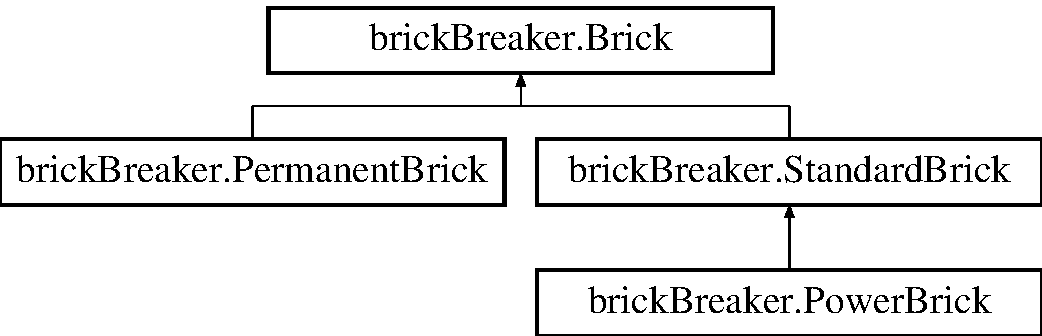
\includegraphics[height=3cm]{classbrick_breaker_1_1_brick}
\end{center}
\end{figure}
\subsection*{Public Member Functions}
\begin{DoxyCompactItemize}
\item 
\hyperlink{classbrick_breaker_1_1_brick_a48498f7c136cce1f0742ec4406ac2831}{Brick} (int pts, int hits, Color c)
\item 
void \hyperlink{classbrick_breaker_1_1_brick_a6f9ff21504eab68a2b9b9e6a87ed0f52}{setLoc} (int x, int y, int wid, int hgt)
\item 
int \hyperlink{classbrick_breaker_1_1_brick_a8b7ce8ba47ffe6de06c0c6121cdaa231}{bounce} (\hyperlink{classbrick_breaker_1_1_ball}{Ball} ball)
\item 
boolean \hyperlink{classbrick_breaker_1_1_brick_ac333dcbd252242dc78ece37b8a661ce0}{removed} ()
\item 
int\mbox{[}$\,$\mbox{]} \hyperlink{classbrick_breaker_1_1_brick_afb94388b2aac0dd371265db241fddbcf}{getLoc} ()
\item 
void \hyperlink{classbrick_breaker_1_1_brick_a109d6d8023e528284c1726ee55c3e50e}{powerUp} (\hyperlink{classbrick_breaker_1_1_ball}{Ball} b)
\item 
boolean \hyperlink{classbrick_breaker_1_1_brick_a5fa03da94163b3dc3707c030e85a1405}{permanent} ()
\item 
void \hyperlink{classbrick_breaker_1_1_brick_afe45c6bf60b36b267eeb3a8bb978d06c}{draw} (Graphics g)
\end{DoxyCompactItemize}


\subsection{Constructor \& Destructor Documentation}
\hypertarget{classbrick_breaker_1_1_brick_a48498f7c136cce1f0742ec4406ac2831}{
\index{brickBreaker::Brick@{brickBreaker::Brick}!Brick@{Brick}}
\index{Brick@{Brick}!brickBreaker::Brick@{brickBreaker::Brick}}
\subsubsection[{Brick}]{\setlength{\rightskip}{0pt plus 5cm}brickBreaker.Brick.Brick (int {\em pts}, \/  int {\em hits}, \/  Color {\em c})}}
\label{classbrick_breaker_1_1_brick_a48498f7c136cce1f0742ec4406ac2831}
Constructor.


\begin{DoxyParams}{Parameters}
\item[{\em pts}]Points earned for destroying this brick \item[{\em hits}]Number of hits needed to remove this brick \item[{\em c}]Color of brick \end{DoxyParams}


\subsection{Member Function Documentation}
\hypertarget{classbrick_breaker_1_1_brick_a8b7ce8ba47ffe6de06c0c6121cdaa231}{
\index{brickBreaker::Brick@{brickBreaker::Brick}!bounce@{bounce}}
\index{bounce@{bounce}!brickBreaker::Brick@{brickBreaker::Brick}}
\subsubsection[{bounce}]{\setlength{\rightskip}{0pt plus 5cm}int brickBreaker.Brick.bounce ({\bf Ball} {\em ball})}}
\label{classbrick_breaker_1_1_brick_a8b7ce8ba47ffe6de06c0c6121cdaa231}
Updates this brick after the ball has bounced off it. 
\begin{DoxyParams}{Parameters}
\item[{\em ball}]The ball that bounced off the brick \end{DoxyParams}
\begin{DoxyReturn}{Returns}
The number of points earned 
\end{DoxyReturn}
\hypertarget{classbrick_breaker_1_1_brick_afe45c6bf60b36b267eeb3a8bb978d06c}{
\index{brickBreaker::Brick@{brickBreaker::Brick}!draw@{draw}}
\index{draw@{draw}!brickBreaker::Brick@{brickBreaker::Brick}}
\subsubsection[{draw}]{\setlength{\rightskip}{0pt plus 5cm}void brickBreaker.Brick.draw (Graphics {\em g})}}
\label{classbrick_breaker_1_1_brick_afe45c6bf60b36b267eeb3a8bb978d06c}
Draws the brick on the screen. 
\begin{DoxyParams}{Parameters}
\item[{\em g}]The graphics object with which to draw. \end{DoxyParams}
\hypertarget{classbrick_breaker_1_1_brick_afb94388b2aac0dd371265db241fddbcf}{
\index{brickBreaker::Brick@{brickBreaker::Brick}!getLoc@{getLoc}}
\index{getLoc@{getLoc}!brickBreaker::Brick@{brickBreaker::Brick}}
\subsubsection[{getLoc}]{\setlength{\rightskip}{0pt plus 5cm}int \mbox{[}$\,$\mbox{]} brickBreaker.Brick.getLoc ()}}
\label{classbrick_breaker_1_1_brick_afb94388b2aac0dd371265db241fddbcf}
Returns the location and dimensions of the brick as an int array \begin{DoxyReturn}{Returns}
Returns an array containing, in order, the x and y coordinates of the upper left corner and the width and height 
\end{DoxyReturn}
\hypertarget{classbrick_breaker_1_1_brick_a5fa03da94163b3dc3707c030e85a1405}{
\index{brickBreaker::Brick@{brickBreaker::Brick}!permanent@{permanent}}
\index{permanent@{permanent}!brickBreaker::Brick@{brickBreaker::Brick}}
\subsubsection[{permanent}]{\setlength{\rightskip}{0pt plus 5cm}boolean brickBreaker.Brick.permanent ()}}
\label{classbrick_breaker_1_1_brick_a5fa03da94163b3dc3707c030e85a1405}
\begin{DoxyReturn}{Returns}
Returns true if the brick cannot be removed. Default = false 
\end{DoxyReturn}


Reimplemented in \hyperlink{classbrick_breaker_1_1_permanent_brick_a5095518bc2226f3257202d99e37d8ae4}{brickBreaker.PermanentBrick}.

\hypertarget{classbrick_breaker_1_1_brick_a109d6d8023e528284c1726ee55c3e50e}{
\index{brickBreaker::Brick@{brickBreaker::Brick}!powerUp@{powerUp}}
\index{powerUp@{powerUp}!brickBreaker::Brick@{brickBreaker::Brick}}
\subsubsection[{powerUp}]{\setlength{\rightskip}{0pt plus 5cm}void brickBreaker.Brick.powerUp ({\bf Ball} {\em b})}}
\label{classbrick_breaker_1_1_brick_a109d6d8023e528284c1726ee55c3e50e}
Powers up the ball (e.g. faster speed, higher point multiplier, etc). 
\begin{DoxyParams}{Parameters}
\item[{\em b}]The ball to be updated \end{DoxyParams}


Reimplemented in \hyperlink{classbrick_breaker_1_1_power_brick_aa5f41bb48fc63ed441ec2e9892ccdac3}{brickBreaker.PowerBrick}.

\hypertarget{classbrick_breaker_1_1_brick_ac333dcbd252242dc78ece37b8a661ce0}{
\index{brickBreaker::Brick@{brickBreaker::Brick}!removed@{removed}}
\index{removed@{removed}!brickBreaker::Brick@{brickBreaker::Brick}}
\subsubsection[{removed}]{\setlength{\rightskip}{0pt plus 5cm}boolean brickBreaker.Brick.removed ()}}
\label{classbrick_breaker_1_1_brick_ac333dcbd252242dc78ece37b8a661ce0}
\begin{DoxyReturn}{Returns}
Returns whether or not the brick has been removed 
\end{DoxyReturn}
\hypertarget{classbrick_breaker_1_1_brick_a6f9ff21504eab68a2b9b9e6a87ed0f52}{
\index{brickBreaker::Brick@{brickBreaker::Brick}!setLoc@{setLoc}}
\index{setLoc@{setLoc}!brickBreaker::Brick@{brickBreaker::Brick}}
\subsubsection[{setLoc}]{\setlength{\rightskip}{0pt plus 5cm}void brickBreaker.Brick.setLoc (int {\em x}, \/  int {\em y}, \/  int {\em wid}, \/  int {\em hgt})}}
\label{classbrick_breaker_1_1_brick_a6f9ff21504eab68a2b9b9e6a87ed0f52}
Sets the location and dimensions of the brick to the new parameters.


\begin{DoxyParams}{Parameters}
\item[{\em x}]New x-\/coordinate of upper left corner \item[{\em y}]New y-\/coordinate of upper left corner \item[{\em wid}]New width \item[{\em hgt}]New height \end{DoxyParams}


The documentation for this class was generated from the following file:\begin{DoxyCompactItemize}
\item 
src/game/brickBreaker/\hyperlink{_brick_8java}{Brick.java}\end{DoxyCompactItemize}

\hypertarget{classbrick_breaker_1_1web_1_1_connection_util}{
\section{brickBreaker.web.ConnectionUtil Class Reference}
\label{classbrick_breaker_1_1web_1_1_connection_util}\index{brickBreaker::web::ConnectionUtil@{brickBreaker::web::ConnectionUtil}}
}
\subsection*{Public Types}
\begin{DoxyCompactItemize}
\item 
enum \hyperlink{classbrick_breaker_1_1web_1_1_connection_util_a2f1cc93d9583cfc78cb27b62c7f1359a}{RequestMethod} \{ {\bfseries GET} = ( \char`\"{}GET\char`\"{} ), 
{\bfseries POST} = ( \char`\"{}POST\char`\"{} )
 \}
\end{DoxyCompactItemize}
\subsection*{Static Public Member Functions}
\begin{DoxyCompactItemize}
\item 
static byte\mbox{[}$\,$\mbox{]} \hyperlink{classbrick_breaker_1_1web_1_1_connection_util_a30e5317eb7d69805c2ea0be2e958d1f5}{doGet} (String urlString)  throws RequestFailureException 
\item 
static byte\mbox{[}$\,$\mbox{]} \hyperlink{classbrick_breaker_1_1web_1_1_connection_util_a14b57ed9409efdc30cb80f83202c4dae}{doPost} (String urlString, Map$<$ String, String $>$ postData)  throws RequestFailureException 
\item 
static String \hyperlink{classbrick_breaker_1_1web_1_1_connection_util_a0b446e1652608c958695ea1e258f2e9b}{encodeURLComponent} (String fragment)
\end{DoxyCompactItemize}


\subsection{Detailed Description}
This class provides methods for performing HTTP requests.

\begin{DoxyAuthor}{Author}
Abraham Lin 
\end{DoxyAuthor}


\subsection{Member Enumeration Documentation}
\hypertarget{classbrick_breaker_1_1web_1_1_connection_util_a2f1cc93d9583cfc78cb27b62c7f1359a}{
\index{brickBreaker::web::ConnectionUtil@{brickBreaker::web::ConnectionUtil}!RequestMethod@{RequestMethod}}
\index{RequestMethod@{RequestMethod}!brickBreaker::web::ConnectionUtil@{brickBreaker::web::ConnectionUtil}}
\subsubsection[{RequestMethod}]{\setlength{\rightskip}{0pt plus 5cm}enum {\bf brickBreaker::web::ConnectionUtil::RequestMethod}}}
\label{classbrick_breaker_1_1web_1_1_connection_util_a2f1cc93d9583cfc78cb27b62c7f1359a}
An enumeration of all supported HTTP request methods.

\begin{DoxyAuthor}{Author}
Abraham Lin 
\end{DoxyAuthor}


\subsection{Member Function Documentation}
\hypertarget{classbrick_breaker_1_1web_1_1_connection_util_a30e5317eb7d69805c2ea0be2e958d1f5}{
\index{brickBreaker::web::ConnectionUtil@{brickBreaker::web::ConnectionUtil}!doGet@{doGet}}
\index{doGet@{doGet}!brickBreaker::web::ConnectionUtil@{brickBreaker::web::ConnectionUtil}}
\subsubsection[{doGet}]{\setlength{\rightskip}{0pt plus 5cm}static byte \mbox{[}$\,$\mbox{]} brickBreaker.web.ConnectionUtil.doGet (String {\em urlString})  throws {\bf RequestFailureException} \hspace{0.3cm}{\ttfamily  \mbox{[}static\mbox{]}}}}
\label{classbrick_breaker_1_1web_1_1_connection_util_a30e5317eb7d69805c2ea0be2e958d1f5}
Performs a GET request to the specified URL target.


\begin{DoxyParams}{Parameters}
\item[{\em urlString}]the URL target. This parameter cannot be {\ttfamily null} \end{DoxyParams}
\begin{DoxyReturn}{Returns}
the response
\end{DoxyReturn}

\begin{DoxyExceptions}{Exceptions}
\item[{\em IllegalArgumentException}]if any of the arguments are {\ttfamily null} \item[{\em \hyperlink{classbrick_breaker_1_1web_1_1_request_failure_exception}{RequestFailureException}}]if the request is unsuccessful \end{DoxyExceptions}
\hypertarget{classbrick_breaker_1_1web_1_1_connection_util_a14b57ed9409efdc30cb80f83202c4dae}{
\index{brickBreaker::web::ConnectionUtil@{brickBreaker::web::ConnectionUtil}!doPost@{doPost}}
\index{doPost@{doPost}!brickBreaker::web::ConnectionUtil@{brickBreaker::web::ConnectionUtil}}
\subsubsection[{doPost}]{\setlength{\rightskip}{0pt plus 5cm}static byte \mbox{[}$\,$\mbox{]} brickBreaker.web.ConnectionUtil.doPost (String {\em urlString}, \/  Map$<$ String, String $>$ {\em postData})  throws {\bf RequestFailureException} \hspace{0.3cm}{\ttfamily  \mbox{[}static\mbox{]}}}}
\label{classbrick_breaker_1_1web_1_1_connection_util_a14b57ed9409efdc30cb80f83202c4dae}
Performs a POST request to the specified URL target with the given POSTDATA.


\begin{DoxyParams}{Parameters}
\item[{\em urlString}]the URL target. This parameter cannot be {\ttfamily null} \item[{\em postData}]the POSTDATA. This parameter cannot be {\ttfamily null} \end{DoxyParams}
\begin{DoxyReturn}{Returns}
the response
\end{DoxyReturn}

\begin{DoxyExceptions}{Exceptions}
\item[{\em IllegalArgumentException}]if any of the arguments are {\ttfamily null} \item[{\em \hyperlink{classbrick_breaker_1_1web_1_1_request_failure_exception}{RequestFailureException}}]if the request is unsuccessful \end{DoxyExceptions}
\hypertarget{classbrick_breaker_1_1web_1_1_connection_util_a0b446e1652608c958695ea1e258f2e9b}{
\index{brickBreaker::web::ConnectionUtil@{brickBreaker::web::ConnectionUtil}!encodeURLComponent@{encodeURLComponent}}
\index{encodeURLComponent@{encodeURLComponent}!brickBreaker::web::ConnectionUtil@{brickBreaker::web::ConnectionUtil}}
\subsubsection[{encodeURLComponent}]{\setlength{\rightskip}{0pt plus 5cm}static String brickBreaker.web.ConnectionUtil.encodeURLComponent (String {\em fragment})\hspace{0.3cm}{\ttfamily  \mbox{[}static\mbox{]}}}}
\label{classbrick_breaker_1_1web_1_1_connection_util_a0b446e1652608c958695ea1e258f2e9b}
Encodes a URL fragment to {\ttfamily application/x-\/www-\/form-\/urlencoded} format, using the UTF-\/8 encoding scheme.


\begin{DoxyParams}{Parameters}
\item[{\em fragment}]the URL fragment to encode \end{DoxyParams}
\begin{DoxyReturn}{Returns}
the encoded URL fragment 
\end{DoxyReturn}


The documentation for this class was generated from the following file:\begin{DoxyCompactItemize}
\item 
game/brickBreaker/web/ConnectionUtil.java\end{DoxyCompactItemize}

\hypertarget{classbrick_breaker_1_1web_1_1_encryption_failure_exception}{
\section{brickBreaker.web.EncryptionFailureException Class Reference}
\label{classbrick_breaker_1_1web_1_1_encryption_failure_exception}\index{brickBreaker::web::EncryptionFailureException@{brickBreaker::web::EncryptionFailureException}}
}
\subsection*{Public Member Functions}
\begin{DoxyCompactItemize}
\item 
\hyperlink{classbrick_breaker_1_1web_1_1_encryption_failure_exception_a9e4ffedf49a319ffa068ccc930cfd6cb}{EncryptionFailureException} ()
\item 
\hyperlink{classbrick_breaker_1_1web_1_1_encryption_failure_exception_aab8090ce69ecf671c7f99d75827e24b6}{EncryptionFailureException} (String message)
\item 
\hyperlink{classbrick_breaker_1_1web_1_1_encryption_failure_exception_ac5820d6e36448bfa6286d3fd4466bcaa}{EncryptionFailureException} (String message, Throwable cause)
\item 
\hyperlink{classbrick_breaker_1_1web_1_1_encryption_failure_exception_a0786930d051f36cb85a6d3d704b6cdfb}{EncryptionFailureException} (Throwable cause)
\end{DoxyCompactItemize}


\subsection{Detailed Description}
This class provides an application-\/specific wrapper for exceptions caused by a failure to encrypt data.

\begin{DoxyAuthor}{Author}
Abraham Lin 
\end{DoxyAuthor}


\subsection{Constructor \& Destructor Documentation}
\hypertarget{classbrick_breaker_1_1web_1_1_encryption_failure_exception_a9e4ffedf49a319ffa068ccc930cfd6cb}{
\index{brickBreaker::web::EncryptionFailureException@{brickBreaker::web::EncryptionFailureException}!EncryptionFailureException@{EncryptionFailureException}}
\index{EncryptionFailureException@{EncryptionFailureException}!brickBreaker::web::EncryptionFailureException@{brickBreaker::web::EncryptionFailureException}}
\subsubsection[{EncryptionFailureException}]{\setlength{\rightskip}{0pt plus 5cm}brickBreaker.web.EncryptionFailureException.EncryptionFailureException ()}}
\label{classbrick_breaker_1_1web_1_1_encryption_failure_exception_a9e4ffedf49a319ffa068ccc930cfd6cb}
Constructs a new {\ttfamily \hyperlink{classbrick_breaker_1_1web_1_1_encryption_failure_exception}{EncryptionFailureException}} with {\ttfamily null} as its detail message. \hypertarget{classbrick_breaker_1_1web_1_1_encryption_failure_exception_aab8090ce69ecf671c7f99d75827e24b6}{
\index{brickBreaker::web::EncryptionFailureException@{brickBreaker::web::EncryptionFailureException}!EncryptionFailureException@{EncryptionFailureException}}
\index{EncryptionFailureException@{EncryptionFailureException}!brickBreaker::web::EncryptionFailureException@{brickBreaker::web::EncryptionFailureException}}
\subsubsection[{EncryptionFailureException}]{\setlength{\rightskip}{0pt plus 5cm}brickBreaker.web.EncryptionFailureException.EncryptionFailureException (String {\em message})}}
\label{classbrick_breaker_1_1web_1_1_encryption_failure_exception_aab8090ce69ecf671c7f99d75827e24b6}
Constructs a new {\ttfamily \hyperlink{classbrick_breaker_1_1web_1_1_encryption_failure_exception}{EncryptionFailureException}} with the specified detail message.


\begin{DoxyParams}{Parameters}
\item[{\em message}]the detail message \end{DoxyParams}
\hypertarget{classbrick_breaker_1_1web_1_1_encryption_failure_exception_ac5820d6e36448bfa6286d3fd4466bcaa}{
\index{brickBreaker::web::EncryptionFailureException@{brickBreaker::web::EncryptionFailureException}!EncryptionFailureException@{EncryptionFailureException}}
\index{EncryptionFailureException@{EncryptionFailureException}!brickBreaker::web::EncryptionFailureException@{brickBreaker::web::EncryptionFailureException}}
\subsubsection[{EncryptionFailureException}]{\setlength{\rightskip}{0pt plus 5cm}brickBreaker.web.EncryptionFailureException.EncryptionFailureException (String {\em message}, \/  Throwable {\em cause})}}
\label{classbrick_breaker_1_1web_1_1_encryption_failure_exception_ac5820d6e36448bfa6286d3fd4466bcaa}
Constructs a new {\ttfamily \hyperlink{classbrick_breaker_1_1web_1_1_encryption_failure_exception}{EncryptionFailureException}} with the specified detail message and cause.


\begin{DoxyParams}{Parameters}
\item[{\em message}]the detail message \item[{\em cause}]the cause \end{DoxyParams}
\hypertarget{classbrick_breaker_1_1web_1_1_encryption_failure_exception_a0786930d051f36cb85a6d3d704b6cdfb}{
\index{brickBreaker::web::EncryptionFailureException@{brickBreaker::web::EncryptionFailureException}!EncryptionFailureException@{EncryptionFailureException}}
\index{EncryptionFailureException@{EncryptionFailureException}!brickBreaker::web::EncryptionFailureException@{brickBreaker::web::EncryptionFailureException}}
\subsubsection[{EncryptionFailureException}]{\setlength{\rightskip}{0pt plus 5cm}brickBreaker.web.EncryptionFailureException.EncryptionFailureException (Throwable {\em cause})}}
\label{classbrick_breaker_1_1web_1_1_encryption_failure_exception_a0786930d051f36cb85a6d3d704b6cdfb}
Constructs a new {\ttfamily \hyperlink{classbrick_breaker_1_1web_1_1_encryption_failure_exception}{EncryptionFailureException}} with the specified cause.


\begin{DoxyParams}{Parameters}
\item[{\em cause}]the cause \end{DoxyParams}


The documentation for this class was generated from the following file:\begin{DoxyCompactItemize}
\item 
src/game/brickBreaker/web/EncryptionFailureException.java\end{DoxyCompactItemize}

\hypertarget{classbrick_breaker_1_1web_1_1_encryption_util}{
\section{brickBreaker.web.EncryptionUtil Class Reference}
\label{classbrick_breaker_1_1web_1_1_encryption_util}\index{brickBreaker::web::EncryptionUtil@{brickBreaker::web::EncryptionUtil}}
}
\subsection*{Static Public Member Functions}
\begin{DoxyCompactItemize}
\item 
static int \hyperlink{classbrick_breaker_1_1web_1_1_encryption_util_a3504c386ef5a1beb2410a140fa641b1f}{init} ()  throws EncryptionFailureException, 			FilesystemFailureException 
\item 
static String \hyperlink{classbrick_breaker_1_1web_1_1_encryption_util_ae0698d40ded2bf0a720b0c4720b9a79e}{encryptData} (Key key, byte\mbox{[}$\,$\mbox{]} data)  throws EncryptionFailureException 
\item 
static Key \hyperlink{classbrick_breaker_1_1web_1_1_encryption_util_ac1c5c210199ba00750b5dd06845cb784}{getPublicKey} ()
\item 
static Key \hyperlink{classbrick_breaker_1_1web_1_1_encryption_util_abcaff8736b7a22264577aa8a992733b2}{generateSymmetricKey} ()  throws EncryptionFailureException 
\end{DoxyCompactItemize}
\subsection*{Static Package Functions}
\begin{DoxyCompactItemize}
\item 
\hypertarget{classbrick_breaker_1_1web_1_1_encryption_util_a8c24fabe20b012d5d453fbb22d5c322e}{
{\bfseries \mbox{[}static initializer\mbox{]}}}
\label{classbrick_breaker_1_1web_1_1_encryption_util_a8c24fabe20b012d5d453fbb22d5c322e}

\end{DoxyCompactItemize}


\subsection{Detailed Description}
This class provides methods for performing encryption.

\begin{DoxyAuthor}{Author}
Abraham Lin 
\end{DoxyAuthor}


\subsection{Member Function Documentation}
\hypertarget{classbrick_breaker_1_1web_1_1_encryption_util_ae0698d40ded2bf0a720b0c4720b9a79e}{
\index{brickBreaker::web::EncryptionUtil@{brickBreaker::web::EncryptionUtil}!encryptData@{encryptData}}
\index{encryptData@{encryptData}!brickBreaker::web::EncryptionUtil@{brickBreaker::web::EncryptionUtil}}
\subsubsection[{encryptData}]{\setlength{\rightskip}{0pt plus 5cm}static String brickBreaker.web.EncryptionUtil.encryptData (Key {\em key}, \/  byte\mbox{[}$\,$\mbox{]} {\em data})  throws {\bf EncryptionFailureException} \hspace{0.3cm}{\ttfamily  \mbox{[}static\mbox{]}}}}
\label{classbrick_breaker_1_1web_1_1_encryption_util_ae0698d40ded2bf0a720b0c4720b9a79e}
Encrypts the supplied data using the supplied key.


\begin{DoxyParams}{Parameters}
\item[{\em key}]the encryption key \item[{\em data}]the data to encrypt\end{DoxyParams}
\begin{DoxyReturn}{Returns}
the encrypted data in base64-\/encoded form
\end{DoxyReturn}

\begin{DoxyExceptions}{Exceptions}
\item[{\em \hyperlink{classbrick_breaker_1_1web_1_1_encryption_failure_exception}{EncryptionFailureException}}]if any errors occur while attempting the operation \end{DoxyExceptions}
\hypertarget{classbrick_breaker_1_1web_1_1_encryption_util_abcaff8736b7a22264577aa8a992733b2}{
\index{brickBreaker::web::EncryptionUtil@{brickBreaker::web::EncryptionUtil}!generateSymmetricKey@{generateSymmetricKey}}
\index{generateSymmetricKey@{generateSymmetricKey}!brickBreaker::web::EncryptionUtil@{brickBreaker::web::EncryptionUtil}}
\subsubsection[{generateSymmetricKey}]{\setlength{\rightskip}{0pt plus 5cm}static Key brickBreaker.web.EncryptionUtil.generateSymmetricKey ()  throws {\bf EncryptionFailureException} \hspace{0.3cm}{\ttfamily  \mbox{[}static\mbox{]}}}}
\label{classbrick_breaker_1_1web_1_1_encryption_util_abcaff8736b7a22264577aa8a992733b2}
Generates a new symmetric key.

\begin{DoxyReturn}{Returns}
the new key
\end{DoxyReturn}

\begin{DoxyExceptions}{Exceptions}
\item[{\em \hyperlink{classbrick_breaker_1_1web_1_1_encryption_failure_exception}{EncryptionFailureException}}]if any errors occur while attempting the operation \end{DoxyExceptions}
\hypertarget{classbrick_breaker_1_1web_1_1_encryption_util_ac1c5c210199ba00750b5dd06845cb784}{
\index{brickBreaker::web::EncryptionUtil@{brickBreaker::web::EncryptionUtil}!getPublicKey@{getPublicKey}}
\index{getPublicKey@{getPublicKey}!brickBreaker::web::EncryptionUtil@{brickBreaker::web::EncryptionUtil}}
\subsubsection[{getPublicKey}]{\setlength{\rightskip}{0pt plus 5cm}static Key brickBreaker.web.EncryptionUtil.getPublicKey ()\hspace{0.3cm}{\ttfamily  \mbox{[}static\mbox{]}}}}
\label{classbrick_breaker_1_1web_1_1_encryption_util_ac1c5c210199ba00750b5dd06845cb784}
Returns the public key for the current remote server.

\begin{DoxyReturn}{Returns}
the public key for the current remote server 
\end{DoxyReturn}
\hypertarget{classbrick_breaker_1_1web_1_1_encryption_util_a3504c386ef5a1beb2410a140fa641b1f}{
\index{brickBreaker::web::EncryptionUtil@{brickBreaker::web::EncryptionUtil}!init@{init}}
\index{init@{init}!brickBreaker::web::EncryptionUtil@{brickBreaker::web::EncryptionUtil}}
\subsubsection[{init}]{\setlength{\rightskip}{0pt plus 5cm}static int brickBreaker.web.EncryptionUtil.init ()  throws {\bf EncryptionFailureException}, 			{\bf FilesystemFailureException} \hspace{0.3cm}{\ttfamily  \mbox{[}static\mbox{]}}}}
\label{classbrick_breaker_1_1web_1_1_encryption_util_a3504c386ef5a1beb2410a140fa641b1f}
Loads all available public keys into memory.

\begin{DoxyReturn}{Returns}
the number of keys that were successfully loaded
\end{DoxyReturn}

\begin{DoxyExceptions}{Exceptions}
\item[{\em \hyperlink{classbrick_breaker_1_1web_1_1_encryption_failure_exception}{EncryptionFailureException}}]if an encryption-\/related error occurs while attempting the operation \item[{\em FilesystemFailureException}]if a filesystem-\/related error occurs while attempting the operation \end{DoxyExceptions}


The documentation for this class was generated from the following file:\begin{DoxyCompactItemize}
\item 
game/brickBreaker/web/EncryptionUtil.java\end{DoxyCompactItemize}

\hypertarget{classbrick_breaker_1_1local_1_1_filesystem_failure_exception}{
\section{brickBreaker.local.FilesystemFailureException Class Reference}
\label{classbrick_breaker_1_1local_1_1_filesystem_failure_exception}\index{brickBreaker::local::FilesystemFailureException@{brickBreaker::local::FilesystemFailureException}}
}
\subsection*{Public Member Functions}
\begin{DoxyCompactItemize}
\item 
\hyperlink{classbrick_breaker_1_1local_1_1_filesystem_failure_exception_ab904cd4c69c1a418f1651cd72822e967}{FilesystemFailureException} ()
\item 
\hyperlink{classbrick_breaker_1_1local_1_1_filesystem_failure_exception_a6dbc8c054777a998dbd706490b6d5fd5}{FilesystemFailureException} (String message)
\item 
\hyperlink{classbrick_breaker_1_1local_1_1_filesystem_failure_exception_adac73a32ed79f64fddf90293d68506ad}{FilesystemFailureException} (String message, Throwable cause)
\item 
\hyperlink{classbrick_breaker_1_1local_1_1_filesystem_failure_exception_aa72dd755aa1b25516a2fda4c08eb0551}{FilesystemFailureException} (Throwable cause)
\end{DoxyCompactItemize}


\subsection{Detailed Description}
This class provides an application-\/specific wrapper for exceptions caused by a failure in interacting with the local filesystem.

\begin{DoxyAuthor}{Author}
Abraham Lin 
\end{DoxyAuthor}


\subsection{Constructor \& Destructor Documentation}
\hypertarget{classbrick_breaker_1_1local_1_1_filesystem_failure_exception_ab904cd4c69c1a418f1651cd72822e967}{
\index{brickBreaker::local::FilesystemFailureException@{brickBreaker::local::FilesystemFailureException}!FilesystemFailureException@{FilesystemFailureException}}
\index{FilesystemFailureException@{FilesystemFailureException}!brickBreaker::local::FilesystemFailureException@{brickBreaker::local::FilesystemFailureException}}
\subsubsection[{FilesystemFailureException}]{\setlength{\rightskip}{0pt plus 5cm}brickBreaker.local.FilesystemFailureException.FilesystemFailureException ()}}
\label{classbrick_breaker_1_1local_1_1_filesystem_failure_exception_ab904cd4c69c1a418f1651cd72822e967}
Constructs a new {\ttfamily \hyperlink{classbrick_breaker_1_1local_1_1_filesystem_failure_exception}{FilesystemFailureException}} with {\ttfamily null} as its detail message. \hypertarget{classbrick_breaker_1_1local_1_1_filesystem_failure_exception_a6dbc8c054777a998dbd706490b6d5fd5}{
\index{brickBreaker::local::FilesystemFailureException@{brickBreaker::local::FilesystemFailureException}!FilesystemFailureException@{FilesystemFailureException}}
\index{FilesystemFailureException@{FilesystemFailureException}!brickBreaker::local::FilesystemFailureException@{brickBreaker::local::FilesystemFailureException}}
\subsubsection[{FilesystemFailureException}]{\setlength{\rightskip}{0pt plus 5cm}brickBreaker.local.FilesystemFailureException.FilesystemFailureException (String {\em message})}}
\label{classbrick_breaker_1_1local_1_1_filesystem_failure_exception_a6dbc8c054777a998dbd706490b6d5fd5}
Constructs a new {\ttfamily \hyperlink{classbrick_breaker_1_1local_1_1_filesystem_failure_exception}{FilesystemFailureException}} with the specified detail message.


\begin{DoxyParams}{Parameters}
\item[{\em message}]the detail message \end{DoxyParams}
\hypertarget{classbrick_breaker_1_1local_1_1_filesystem_failure_exception_adac73a32ed79f64fddf90293d68506ad}{
\index{brickBreaker::local::FilesystemFailureException@{brickBreaker::local::FilesystemFailureException}!FilesystemFailureException@{FilesystemFailureException}}
\index{FilesystemFailureException@{FilesystemFailureException}!brickBreaker::local::FilesystemFailureException@{brickBreaker::local::FilesystemFailureException}}
\subsubsection[{FilesystemFailureException}]{\setlength{\rightskip}{0pt plus 5cm}brickBreaker.local.FilesystemFailureException.FilesystemFailureException (String {\em message}, \/  Throwable {\em cause})}}
\label{classbrick_breaker_1_1local_1_1_filesystem_failure_exception_adac73a32ed79f64fddf90293d68506ad}
Constructs a new {\ttfamily \hyperlink{classbrick_breaker_1_1local_1_1_filesystem_failure_exception}{FilesystemFailureException}} with the specified detail message and cause.


\begin{DoxyParams}{Parameters}
\item[{\em message}]the detail message \item[{\em cause}]the cause \end{DoxyParams}
\hypertarget{classbrick_breaker_1_1local_1_1_filesystem_failure_exception_aa72dd755aa1b25516a2fda4c08eb0551}{
\index{brickBreaker::local::FilesystemFailureException@{brickBreaker::local::FilesystemFailureException}!FilesystemFailureException@{FilesystemFailureException}}
\index{FilesystemFailureException@{FilesystemFailureException}!brickBreaker::local::FilesystemFailureException@{brickBreaker::local::FilesystemFailureException}}
\subsubsection[{FilesystemFailureException}]{\setlength{\rightskip}{0pt plus 5cm}brickBreaker.local.FilesystemFailureException.FilesystemFailureException (Throwable {\em cause})}}
\label{classbrick_breaker_1_1local_1_1_filesystem_failure_exception_aa72dd755aa1b25516a2fda4c08eb0551}
Constructs a new {\ttfamily \hyperlink{classbrick_breaker_1_1local_1_1_filesystem_failure_exception}{FilesystemFailureException}} with the specified cause.


\begin{DoxyParams}{Parameters}
\item[{\em cause}]the cause \end{DoxyParams}


The documentation for this class was generated from the following file:\begin{DoxyCompactItemize}
\item 
game/brickBreaker/local/FilesystemFailureException.java\end{DoxyCompactItemize}

\hypertarget{classbrick_breaker_1_1_game_panel}{
\section{brickBreaker.GamePanel Class Reference}
\label{classbrick_breaker_1_1_game_panel}\index{brickBreaker::GamePanel@{brickBreaker::GamePanel}}
}
Inheritance diagram for brickBreaker.GamePanel:\begin{figure}[H]
\begin{center}
\leavevmode
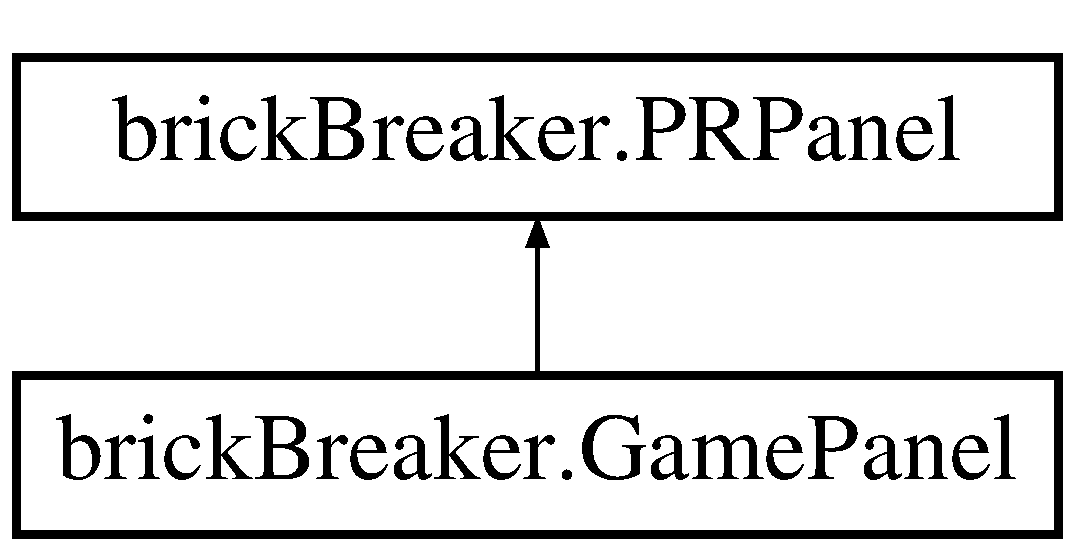
\includegraphics[height=2cm]{classbrick_breaker_1_1_game_panel}
\end{center}
\end{figure}
\subsection*{Public Member Functions}
\begin{DoxyCompactItemize}
\item 
\hyperlink{classbrick_breaker_1_1_game_panel_a9babd944824d2c3462b8dbdc099d65b4}{GamePanel} (\hyperlink{classbrick_breaker_1_1_level}{Level} lev, \hyperlink{classbrick_breaker_1_1_start}{Start} main)
\item 
void \hyperlink{classbrick_breaker_1_1_game_panel_a55dcdeddbe45e2a0d1b4e3ac792aefc4}{reset} (\hyperlink{classbrick_breaker_1_1_level}{Level} lev)
\item 
\hypertarget{classbrick_breaker_1_1_game_panel_a65a1fcc7b053868c7ee654c10036c4a0}{
void {\bfseries init} ()}
\label{classbrick_breaker_1_1_game_panel_a65a1fcc7b053868c7ee654c10036c4a0}

\item 
void \hyperlink{classbrick_breaker_1_1_game_panel_ac06637c2b612d44711aebefde82249bc}{start} ()
\item 
void \hyperlink{classbrick_breaker_1_1_game_panel_adda952b668cd479832134a4c0ddfbc41}{stop} ()
\item 
void \hyperlink{classbrick_breaker_1_1_game_panel_a74382da15296d8ed9be081e4e6af72cc}{pause} ()
\item 
void \hyperlink{classbrick_breaker_1_1_game_panel_af987d9ffe6d1d68941a93547bab41cfe}{resume} ()
\item 
void \hyperlink{classbrick_breaker_1_1_game_panel_a9ede756878b9f1056369baa900dcbc4f}{actionPerformed} (ActionEvent e)
\item 
void \hyperlink{classbrick_breaker_1_1_game_panel_abf3d766d8fff87e69bfaf8ff59c438f3}{keyPressed} (KeyEvent e)
\item 
void \hyperlink{classbrick_breaker_1_1_game_panel_a8c41cc926e88dc8d1a1c241e6b9ef12e}{keyReleased} (KeyEvent e)
\item 
void \hyperlink{classbrick_breaker_1_1_game_panel_a23a455353c5904274a39f0f224cb0005}{keyTyped} (KeyEvent e)
\end{DoxyCompactItemize}
\subsection*{Static Public Attributes}
\begin{DoxyCompactItemize}
\item 
\hypertarget{classbrick_breaker_1_1_game_panel_ade79ff9ff8f4de5cfa2f02fe8701e12d}{
static final int {\bfseries PWIDTH} = 1000}
\label{classbrick_breaker_1_1_game_panel_ade79ff9ff8f4de5cfa2f02fe8701e12d}

\item 
\hypertarget{classbrick_breaker_1_1_game_panel_a91b8f40423595d7b8736d6c0e8e3ce2e}{
static final int {\bfseries PHEIGHT} = 700}
\label{classbrick_breaker_1_1_game_panel_a91b8f40423595d7b8736d6c0e8e3ce2e}

\item 
\hypertarget{classbrick_breaker_1_1_game_panel_ac4460432a58e6284b97eaa6a08e69858}{
static final int {\bfseries BORDER} = 10}
\label{classbrick_breaker_1_1_game_panel_ac4460432a58e6284b97eaa6a08e69858}

\item 
\hypertarget{classbrick_breaker_1_1_game_panel_a59de5a835b862d59d91cf561eae7e87f}{
static final int {\bfseries ARENA\_\-WIDTH} = PWIDTH -\/ 2$\ast$BORDER}
\label{classbrick_breaker_1_1_game_panel_a59de5a835b862d59d91cf561eae7e87f}

\item 
\hypertarget{classbrick_breaker_1_1_game_panel_af1a2ab5d5cf158f0231a00ba886a8a10}{
static final int {\bfseries ARENA\_\-HEIGHT} = PHEIGHT -\/ 2$\ast$BORDER}
\label{classbrick_breaker_1_1_game_panel_af1a2ab5d5cf158f0231a00ba886a8a10}

\end{DoxyCompactItemize}


\subsection{Constructor \& Destructor Documentation}
\hypertarget{classbrick_breaker_1_1_game_panel_a9babd944824d2c3462b8dbdc099d65b4}{
\index{brickBreaker::GamePanel@{brickBreaker::GamePanel}!GamePanel@{GamePanel}}
\index{GamePanel@{GamePanel}!brickBreaker::GamePanel@{brickBreaker::GamePanel}}
\subsubsection[{GamePanel}]{\setlength{\rightskip}{0pt plus 5cm}brickBreaker.GamePanel.GamePanel ({\bf Level} {\em lev}, \/  {\bf Start} {\em main})}}
\label{classbrick_breaker_1_1_game_panel_a9babd944824d2c3462b8dbdc099d65b4}
\hyperlink{classbrick_breaker_1_1_game_panel}{GamePanel} constructor. 
\begin{DoxyParams}{Parameters}
\item[{\em lev}]\hyperlink{classbrick_breaker_1_1_level}{Level} object containing the components to be used in this game \item[{\em main}]The main \hyperlink{classbrick_breaker_1_1_start}{Start} object used to flip panels when the game is over \end{DoxyParams}


\subsection{Member Function Documentation}
\hypertarget{classbrick_breaker_1_1_game_panel_a9ede756878b9f1056369baa900dcbc4f}{
\index{brickBreaker::GamePanel@{brickBreaker::GamePanel}!actionPerformed@{actionPerformed}}
\index{actionPerformed@{actionPerformed}!brickBreaker::GamePanel@{brickBreaker::GamePanel}}
\subsubsection[{actionPerformed}]{\setlength{\rightskip}{0pt plus 5cm}void brickBreaker.GamePanel.actionPerformed (ActionEvent {\em e})}}
\label{classbrick_breaker_1_1_game_panel_a9ede756878b9f1056369baa900dcbc4f}
Repeatedly update, render and sleep. This method is automatically called every time the timer updates. 
\begin{DoxyParams}{Parameters}
\item[{\em e}]ActionEvent generated by the timer. \end{DoxyParams}
\hypertarget{classbrick_breaker_1_1_game_panel_abf3d766d8fff87e69bfaf8ff59c438f3}{
\index{brickBreaker::GamePanel@{brickBreaker::GamePanel}!keyPressed@{keyPressed}}
\index{keyPressed@{keyPressed}!brickBreaker::GamePanel@{brickBreaker::GamePanel}}
\subsubsection[{keyPressed}]{\setlength{\rightskip}{0pt plus 5cm}void brickBreaker.GamePanel.keyPressed (KeyEvent {\em e})}}
\label{classbrick_breaker_1_1_game_panel_abf3d766d8fff87e69bfaf8ff59c438f3}
Processes the key event, either leaving the game or moving a racket. 
\begin{DoxyParams}{Parameters}
\item[{\em e}]Generate KeyEvent corresponding to the key that has been pressed. \end{DoxyParams}


Reimplemented from \hyperlink{classbrick_breaker_1_1_p_r_panel_af86ccc2d42dc48eb03fb6db22e593fc2}{brickBreaker.PRPanel}.

\hypertarget{classbrick_breaker_1_1_game_panel_a8c41cc926e88dc8d1a1c241e6b9ef12e}{
\index{brickBreaker::GamePanel@{brickBreaker::GamePanel}!keyReleased@{keyReleased}}
\index{keyReleased@{keyReleased}!brickBreaker::GamePanel@{brickBreaker::GamePanel}}
\subsubsection[{keyReleased}]{\setlength{\rightskip}{0pt plus 5cm}void brickBreaker.GamePanel.keyReleased (KeyEvent {\em e})}}
\label{classbrick_breaker_1_1_game_panel_a8c41cc926e88dc8d1a1c241e6b9ef12e}
Passes the key event on to the level player, which stops the corresponding racket from moving. 
\begin{DoxyParams}{Parameters}
\item[{\em e}]Generate KeyEvent corresponding to the key that has been pressed. \end{DoxyParams}


Reimplemented from \hyperlink{classbrick_breaker_1_1_p_r_panel_a3485136bec68dd500b98039bd7a87e8e}{brickBreaker.PRPanel}.

\hypertarget{classbrick_breaker_1_1_game_panel_a23a455353c5904274a39f0f224cb0005}{
\index{brickBreaker::GamePanel@{brickBreaker::GamePanel}!keyTyped@{keyTyped}}
\index{keyTyped@{keyTyped}!brickBreaker::GamePanel@{brickBreaker::GamePanel}}
\subsubsection[{keyTyped}]{\setlength{\rightskip}{0pt plus 5cm}void brickBreaker.GamePanel.keyTyped (KeyEvent {\em e})}}
\label{classbrick_breaker_1_1_game_panel_a23a455353c5904274a39f0f224cb0005}
Takes no action. 
\begin{DoxyParams}{Parameters}
\item[{\em e}]Generate KeyEvent corresponding to the key that has been pressed. \end{DoxyParams}


Reimplemented from \hyperlink{classbrick_breaker_1_1_p_r_panel_a51bdf51ab7141c16101753e4180c970a}{brickBreaker.PRPanel}.

\hypertarget{classbrick_breaker_1_1_game_panel_a74382da15296d8ed9be081e4e6af72cc}{
\index{brickBreaker::GamePanel@{brickBreaker::GamePanel}!pause@{pause}}
\index{pause@{pause}!brickBreaker::GamePanel@{brickBreaker::GamePanel}}
\subsubsection[{pause}]{\setlength{\rightskip}{0pt plus 5cm}void brickBreaker.GamePanel.pause ()}}
\label{classbrick_breaker_1_1_game_panel_a74382da15296d8ed9be081e4e6af72cc}
Pauses gameplay. The clock continues running and painting the screen, but game components are not updated. 

Reimplemented from \hyperlink{classbrick_breaker_1_1_p_r_panel_a0868e501fc5599973492e6f0c53da920}{brickBreaker.PRPanel}.

\hypertarget{classbrick_breaker_1_1_game_panel_a55dcdeddbe45e2a0d1b4e3ac792aefc4}{
\index{brickBreaker::GamePanel@{brickBreaker::GamePanel}!reset@{reset}}
\index{reset@{reset}!brickBreaker::GamePanel@{brickBreaker::GamePanel}}
\subsubsection[{reset}]{\setlength{\rightskip}{0pt plus 5cm}void brickBreaker.GamePanel.reset ({\bf Level} {\em lev})}}
\label{classbrick_breaker_1_1_game_panel_a55dcdeddbe45e2a0d1b4e3ac792aefc4}
Resets the game to its initial state. 
\begin{DoxyParams}{Parameters}
\item[{\em lev}]\hyperlink{classbrick_breaker_1_1_level}{Level} object containing all the initial components in this game \end{DoxyParams}
\hypertarget{classbrick_breaker_1_1_game_panel_af987d9ffe6d1d68941a93547bab41cfe}{
\index{brickBreaker::GamePanel@{brickBreaker::GamePanel}!resume@{resume}}
\index{resume@{resume}!brickBreaker::GamePanel@{brickBreaker::GamePanel}}
\subsubsection[{resume}]{\setlength{\rightskip}{0pt plus 5cm}void brickBreaker.GamePanel.resume ()}}
\label{classbrick_breaker_1_1_game_panel_af987d9ffe6d1d68941a93547bab41cfe}
Resumes gameplay 

Reimplemented from \hyperlink{classbrick_breaker_1_1_p_r_panel_ac9aadc88543f9032a27f3eb2b8ea908b}{brickBreaker.PRPanel}.

\hypertarget{classbrick_breaker_1_1_game_panel_ac06637c2b612d44711aebefde82249bc}{
\index{brickBreaker::GamePanel@{brickBreaker::GamePanel}!start@{start}}
\index{start@{start}!brickBreaker::GamePanel@{brickBreaker::GamePanel}}
\subsubsection[{start}]{\setlength{\rightskip}{0pt plus 5cm}void brickBreaker.GamePanel.start ()}}
\label{classbrick_breaker_1_1_game_panel_ac06637c2b612d44711aebefde82249bc}
Resets the ball position and score to zero and starts the clock. 

Reimplemented from \hyperlink{classbrick_breaker_1_1_p_r_panel_a94e190e70d6aa937068cbf5e8cff523e}{brickBreaker.PRPanel}.

\hypertarget{classbrick_breaker_1_1_game_panel_adda952b668cd479832134a4c0ddfbc41}{
\index{brickBreaker::GamePanel@{brickBreaker::GamePanel}!stop@{stop}}
\index{stop@{stop}!brickBreaker::GamePanel@{brickBreaker::GamePanel}}
\subsubsection[{stop}]{\setlength{\rightskip}{0pt plus 5cm}void brickBreaker.GamePanel.stop ()}}
\label{classbrick_breaker_1_1_game_panel_adda952b668cd479832134a4c0ddfbc41}
Stops gameplay 

Reimplemented from \hyperlink{classbrick_breaker_1_1_p_r_panel_ad077fab978f84663f366a6fdde5efe6c}{brickBreaker.PRPanel}.



The documentation for this class was generated from the following file:\begin{DoxyCompactItemize}
\item 
src/game/brickBreaker/\hyperlink{_game_panel_8java}{GamePanel.java}\end{DoxyCompactItemize}

\hypertarget{classbrick_breaker_1_1web_1_1_high_score}{
\section{brickBreaker.web.HighScore Class Reference}
\label{classbrick_breaker_1_1web_1_1_high_score}\index{brickBreaker::web::HighScore@{brickBreaker::web::HighScore}}
}
\subsection*{Public Member Functions}
\begin{DoxyCompactItemize}
\item 
\hyperlink{classbrick_breaker_1_1web_1_1_high_score_abf16c56c51bfefd032d36228ddb8324d}{HighScore} (String name, long score)
\item 
String \hyperlink{classbrick_breaker_1_1web_1_1_high_score_afc959404f76813aeb079bf435bb6a52d}{getName} ()
\item 
long \hyperlink{classbrick_breaker_1_1web_1_1_high_score_a8f8c2b28d7975e261286f5dfb6d62752}{getScore} ()
\end{DoxyCompactItemize}


\subsection{Detailed Description}
This class provides a representation of a high score with a name and score.

\begin{DoxyAuthor}{Author}
Abraham Lin 
\end{DoxyAuthor}


\subsection{Constructor \& Destructor Documentation}
\hypertarget{classbrick_breaker_1_1web_1_1_high_score_abf16c56c51bfefd032d36228ddb8324d}{
\index{brickBreaker::web::HighScore@{brickBreaker::web::HighScore}!HighScore@{HighScore}}
\index{HighScore@{HighScore}!brickBreaker::web::HighScore@{brickBreaker::web::HighScore}}
\subsubsection[{HighScore}]{\setlength{\rightskip}{0pt plus 5cm}brickBreaker.web.HighScore.HighScore (String {\em name}, \/  long {\em score})}}
\label{classbrick_breaker_1_1web_1_1_high_score_abf16c56c51bfefd032d36228ddb8324d}
Constructs a new high score with the specified name and score.


\begin{DoxyParams}{Parameters}
\item[{\em name}]the name \item[{\em score}]the score \end{DoxyParams}


\subsection{Member Function Documentation}
\hypertarget{classbrick_breaker_1_1web_1_1_high_score_afc959404f76813aeb079bf435bb6a52d}{
\index{brickBreaker::web::HighScore@{brickBreaker::web::HighScore}!getName@{getName}}
\index{getName@{getName}!brickBreaker::web::HighScore@{brickBreaker::web::HighScore}}
\subsubsection[{getName}]{\setlength{\rightskip}{0pt plus 5cm}String brickBreaker.web.HighScore.getName ()}}
\label{classbrick_breaker_1_1web_1_1_high_score_afc959404f76813aeb079bf435bb6a52d}
Returns the name associated with this high score.

\begin{DoxyReturn}{Returns}
the associated name 
\end{DoxyReturn}
\hypertarget{classbrick_breaker_1_1web_1_1_high_score_a8f8c2b28d7975e261286f5dfb6d62752}{
\index{brickBreaker::web::HighScore@{brickBreaker::web::HighScore}!getScore@{getScore}}
\index{getScore@{getScore}!brickBreaker::web::HighScore@{brickBreaker::web::HighScore}}
\subsubsection[{getScore}]{\setlength{\rightskip}{0pt plus 5cm}long brickBreaker.web.HighScore.getScore ()}}
\label{classbrick_breaker_1_1web_1_1_high_score_a8f8c2b28d7975e261286f5dfb6d62752}
Returns the score associated with this high score.

\begin{DoxyReturn}{Returns}
the associated score 
\end{DoxyReturn}


The documentation for this class was generated from the following file:\begin{DoxyCompactItemize}
\item 
src/game/brickBreaker/web/HighScore.java\end{DoxyCompactItemize}

\hypertarget{classbrick_breaker_1_1_horizontal_racket}{
\section{brickBreaker.HorizontalRacket Class Reference}
\label{classbrick_breaker_1_1_horizontal_racket}\index{brickBreaker::HorizontalRacket@{brickBreaker::HorizontalRacket}}
}
Inheritance diagram for brickBreaker.HorizontalRacket:\begin{figure}[H]
\begin{center}
\leavevmode
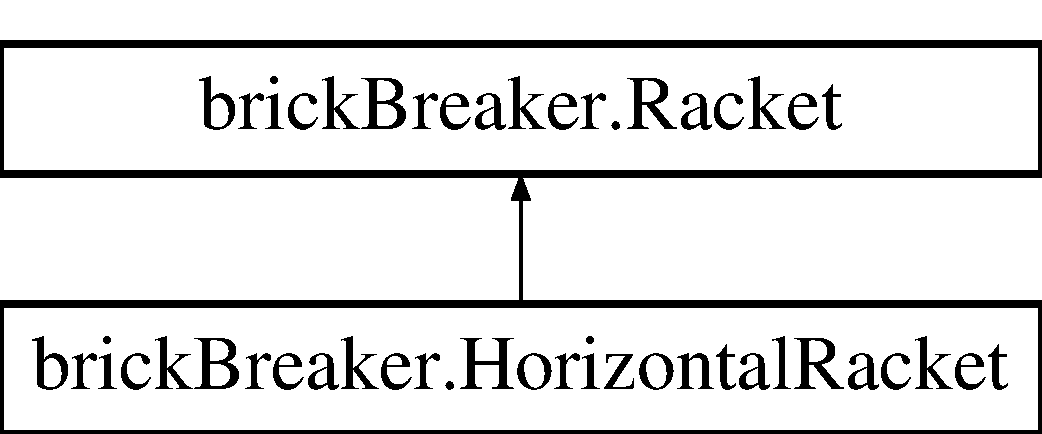
\includegraphics[height=2cm]{classbrick_breaker_1_1_horizontal_racket}
\end{center}
\end{figure}
\subsection*{Public Member Functions}
\begin{DoxyCompactItemize}
\item 
\hyperlink{classbrick_breaker_1_1_horizontal_racket_aecf9f4abdeda94cc4477603aec0d3640}{HorizontalRacket} (int arenaW, int arenaH, int racketW, boolean top)
\item 
void \hyperlink{classbrick_breaker_1_1_horizontal_racket_a8d97c411da71162acd5ecbb32c333f8d}{draw} (Graphics g)
\item 
\hyperlink{classbrick_breaker_1_1_ball}{Ball} \hyperlink{classbrick_breaker_1_1_horizontal_racket_a0a504cfa7af83740b19435e73ecd7975}{checkCollision} (\hyperlink{classbrick_breaker_1_1_ball}{Ball} ball)
\item 
boolean \hyperlink{classbrick_breaker_1_1_horizontal_racket_a183d1d47f35fad74e603534ec74fbdb9}{checkPast} (\hyperlink{classbrick_breaker_1_1_ball}{Ball} ball)
\item 
boolean \hyperlink{classbrick_breaker_1_1_horizontal_racket_a12688619999a3e4d302449ab4bcd0e3d}{isTop} ()
\item 
boolean \hyperlink{classbrick_breaker_1_1_horizontal_racket_aef823257f470172eb2caacfa95a61b99}{isBottom} ()
\end{DoxyCompactItemize}


\subsection{Constructor \& Destructor Documentation}
\hypertarget{classbrick_breaker_1_1_horizontal_racket_aecf9f4abdeda94cc4477603aec0d3640}{
\index{brickBreaker::HorizontalRacket@{brickBreaker::HorizontalRacket}!HorizontalRacket@{HorizontalRacket}}
\index{HorizontalRacket@{HorizontalRacket}!brickBreaker::HorizontalRacket@{brickBreaker::HorizontalRacket}}
\subsubsection[{HorizontalRacket}]{\setlength{\rightskip}{0pt plus 5cm}brickBreaker.HorizontalRacket.HorizontalRacket (int {\em arenaW}, \/  int {\em arenaH}, \/  int {\em racketW}, \/  boolean {\em top})}}
\label{classbrick_breaker_1_1_horizontal_racket_aecf9f4abdeda94cc4477603aec0d3640}
Initializes the \hyperlink{classbrick_breaker_1_1_horizontal_racket}{HorizontalRacket} on the screen.


\begin{DoxyParams}{Parameters}
\item[{\em arenaW}]The width of the screen on which play occurs \item[{\em arenaH}]The height of the screen on which play occurs \item[{\em racketW}]The width of the racket, in pixels \item[{\em top}]True if the racket is at the top of the screen, false if it is at the bottom \end{DoxyParams}


\subsection{Member Function Documentation}
\hypertarget{classbrick_breaker_1_1_horizontal_racket_a0a504cfa7af83740b19435e73ecd7975}{
\index{brickBreaker::HorizontalRacket@{brickBreaker::HorizontalRacket}!checkCollision@{checkCollision}}
\index{checkCollision@{checkCollision}!brickBreaker::HorizontalRacket@{brickBreaker::HorizontalRacket}}
\subsubsection[{checkCollision}]{\setlength{\rightskip}{0pt plus 5cm}{\bf Ball} brickBreaker.HorizontalRacket.checkCollision ({\bf Ball} {\em ball})\hspace{0.3cm}{\ttfamily  \mbox{[}virtual\mbox{]}}}}
\label{classbrick_breaker_1_1_horizontal_racket_a0a504cfa7af83740b19435e73ecd7975}
Checks if the ball collides with the racket and updates the ball's position and direction.


\begin{DoxyParams}{Parameters}
\item[{\em ball}]The ball object to be tested \end{DoxyParams}
\begin{DoxyReturn}{Returns}
Returns the updated ball object 
\end{DoxyReturn}


Implements \hyperlink{classbrick_breaker_1_1_racket_a81880bdbdfda6ec88d1d4e7fc72f8f74}{brickBreaker.Racket}.

\hypertarget{classbrick_breaker_1_1_horizontal_racket_a183d1d47f35fad74e603534ec74fbdb9}{
\index{brickBreaker::HorizontalRacket@{brickBreaker::HorizontalRacket}!checkPast@{checkPast}}
\index{checkPast@{checkPast}!brickBreaker::HorizontalRacket@{brickBreaker::HorizontalRacket}}
\subsubsection[{checkPast}]{\setlength{\rightskip}{0pt plus 5cm}boolean brickBreaker.HorizontalRacket.checkPast ({\bf Ball} {\em ball})\hspace{0.3cm}{\ttfamily  \mbox{[}virtual\mbox{]}}}}
\label{classbrick_breaker_1_1_horizontal_racket_a183d1d47f35fad74e603534ec74fbdb9}
Checks if the ball is past the racket (and thus out of play).


\begin{DoxyParams}{Parameters}
\item[{\em ball}]The ball object to be tested. \end{DoxyParams}
\begin{DoxyReturn}{Returns}
Returns true if the ball has passed the racket, false if it is still in play. 
\end{DoxyReturn}


Implements \hyperlink{classbrick_breaker_1_1_racket_a129dbc802cd26299ebca916283edbe27}{brickBreaker.Racket}.

\hypertarget{classbrick_breaker_1_1_horizontal_racket_a8d97c411da71162acd5ecbb32c333f8d}{
\index{brickBreaker::HorizontalRacket@{brickBreaker::HorizontalRacket}!draw@{draw}}
\index{draw@{draw}!brickBreaker::HorizontalRacket@{brickBreaker::HorizontalRacket}}
\subsubsection[{draw}]{\setlength{\rightskip}{0pt plus 5cm}void brickBreaker.HorizontalRacket.draw (Graphics {\em g})\hspace{0.3cm}{\ttfamily  \mbox{[}virtual\mbox{]}}}}
\label{classbrick_breaker_1_1_horizontal_racket_a8d97c411da71162acd5ecbb32c333f8d}
Draws the racket on the screen.


\begin{DoxyParams}{Parameters}
\item[{\em g}]The graphics object on which to draw \end{DoxyParams}


Implements \hyperlink{classbrick_breaker_1_1_racket_a6ca0308def67e0955522a0e0beb430e9}{brickBreaker.Racket}.

\hypertarget{classbrick_breaker_1_1_horizontal_racket_aef823257f470172eb2caacfa95a61b99}{
\index{brickBreaker::HorizontalRacket@{brickBreaker::HorizontalRacket}!isBottom@{isBottom}}
\index{isBottom@{isBottom}!brickBreaker::HorizontalRacket@{brickBreaker::HorizontalRacket}}
\subsubsection[{isBottom}]{\setlength{\rightskip}{0pt plus 5cm}boolean brickBreaker.HorizontalRacket.isBottom ()}}
\label{classbrick_breaker_1_1_horizontal_racket_aef823257f470172eb2caacfa95a61b99}
\begin{DoxyReturn}{Returns}
Returns true if the racket is at the bottom of the screen. 
\end{DoxyReturn}


Reimplemented from \hyperlink{classbrick_breaker_1_1_racket_a908f0a42e73739db9fd0734d6a4fdb2f}{brickBreaker.Racket}.

\hypertarget{classbrick_breaker_1_1_horizontal_racket_a12688619999a3e4d302449ab4bcd0e3d}{
\index{brickBreaker::HorizontalRacket@{brickBreaker::HorizontalRacket}!isTop@{isTop}}
\index{isTop@{isTop}!brickBreaker::HorizontalRacket@{brickBreaker::HorizontalRacket}}
\subsubsection[{isTop}]{\setlength{\rightskip}{0pt plus 5cm}boolean brickBreaker.HorizontalRacket.isTop ()}}
\label{classbrick_breaker_1_1_horizontal_racket_a12688619999a3e4d302449ab4bcd0e3d}
\begin{DoxyReturn}{Returns}
Returns true if the racket is at the top of the screen. 
\end{DoxyReturn}


Reimplemented from \hyperlink{classbrick_breaker_1_1_racket_a0bd80cbd11ffe9afd6212e2d96a88554}{brickBreaker.Racket}.



The documentation for this class was generated from the following file:\begin{DoxyCompactItemize}
\item 
src/game/brickBreaker/\hyperlink{_horizontal_racket_8java}{HorizontalRacket.java}\end{DoxyCompactItemize}

\hypertarget{classbrick_breaker_1_1_idle_panel}{
\section{brickBreaker.IdlePanel Class Reference}
\label{classbrick_breaker_1_1_idle_panel}\index{brickBreaker::IdlePanel@{brickBreaker::IdlePanel}}
}
Inheritance diagram for brickBreaker.IdlePanel:\begin{figure}[H]
\begin{center}
\leavevmode
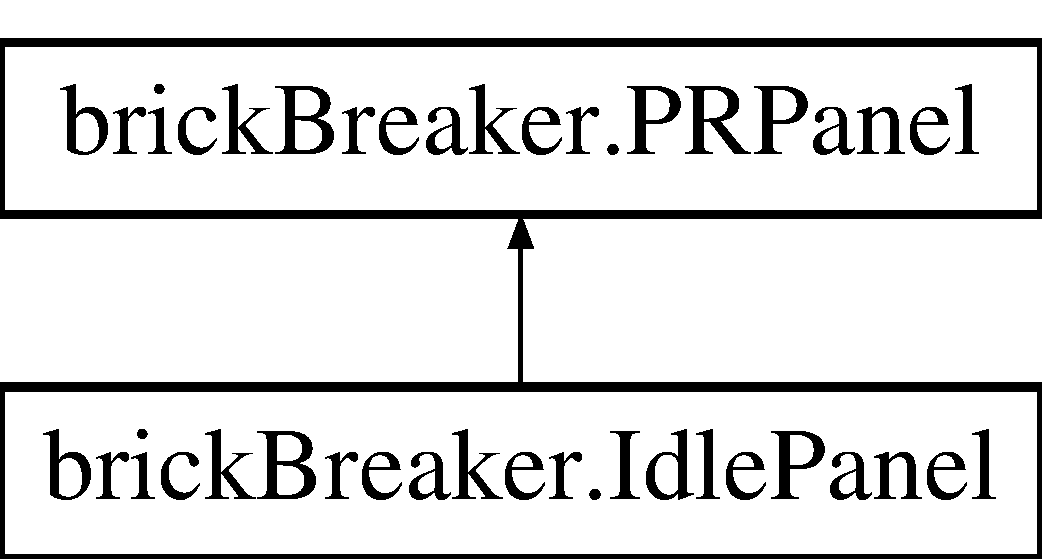
\includegraphics[height=2cm]{classbrick_breaker_1_1_idle_panel}
\end{center}
\end{figure}
\subsection*{Public Member Functions}
\begin{DoxyCompactItemize}
\item 
\hyperlink{classbrick_breaker_1_1_idle_panel_ab4ba4ca56923da71a415ca965a07b0dd}{IdlePanel} (\hyperlink{classbrick_breaker_1_1_start}{Start} s)
\item 
void \hyperlink{classbrick_breaker_1_1_idle_panel_ad391091a78283ca2546e52f967d46ed6}{start} ()
\item 
void \hyperlink{classbrick_breaker_1_1_idle_panel_a42b96627662408932245a672b5fbfaf1}{pause} ()
\item 
void \hyperlink{classbrick_breaker_1_1_idle_panel_ab04b565d2e626077051cefb27772a98f}{resume} ()
\item 
void \hyperlink{classbrick_breaker_1_1_idle_panel_a2334ae977477929eeb82dbba53384360}{stop} ()
\item 
void \hyperlink{classbrick_breaker_1_1_idle_panel_a6d0829251befbc226224838015e9e46d}{reset} ()
\end{DoxyCompactItemize}
\subsection*{Static Public Attributes}
\begin{DoxyCompactItemize}
\item 
\hypertarget{classbrick_breaker_1_1_idle_panel_a58f042f33a11a790b7e7faee8482735f}{
static final int {\bfseries PWIDTH} = 1000}
\label{classbrick_breaker_1_1_idle_panel_a58f042f33a11a790b7e7faee8482735f}

\item 
\hypertarget{classbrick_breaker_1_1_idle_panel_a7ef3a9bc791cbdf50cbb54f10cb80608}{
static final int {\bfseries PHEIGHT} = 700}
\label{classbrick_breaker_1_1_idle_panel_a7ef3a9bc791cbdf50cbb54f10cb80608}

\end{DoxyCompactItemize}


\subsection{Constructor \& Destructor Documentation}
\hypertarget{classbrick_breaker_1_1_idle_panel_ab4ba4ca56923da71a415ca965a07b0dd}{
\index{brickBreaker::IdlePanel@{brickBreaker::IdlePanel}!IdlePanel@{IdlePanel}}
\index{IdlePanel@{IdlePanel}!brickBreaker::IdlePanel@{brickBreaker::IdlePanel}}
\subsubsection[{IdlePanel}]{\setlength{\rightskip}{0pt plus 5cm}brickBreaker.IdlePanel.IdlePanel ({\bf Start} {\em s})}}
\label{classbrick_breaker_1_1_idle_panel_ab4ba4ca56923da71a415ca965a07b0dd}
Constructor.


\begin{DoxyParams}{Parameters}
\item[{\em s}]JFrame which \hyperlink{classbrick_breaker_1_1_idle_panel}{IdlePanel} is a part of \end{DoxyParams}


WebConfig.getInstance().setHost(\char`\"{}brickbreaker.zxq.net\char`\"{}); UserConfig.getInstance().setUsername(\char`\"{}robert\char`\"{}); UserConfig.getInstance().setPassword(\char`\"{}123\char`\"{});



\subsection{Member Function Documentation}
\hypertarget{classbrick_breaker_1_1_idle_panel_a42b96627662408932245a672b5fbfaf1}{
\index{brickBreaker::IdlePanel@{brickBreaker::IdlePanel}!pause@{pause}}
\index{pause@{pause}!brickBreaker::IdlePanel@{brickBreaker::IdlePanel}}
\subsubsection[{pause}]{\setlength{\rightskip}{0pt plus 5cm}void brickBreaker.IdlePanel.pause ()}}
\label{classbrick_breaker_1_1_idle_panel_a42b96627662408932245a672b5fbfaf1}
Pauses \hyperlink{classbrick_breaker_1_1_idle_panel}{IdlePanel} 

Reimplemented from \hyperlink{classbrick_breaker_1_1_p_r_panel}{brickBreaker.PRPanel}.

\hypertarget{classbrick_breaker_1_1_idle_panel_a6d0829251befbc226224838015e9e46d}{
\index{brickBreaker::IdlePanel@{brickBreaker::IdlePanel}!reset@{reset}}
\index{reset@{reset}!brickBreaker::IdlePanel@{brickBreaker::IdlePanel}}
\subsubsection[{reset}]{\setlength{\rightskip}{0pt plus 5cm}void brickBreaker.IdlePanel.reset ()}}
\label{classbrick_breaker_1_1_idle_panel_a6d0829251befbc226224838015e9e46d}
Clears any displayed level and resets the list of levels \hypertarget{classbrick_breaker_1_1_idle_panel_ab04b565d2e626077051cefb27772a98f}{
\index{brickBreaker::IdlePanel@{brickBreaker::IdlePanel}!resume@{resume}}
\index{resume@{resume}!brickBreaker::IdlePanel@{brickBreaker::IdlePanel}}
\subsubsection[{resume}]{\setlength{\rightskip}{0pt plus 5cm}void brickBreaker.IdlePanel.resume ()}}
\label{classbrick_breaker_1_1_idle_panel_ab04b565d2e626077051cefb27772a98f}
Resumes \hyperlink{classbrick_breaker_1_1_idle_panel}{IdlePanel} 

Reimplemented from \hyperlink{classbrick_breaker_1_1_p_r_panel}{brickBreaker.PRPanel}.

\hypertarget{classbrick_breaker_1_1_idle_panel_ad391091a78283ca2546e52f967d46ed6}{
\index{brickBreaker::IdlePanel@{brickBreaker::IdlePanel}!start@{start}}
\index{start@{start}!brickBreaker::IdlePanel@{brickBreaker::IdlePanel}}
\subsubsection[{start}]{\setlength{\rightskip}{0pt plus 5cm}void brickBreaker.IdlePanel.start ()}}
\label{classbrick_breaker_1_1_idle_panel_ad391091a78283ca2546e52f967d46ed6}
Starts \hyperlink{classbrick_breaker_1_1_idle_panel}{IdlePanel} 

Reimplemented from \hyperlink{classbrick_breaker_1_1_p_r_panel}{brickBreaker.PRPanel}.

\hypertarget{classbrick_breaker_1_1_idle_panel_a2334ae977477929eeb82dbba53384360}{
\index{brickBreaker::IdlePanel@{brickBreaker::IdlePanel}!stop@{stop}}
\index{stop@{stop}!brickBreaker::IdlePanel@{brickBreaker::IdlePanel}}
\subsubsection[{stop}]{\setlength{\rightskip}{0pt plus 5cm}void brickBreaker.IdlePanel.stop ()}}
\label{classbrick_breaker_1_1_idle_panel_a2334ae977477929eeb82dbba53384360}
Stops \hyperlink{classbrick_breaker_1_1_idle_panel}{IdlePanel} 

Reimplemented from \hyperlink{classbrick_breaker_1_1_p_r_panel}{brickBreaker.PRPanel}.



The documentation for this class was generated from the following file:\begin{DoxyCompactItemize}
\item 
game/brickBreaker/\hyperlink{_idle_panel_8java}{IdlePanel.java}\end{DoxyCompactItemize}

\hypertarget{classbrick_breaker_1_1web_1_1_invalid_user_exception}{
\section{brickBreaker.web.InvalidUserException Class Reference}
\label{classbrick_breaker_1_1web_1_1_invalid_user_exception}\index{brickBreaker::web::InvalidUserException@{brickBreaker::web::InvalidUserException}}
}
\subsection*{Public Member Functions}
\begin{DoxyCompactItemize}
\item 
\hyperlink{classbrick_breaker_1_1web_1_1_invalid_user_exception_a500ab07a78ed1ea1f51c685772ec3b11}{InvalidUserException} ()
\item 
\hyperlink{classbrick_breaker_1_1web_1_1_invalid_user_exception_a28a46f03e800b69aca69071687c4a53d}{InvalidUserException} (String message)
\item 
\hyperlink{classbrick_breaker_1_1web_1_1_invalid_user_exception_a1b99af54f90e802a18f6eb4b65cfa5aa}{InvalidUserException} (String message, Throwable cause)
\item 
\hyperlink{classbrick_breaker_1_1web_1_1_invalid_user_exception_a3d20137414f9e52364048c36045ffac0}{InvalidUserException} (Throwable cause)
\end{DoxyCompactItemize}


\subsection{Detailed Description}
This class provides an application-\/specific wrapper for exceptions caused by a failure to authenticate against a remote server.

\begin{DoxyAuthor}{Author}
Abraham Lin 
\end{DoxyAuthor}


\subsection{Constructor \& Destructor Documentation}
\hypertarget{classbrick_breaker_1_1web_1_1_invalid_user_exception_a500ab07a78ed1ea1f51c685772ec3b11}{
\index{brickBreaker::web::InvalidUserException@{brickBreaker::web::InvalidUserException}!InvalidUserException@{InvalidUserException}}
\index{InvalidUserException@{InvalidUserException}!brickBreaker::web::InvalidUserException@{brickBreaker::web::InvalidUserException}}
\subsubsection[{InvalidUserException}]{\setlength{\rightskip}{0pt plus 5cm}brickBreaker.web.InvalidUserException.InvalidUserException ()}}
\label{classbrick_breaker_1_1web_1_1_invalid_user_exception_a500ab07a78ed1ea1f51c685772ec3b11}
Constructs a new {\ttfamily \hyperlink{classbrick_breaker_1_1web_1_1_invalid_user_exception}{InvalidUserException}} with {\ttfamily null} as its detail message. \hypertarget{classbrick_breaker_1_1web_1_1_invalid_user_exception_a28a46f03e800b69aca69071687c4a53d}{
\index{brickBreaker::web::InvalidUserException@{brickBreaker::web::InvalidUserException}!InvalidUserException@{InvalidUserException}}
\index{InvalidUserException@{InvalidUserException}!brickBreaker::web::InvalidUserException@{brickBreaker::web::InvalidUserException}}
\subsubsection[{InvalidUserException}]{\setlength{\rightskip}{0pt plus 5cm}brickBreaker.web.InvalidUserException.InvalidUserException (String {\em message})}}
\label{classbrick_breaker_1_1web_1_1_invalid_user_exception_a28a46f03e800b69aca69071687c4a53d}
Constructs a new {\ttfamily \hyperlink{classbrick_breaker_1_1web_1_1_invalid_user_exception}{InvalidUserException}} with the specified detail message.


\begin{DoxyParams}{Parameters}
\item[{\em message}]the detail message \end{DoxyParams}
\hypertarget{classbrick_breaker_1_1web_1_1_invalid_user_exception_a1b99af54f90e802a18f6eb4b65cfa5aa}{
\index{brickBreaker::web::InvalidUserException@{brickBreaker::web::InvalidUserException}!InvalidUserException@{InvalidUserException}}
\index{InvalidUserException@{InvalidUserException}!brickBreaker::web::InvalidUserException@{brickBreaker::web::InvalidUserException}}
\subsubsection[{InvalidUserException}]{\setlength{\rightskip}{0pt plus 5cm}brickBreaker.web.InvalidUserException.InvalidUserException (String {\em message}, \/  Throwable {\em cause})}}
\label{classbrick_breaker_1_1web_1_1_invalid_user_exception_a1b99af54f90e802a18f6eb4b65cfa5aa}
Constructs a new {\ttfamily \hyperlink{classbrick_breaker_1_1web_1_1_invalid_user_exception}{InvalidUserException}} with the specified detail message and cause.


\begin{DoxyParams}{Parameters}
\item[{\em message}]the detail message \item[{\em cause}]the cause \end{DoxyParams}
\hypertarget{classbrick_breaker_1_1web_1_1_invalid_user_exception_a3d20137414f9e52364048c36045ffac0}{
\index{brickBreaker::web::InvalidUserException@{brickBreaker::web::InvalidUserException}!InvalidUserException@{InvalidUserException}}
\index{InvalidUserException@{InvalidUserException}!brickBreaker::web::InvalidUserException@{brickBreaker::web::InvalidUserException}}
\subsubsection[{InvalidUserException}]{\setlength{\rightskip}{0pt plus 5cm}brickBreaker.web.InvalidUserException.InvalidUserException (Throwable {\em cause})}}
\label{classbrick_breaker_1_1web_1_1_invalid_user_exception_a3d20137414f9e52364048c36045ffac0}
Constructs a new {\ttfamily \hyperlink{classbrick_breaker_1_1web_1_1_invalid_user_exception}{InvalidUserException}} with the specified cause.


\begin{DoxyParams}{Parameters}
\item[{\em cause}]the cause \end{DoxyParams}


The documentation for this class was generated from the following file:\begin{DoxyCompactItemize}
\item 
src/game/brickBreaker/web/InvalidUserException.java\end{DoxyCompactItemize}

\hypertarget{classbrick_breaker_1_1_level}{
\section{brickBreaker.Level Class Reference}
\label{classbrick_breaker_1_1_level}\index{brickBreaker::Level@{brickBreaker::Level}}
}


Inherits java::io::Serializable.

\subsection*{Public Member Functions}
\begin{DoxyCompactItemize}
\item 
\hyperlink{classbrick_breaker_1_1_level_ac98f98fe72c9000911b79fabd548e44e}{Level} (\hyperlink{classbrick_breaker_1_1_brick}{Brick}\mbox{[}$\,$\mbox{]}\mbox{[}$\,$\mbox{]} bricks, \hyperlink{classbrick_breaker_1_1_ball}{Ball}\mbox{[}$\,$\mbox{]} balls, \hyperlink{classbrick_breaker_1_1_racket}{Racket}\mbox{[}$\,$\mbox{]} rack, String name)
\item 
\hyperlink{classbrick_breaker_1_1_level_aa88640ad04ca2a8b471be22a39bd2f75}{Level} (\hyperlink{classbrick_breaker_1_1_brick}{Brick}\mbox{[}$\,$\mbox{]}\mbox{[}$\,$\mbox{]} bricks, \hyperlink{classbrick_breaker_1_1_ball}{Ball}\mbox{[}$\,$\mbox{]} balls, \hyperlink{classbrick_breaker_1_1_racket}{Racket}\mbox{[}$\,$\mbox{]} rack)
\item 
\hyperlink{classbrick_breaker_1_1_level_ab814f5c562c5703aedf3569501b44845}{Level} (\hyperlink{classbrick_breaker_1_1_brick}{Brick}\mbox{[}$\,$\mbox{]}\mbox{[}$\,$\mbox{]} bricks, int players, String name)
\item 
void \hyperlink{classbrick_breaker_1_1_level_a2cf993a57ad58665d34d09b9366a39b4}{initBricks} (\hyperlink{classbrick_breaker_1_1_brick}{Brick}\mbox{[}$\,$\mbox{]}\mbox{[}$\,$\mbox{]} bricks)
\item 
void \hyperlink{classbrick_breaker_1_1_level_a9658a9bfa4707f92de4891f913377202}{setName} (String name)
\item 
\hypertarget{classbrick_breaker_1_1_level_a236ad90c2a8f2193dd154e5b3b424371}{
void {\bfseries setBricks} (\hyperlink{classbrick_breaker_1_1_brick}{Brick}\mbox{[}$\,$\mbox{]}\mbox{[}$\,$\mbox{]} b)}
\label{classbrick_breaker_1_1_level_a236ad90c2a8f2193dd154e5b3b424371}

\item 
\hypertarget{classbrick_breaker_1_1_level_ac52e444e4bbbee478dbf4450932eda60}{
void {\bfseries setRacket} (\hyperlink{classbrick_breaker_1_1_racket}{Racket}\mbox{[}$\,$\mbox{]} r)}
\label{classbrick_breaker_1_1_level_ac52e444e4bbbee478dbf4450932eda60}

\item 
\hypertarget{classbrick_breaker_1_1_level_af4d0305aa2202b4aa4d91a6b37fa262b}{
void {\bfseries setBalls} (\hyperlink{classbrick_breaker_1_1_ball}{Ball}\mbox{[}$\,$\mbox{]} b)}
\label{classbrick_breaker_1_1_level_af4d0305aa2202b4aa4d91a6b37fa262b}

\item 
\hyperlink{classbrick_breaker_1_1_racket}{Racket}\mbox{[}$\,$\mbox{]} \hyperlink{classbrick_breaker_1_1_level_abc80d5b2ae6aa9f6884dddef4a08d82b}{getRackets} ()
\item 
\hyperlink{classbrick_breaker_1_1_ball}{Ball}\mbox{[}$\,$\mbox{]} \hyperlink{classbrick_breaker_1_1_level_aabd74f57cf3043d6bae8b98953344e4b}{getBalls} ()
\item 
\hyperlink{classbrick_breaker_1_1_brick}{Brick}\mbox{[}$\,$\mbox{]}\mbox{[}$\,$\mbox{]} \hyperlink{classbrick_breaker_1_1_level_a32fa1d0bdac9b8fc1b0256b793ebeb8c}{getBricks} ()
\item 
int \hyperlink{classbrick_breaker_1_1_level_a21baab3427644fa78d1b7e98757b3609}{brickWidth} ()
\item 
int \hyperlink{classbrick_breaker_1_1_level_adf924d8f95efb086b49b5709c6b5e48e}{brickHeight} ()
\item 
int \hyperlink{classbrick_breaker_1_1_level_a3bba82793ace6907c19b5b7d21c9d0c2}{numCols} ()
\item 
int \hyperlink{classbrick_breaker_1_1_level_a87616f7c125b41d686d6c50477601200}{numRows} ()
\item 
String \hyperlink{classbrick_breaker_1_1_level_a3ef4e701ca616ff080c401586e04387b}{getName} ()
\end{DoxyCompactItemize}
\subsection*{Static Public Attributes}
\begin{DoxyCompactItemize}
\item 
\hypertarget{classbrick_breaker_1_1_level_ac206c1e0a98a683035f3e199dc993e58}{
static int {\bfseries WIDTH} = GamePanel.ARENA\_\-WIDTH}
\label{classbrick_breaker_1_1_level_ac206c1e0a98a683035f3e199dc993e58}

\item 
\hypertarget{classbrick_breaker_1_1_level_a9e137692bbe309075c83d9d8eef09655}{
static int {\bfseries HEIGHT} = GamePanel.ARENA\_\-HEIGHT}
\label{classbrick_breaker_1_1_level_a9e137692bbe309075c83d9d8eef09655}

\end{DoxyCompactItemize}


\subsection{Constructor \& Destructor Documentation}
\hypertarget{classbrick_breaker_1_1_level_ac98f98fe72c9000911b79fabd548e44e}{
\index{brickBreaker::Level@{brickBreaker::Level}!Level@{Level}}
\index{Level@{Level}!brickBreaker::Level@{brickBreaker::Level}}
\subsubsection[{Level}]{\setlength{\rightskip}{0pt plus 5cm}brickBreaker.Level.Level (Brickbricks\mbox{[}$\,$\mbox{]}\mbox{[}$\,$\mbox{]}, \/  {\bf Ball}\mbox{[}$\,$\mbox{]} {\em balls}, \/  {\bf Racket}\mbox{[}$\,$\mbox{]} {\em rack}, \/  String {\em name})}}
\label{classbrick_breaker_1_1_level_ac98f98fe72c9000911b79fabd548e44e}
Constructor


\begin{DoxyParams}{Parameters}
\item[{\em bricks}]2-\/dimensional array of bricks \item[{\em balls}]All existing balls \item[{\em rack}]All existing rackets \item[{\em name}]String identifier (used in user interface) \end{DoxyParams}
\hypertarget{classbrick_breaker_1_1_level_aa88640ad04ca2a8b471be22a39bd2f75}{
\index{brickBreaker::Level@{brickBreaker::Level}!Level@{Level}}
\index{Level@{Level}!brickBreaker::Level@{brickBreaker::Level}}
\subsubsection[{Level}]{\setlength{\rightskip}{0pt plus 5cm}brickBreaker.Level.Level (Brickbricks\mbox{[}$\,$\mbox{]}\mbox{[}$\,$\mbox{]}, \/  {\bf Ball}\mbox{[}$\,$\mbox{]} {\em balls}, \/  {\bf Racket}\mbox{[}$\,$\mbox{]} {\em rack})}}
\label{classbrick_breaker_1_1_level_aa88640ad04ca2a8b471be22a39bd2f75}
Constructor


\begin{DoxyParams}{Parameters}
\item[{\em bricks}]2-\/dimensional array of bricks \item[{\em balls}]All existing balls \item[{\em rack}]All existing rackets \end{DoxyParams}
\hypertarget{classbrick_breaker_1_1_level_ab814f5c562c5703aedf3569501b44845}{
\index{brickBreaker::Level@{brickBreaker::Level}!Level@{Level}}
\index{Level@{Level}!brickBreaker::Level@{brickBreaker::Level}}
\subsubsection[{Level}]{\setlength{\rightskip}{0pt plus 5cm}brickBreaker.Level.Level ({\bf Brick} {\em bricks}\mbox{[}$\,$\mbox{]}\mbox{[}$\,$\mbox{]}, \/  int {\em players}, \/  String {\em name})}}
\label{classbrick_breaker_1_1_level_ab814f5c562c5703aedf3569501b44845}
Constructor


\begin{DoxyParams}{Parameters}
\item[{\em bricks}]2-\/dimensional array of bricks \item[{\em players}]Number of players \item[{\em name}]String identifier (used in user interface) \end{DoxyParams}


\subsection{Member Function Documentation}
\hypertarget{classbrick_breaker_1_1_level_adf924d8f95efb086b49b5709c6b5e48e}{
\index{brickBreaker::Level@{brickBreaker::Level}!brickHeight@{brickHeight}}
\index{brickHeight@{brickHeight}!brickBreaker::Level@{brickBreaker::Level}}
\subsubsection[{brickHeight}]{\setlength{\rightskip}{0pt plus 5cm}int brickBreaker.Level.brickHeight ()}}
\label{classbrick_breaker_1_1_level_adf924d8f95efb086b49b5709c6b5e48e}
\begin{DoxyReturn}{Returns}
The height of each brick (in pixels) 
\end{DoxyReturn}
\hypertarget{classbrick_breaker_1_1_level_a21baab3427644fa78d1b7e98757b3609}{
\index{brickBreaker::Level@{brickBreaker::Level}!brickWidth@{brickWidth}}
\index{brickWidth@{brickWidth}!brickBreaker::Level@{brickBreaker::Level}}
\subsubsection[{brickWidth}]{\setlength{\rightskip}{0pt plus 5cm}int brickBreaker.Level.brickWidth ()}}
\label{classbrick_breaker_1_1_level_a21baab3427644fa78d1b7e98757b3609}
\begin{DoxyReturn}{Returns}
The width of each brick (in pixels) 
\end{DoxyReturn}
\hypertarget{classbrick_breaker_1_1_level_aabd74f57cf3043d6bae8b98953344e4b}{
\index{brickBreaker::Level@{brickBreaker::Level}!getBalls@{getBalls}}
\index{getBalls@{getBalls}!brickBreaker::Level@{brickBreaker::Level}}
\subsubsection[{getBalls}]{\setlength{\rightskip}{0pt plus 5cm}{\bf Ball} \mbox{[}$\,$\mbox{]} brickBreaker.Level.getBalls ()}}
\label{classbrick_breaker_1_1_level_aabd74f57cf3043d6bae8b98953344e4b}
\begin{DoxyReturn}{Returns}
The array of balls 
\end{DoxyReturn}
\hypertarget{classbrick_breaker_1_1_level_a32fa1d0bdac9b8fc1b0256b793ebeb8c}{
\index{brickBreaker::Level@{brickBreaker::Level}!getBricks@{getBricks}}
\index{getBricks@{getBricks}!brickBreaker::Level@{brickBreaker::Level}}
\subsubsection[{getBricks}]{\setlength{\rightskip}{0pt plus 5cm}{\bf Brick} \mbox{[}$\,$\mbox{]}\mbox{[}$\,$\mbox{]} brickBreaker.Level.getBricks ()}}
\label{classbrick_breaker_1_1_level_a32fa1d0bdac9b8fc1b0256b793ebeb8c}
\begin{DoxyReturn}{Returns}
The 2d array of bricks 
\end{DoxyReturn}
\hypertarget{classbrick_breaker_1_1_level_a3ef4e701ca616ff080c401586e04387b}{
\index{brickBreaker::Level@{brickBreaker::Level}!getName@{getName}}
\index{getName@{getName}!brickBreaker::Level@{brickBreaker::Level}}
\subsubsection[{getName}]{\setlength{\rightskip}{0pt plus 5cm}String brickBreaker.Level.getName ()}}
\label{classbrick_breaker_1_1_level_a3ef4e701ca616ff080c401586e04387b}
\begin{DoxyReturn}{Returns}
The name of this level 
\end{DoxyReturn}
\hypertarget{classbrick_breaker_1_1_level_abc80d5b2ae6aa9f6884dddef4a08d82b}{
\index{brickBreaker::Level@{brickBreaker::Level}!getRackets@{getRackets}}
\index{getRackets@{getRackets}!brickBreaker::Level@{brickBreaker::Level}}
\subsubsection[{getRackets}]{\setlength{\rightskip}{0pt plus 5cm}{\bf Racket} \mbox{[}$\,$\mbox{]} brickBreaker.Level.getRackets ()}}
\label{classbrick_breaker_1_1_level_abc80d5b2ae6aa9f6884dddef4a08d82b}
\begin{DoxyReturn}{Returns}
The array of rackets 
\end{DoxyReturn}
\hypertarget{classbrick_breaker_1_1_level_a2cf993a57ad58665d34d09b9366a39b4}{
\index{brickBreaker::Level@{brickBreaker::Level}!initBricks@{initBricks}}
\index{initBricks@{initBricks}!brickBreaker::Level@{brickBreaker::Level}}
\subsubsection[{initBricks}]{\setlength{\rightskip}{0pt plus 5cm}void brickBreaker.Level.initBricks ({\bf Brick} {\em bricks}\mbox{[}$\,$\mbox{]}\mbox{[}$\,$\mbox{]})}}
\label{classbrick_breaker_1_1_level_a2cf993a57ad58665d34d09b9366a39b4}
Sets the location of each brick in the level. 
\begin{DoxyParams}{Parameters}
\item[{\em bricks}]2d array of all existing bricks \end{DoxyParams}
\hypertarget{classbrick_breaker_1_1_level_a3bba82793ace6907c19b5b7d21c9d0c2}{
\index{brickBreaker::Level@{brickBreaker::Level}!numCols@{numCols}}
\index{numCols@{numCols}!brickBreaker::Level@{brickBreaker::Level}}
\subsubsection[{numCols}]{\setlength{\rightskip}{0pt plus 5cm}int brickBreaker.Level.numCols ()}}
\label{classbrick_breaker_1_1_level_a3bba82793ace6907c19b5b7d21c9d0c2}
\begin{DoxyReturn}{Returns}
The number of columns of bricks across the screen 
\end{DoxyReturn}
\hypertarget{classbrick_breaker_1_1_level_a87616f7c125b41d686d6c50477601200}{
\index{brickBreaker::Level@{brickBreaker::Level}!numRows@{numRows}}
\index{numRows@{numRows}!brickBreaker::Level@{brickBreaker::Level}}
\subsubsection[{numRows}]{\setlength{\rightskip}{0pt plus 5cm}int brickBreaker.Level.numRows ()}}
\label{classbrick_breaker_1_1_level_a87616f7c125b41d686d6c50477601200}
\begin{DoxyReturn}{Returns}
The number of rows of bricks down the screen 
\end{DoxyReturn}
\hypertarget{classbrick_breaker_1_1_level_a9658a9bfa4707f92de4891f913377202}{
\index{brickBreaker::Level@{brickBreaker::Level}!setName@{setName}}
\index{setName@{setName}!brickBreaker::Level@{brickBreaker::Level}}
\subsubsection[{setName}]{\setlength{\rightskip}{0pt plus 5cm}void brickBreaker.Level.setName (String {\em name})}}
\label{classbrick_breaker_1_1_level_a9658a9bfa4707f92de4891f913377202}
Sets the level's name to the new string 
\begin{DoxyParams}{Parameters}
\item[{\em name}]New name \end{DoxyParams}


The documentation for this class was generated from the following file:\begin{DoxyCompactItemize}
\item 
game/brickBreaker/\hyperlink{_level_8java}{Level.java}\end{DoxyCompactItemize}

\hypertarget{classbrick_breaker_1_1local_1_1_level_catalog}{
\section{brickBreaker.local.LevelCatalog Class Reference}
\label{classbrick_breaker_1_1local_1_1_level_catalog}\index{brickBreaker::local::LevelCatalog@{brickBreaker::local::LevelCatalog}}
}
\subsection*{Public Member Functions}
\begin{DoxyCompactItemize}
\item 
void \hyperlink{classbrick_breaker_1_1local_1_1_level_catalog_a3cb48b330d53535457d9aeb4f2f7fb32}{reset} ()  throws FilesystemFailureException 
\item 
List$<$ \hyperlink{classbrick_breaker_1_1_level}{Level} $>$ \hyperlink{classbrick_breaker_1_1local_1_1_level_catalog_a34873e8d58b5e3570da7312b714f1e13}{getLevels} ()
\item 
void \hyperlink{classbrick_breaker_1_1local_1_1_level_catalog_a81201df02f319ba10645c3ee711cb777}{addLevel} (\hyperlink{classbrick_breaker_1_1_level}{Level} level)  throws FilesystemFailureException 
\item 
String \hyperlink{classbrick_breaker_1_1local_1_1_level_catalog_acb192b0db7f4a495d3674fa6b6996a56}{getLevelID} (\hyperlink{classbrick_breaker_1_1_level}{Level} level)
\end{DoxyCompactItemize}
\subsection*{Static Public Member Functions}
\begin{DoxyCompactItemize}
\item 
static \hyperlink{classbrick_breaker_1_1local_1_1_level_catalog}{LevelCatalog} \hyperlink{classbrick_breaker_1_1local_1_1_level_catalog_abeb4b9d17e6743896f3f02eeaa571a42}{getInstance} ()
\end{DoxyCompactItemize}
\subsection*{Static Package Functions}
\begin{DoxyCompactItemize}
\item 
\hypertarget{classbrick_breaker_1_1local_1_1_level_catalog_a7163b269c7bce462b7cf90bbd992a500}{
{\bfseries \mbox{[}static initializer\mbox{]}}}
\label{classbrick_breaker_1_1local_1_1_level_catalog_a7163b269c7bce462b7cf90bbd992a500}

\end{DoxyCompactItemize}


\subsection{Detailed Description}
This singleton class provides an in-\/memory catalog of levels available for use by the application.

\begin{DoxyAuthor}{Author}
Abraham Lin 
\end{DoxyAuthor}


\subsection{Member Function Documentation}
\hypertarget{classbrick_breaker_1_1local_1_1_level_catalog_a81201df02f319ba10645c3ee711cb777}{
\index{brickBreaker::local::LevelCatalog@{brickBreaker::local::LevelCatalog}!addLevel@{addLevel}}
\index{addLevel@{addLevel}!brickBreaker::local::LevelCatalog@{brickBreaker::local::LevelCatalog}}
\subsubsection[{addLevel}]{\setlength{\rightskip}{0pt plus 5cm}void brickBreaker.local.LevelCatalog.addLevel ({\bf Level} {\em level})  throws {\bf FilesystemFailureException} }}
\label{classbrick_breaker_1_1local_1_1_level_catalog_a81201df02f319ba10645c3ee711cb777}
Adds a new level to the catalog, saving it to disk if necessary.


\begin{DoxyParams}{Parameters}
\item[{\em level}]the level to add\end{DoxyParams}

\begin{DoxyExceptions}{Exceptions}
\item[{\em \hyperlink{classbrick_breaker_1_1local_1_1_filesystem_failure_exception}{FilesystemFailureException}}]if any errors occur while attempting the operation \end{DoxyExceptions}
\hypertarget{classbrick_breaker_1_1local_1_1_level_catalog_abeb4b9d17e6743896f3f02eeaa571a42}{
\index{brickBreaker::local::LevelCatalog@{brickBreaker::local::LevelCatalog}!getInstance@{getInstance}}
\index{getInstance@{getInstance}!brickBreaker::local::LevelCatalog@{brickBreaker::local::LevelCatalog}}
\subsubsection[{getInstance}]{\setlength{\rightskip}{0pt plus 5cm}static {\bf LevelCatalog} brickBreaker.local.LevelCatalog.getInstance ()\hspace{0.3cm}{\ttfamily  \mbox{[}static\mbox{]}}}}
\label{classbrick_breaker_1_1local_1_1_level_catalog_abeb4b9d17e6743896f3f02eeaa571a42}
Returns a singleton instance of this class.

\begin{DoxyReturn}{Returns}
the instance 
\end{DoxyReturn}
\hypertarget{classbrick_breaker_1_1local_1_1_level_catalog_acb192b0db7f4a495d3674fa6b6996a56}{
\index{brickBreaker::local::LevelCatalog@{brickBreaker::local::LevelCatalog}!getLevelID@{getLevelID}}
\index{getLevelID@{getLevelID}!brickBreaker::local::LevelCatalog@{brickBreaker::local::LevelCatalog}}
\subsubsection[{getLevelID}]{\setlength{\rightskip}{0pt plus 5cm}String brickBreaker.local.LevelCatalog.getLevelID ({\bf Level} {\em level})}}
\label{classbrick_breaker_1_1local_1_1_level_catalog_acb192b0db7f4a495d3674fa6b6996a56}
Returns a unique identifier for the provided level.


\begin{DoxyParams}{Parameters}
\item[{\em level}]the level \end{DoxyParams}
\begin{DoxyReturn}{Returns}
the unique identifier for the level 
\end{DoxyReturn}
\hypertarget{classbrick_breaker_1_1local_1_1_level_catalog_a34873e8d58b5e3570da7312b714f1e13}{
\index{brickBreaker::local::LevelCatalog@{brickBreaker::local::LevelCatalog}!getLevels@{getLevels}}
\index{getLevels@{getLevels}!brickBreaker::local::LevelCatalog@{brickBreaker::local::LevelCatalog}}
\subsubsection[{getLevels}]{\setlength{\rightskip}{0pt plus 5cm}List$<${\bf Level}$>$ brickBreaker.local.LevelCatalog.getLevels ()}}
\label{classbrick_breaker_1_1local_1_1_level_catalog_a34873e8d58b5e3570da7312b714f1e13}
Returns an immutable list of all levels in the catalog.

\begin{DoxyReturn}{Returns}
the immutable list of available levels 
\end{DoxyReturn}
\hypertarget{classbrick_breaker_1_1local_1_1_level_catalog_a3cb48b330d53535457d9aeb4f2f7fb32}{
\index{brickBreaker::local::LevelCatalog@{brickBreaker::local::LevelCatalog}!reset@{reset}}
\index{reset@{reset}!brickBreaker::local::LevelCatalog@{brickBreaker::local::LevelCatalog}}
\subsubsection[{reset}]{\setlength{\rightskip}{0pt plus 5cm}void brickBreaker.local.LevelCatalog.reset ()  throws {\bf FilesystemFailureException} }}
\label{classbrick_breaker_1_1local_1_1_level_catalog_a3cb48b330d53535457d9aeb4f2f7fb32}
Resets the catalog by re-\/loading all levels from disk.


\begin{DoxyExceptions}{Exceptions}
\item[{\em \hyperlink{classbrick_breaker_1_1local_1_1_filesystem_failure_exception}{FilesystemFailureException}}]if any errors occur while attempting the operation \end{DoxyExceptions}


The documentation for this class was generated from the following file:\begin{DoxyCompactItemize}
\item 
game/brickBreaker/local/LevelCatalog.java\end{DoxyCompactItemize}

\hypertarget{classbrick_breaker_1_1_level_editor}{
\section{brickBreaker.LevelEditor Class Reference}
\label{classbrick_breaker_1_1_level_editor}\index{brickBreaker::LevelEditor@{brickBreaker::LevelEditor}}
}
Inheritance diagram for brickBreaker.LevelEditor:\begin{figure}[H]
\begin{center}
\leavevmode
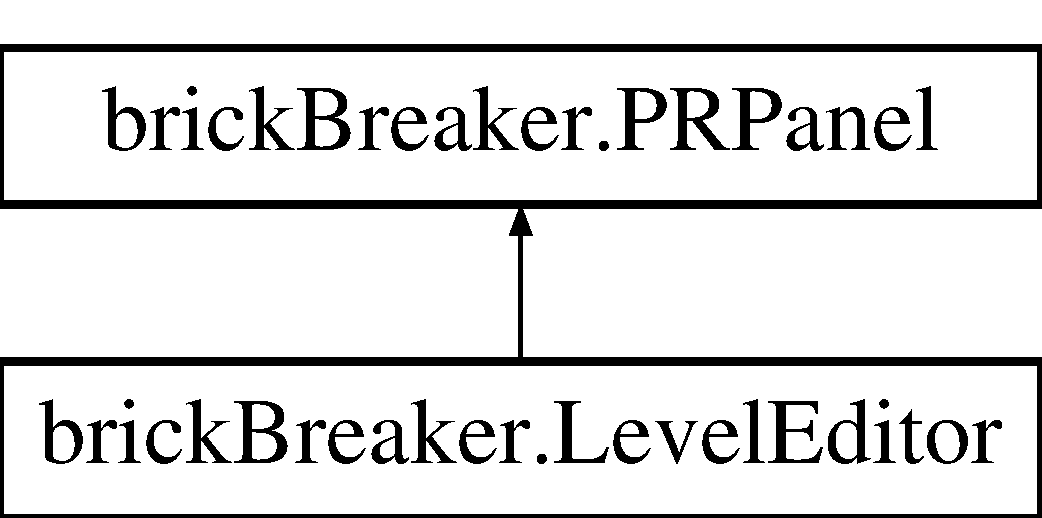
\includegraphics[height=2cm]{classbrick_breaker_1_1_level_editor}
\end{center}
\end{figure}
\subsection*{Public Member Functions}
\begin{DoxyCompactItemize}
\item 
\hyperlink{classbrick_breaker_1_1_level_editor_a7bd55dad6633ded18cb4fad7cf6bbeac}{LevelEditor} (\hyperlink{classbrick_breaker_1_1_start}{Start} s)
\item 
void \hyperlink{classbrick_breaker_1_1_level_editor_a5c1da01da393e14dbd38039bc457f713}{pause} ()
\item 
void \hyperlink{classbrick_breaker_1_1_level_editor_a25e9ea0a6e91f1848c3b76f66a238789}{resume} ()
\item 
void \hyperlink{classbrick_breaker_1_1_level_editor_aa38941ac69b2b38f472fd402d3e33e40}{stop} ()
\item 
void \hyperlink{classbrick_breaker_1_1_level_editor_ab2df7eb7b75f4e87b25c4b2d9422dc3d}{start} ()
\end{DoxyCompactItemize}
\subsection*{Static Public Attributes}
\begin{DoxyCompactItemize}
\item 
\hypertarget{classbrick_breaker_1_1_level_editor_ae0ab5f34aa01bae791c845b872c5fd4e}{
static final int {\bfseries PWIDTH} = 1000}
\label{classbrick_breaker_1_1_level_editor_ae0ab5f34aa01bae791c845b872c5fd4e}

\item 
\hypertarget{classbrick_breaker_1_1_level_editor_a790eed4b1962ef59c9be7b7456f5c1d5}{
static final int {\bfseries PHEIGHT} = 700}
\label{classbrick_breaker_1_1_level_editor_a790eed4b1962ef59c9be7b7456f5c1d5}

\item 
\hypertarget{classbrick_breaker_1_1_level_editor_a42f0d0ae33c6156c839f484227f46f8c}{
static final int {\bfseries BORDER} = 10}
\label{classbrick_breaker_1_1_level_editor_a42f0d0ae33c6156c839f484227f46f8c}

\item 
\hypertarget{classbrick_breaker_1_1_level_editor_a61ac04bbe7c6761edd08544444bca215}{
static final int {\bfseries ARENA\_\-WIDTH} = PWIDTH -\/ 2$\ast$BORDER}
\label{classbrick_breaker_1_1_level_editor_a61ac04bbe7c6761edd08544444bca215}

\item 
\hypertarget{classbrick_breaker_1_1_level_editor_ab2764a4a664527baa2bb4af2528da22b}{
static final int {\bfseries ARENA\_\-HEIGHT} = PHEIGHT -\/ 2$\ast$BORDER}
\label{classbrick_breaker_1_1_level_editor_ab2764a4a664527baa2bb4af2528da22b}

\end{DoxyCompactItemize}
\subsection*{Package Attributes}
\begin{DoxyCompactItemize}
\item 
\hypertarget{classbrick_breaker_1_1_level_editor_aaf99b1a788cb08d4a06f09e9bd3082ad}{
\hyperlink{classbrick_breaker_1_1_start}{Start} {\bfseries start}}
\label{classbrick_breaker_1_1_level_editor_aaf99b1a788cb08d4a06f09e9bd3082ad}

\item 
\hypertarget{classbrick_breaker_1_1_level_editor_a8ec9fae1671c98901c3b475380165394}{
int {\bfseries controlsWidth} = 200}
\label{classbrick_breaker_1_1_level_editor_a8ec9fae1671c98901c3b475380165394}

\item 
\hypertarget{classbrick_breaker_1_1_level_editor_afe941ba43411113e8839d2dd096b778d}{
int {\bfseries PWIDTHgrid} = PWIDTH -\/ controlsWidth}
\label{classbrick_breaker_1_1_level_editor_afe941ba43411113e8839d2dd096b778d}

\item 
\hypertarget{classbrick_breaker_1_1_level_editor_a8a906ab44e70601e3446f932db1bb751}{
int {\bfseries PHEIGHTgrid} = PHEIGHT}
\label{classbrick_breaker_1_1_level_editor_a8a906ab44e70601e3446f932db1bb751}

\item 
\hypertarget{classbrick_breaker_1_1_level_editor_ae0935f24f6b63be4738e299ed28786f0}{
int {\bfseries width} = PWIDTHgrid -\/ 2 $\ast$ BORDER}
\label{classbrick_breaker_1_1_level_editor_ae0935f24f6b63be4738e299ed28786f0}

\item 
\hypertarget{classbrick_breaker_1_1_level_editor_a769656f5f7b9751913a165d0292640d3}{
int {\bfseries height} = PHEIGHTgrid -\/ 2 $\ast$ BORDER}
\label{classbrick_breaker_1_1_level_editor_a769656f5f7b9751913a165d0292640d3}

\item 
\hypertarget{classbrick_breaker_1_1_level_editor_ae0a1406b008ab8782766cea7ce5a212e}{
int {\bfseries cornerX} = BORDER}
\label{classbrick_breaker_1_1_level_editor_ae0a1406b008ab8782766cea7ce5a212e}

\item 
\hypertarget{classbrick_breaker_1_1_level_editor_a11ad3d9dc458a90fa53308bc016e55e9}{
int {\bfseries cornerY} = BORDER}
\label{classbrick_breaker_1_1_level_editor_a11ad3d9dc458a90fa53308bc016e55e9}

\item 
\hypertarget{classbrick_breaker_1_1_level_editor_ad130c0330a5738a6544a72b87a0e0853}{
int {\bfseries minRows} = 1}
\label{classbrick_breaker_1_1_level_editor_ad130c0330a5738a6544a72b87a0e0853}

\item 
\hypertarget{classbrick_breaker_1_1_level_editor_a0ae8121ba8d6ec2a1a30e3974e8bd841}{
int {\bfseries maxRows} = 30}
\label{classbrick_breaker_1_1_level_editor_a0ae8121ba8d6ec2a1a30e3974e8bd841}

\item 
\hypertarget{classbrick_breaker_1_1_level_editor_a1586ac270f469e103231717d42745535}{
int {\bfseries minCols} = 1}
\label{classbrick_breaker_1_1_level_editor_a1586ac270f469e103231717d42745535}

\item 
\hypertarget{classbrick_breaker_1_1_level_editor_a58bc3f8b32530aeaf12cbe792c5b9d79}{
int {\bfseries maxCols} = 30}
\label{classbrick_breaker_1_1_level_editor_a58bc3f8b32530aeaf12cbe792c5b9d79}

\item 
\hypertarget{classbrick_breaker_1_1_level_editor_a4dd7aed8b876918fa98afeec65d56c46}{
int {\bfseries minPlayers} = 1}
\label{classbrick_breaker_1_1_level_editor_a4dd7aed8b876918fa98afeec65d56c46}

\item 
\hypertarget{classbrick_breaker_1_1_level_editor_a1cf297e13281a6717b9786509008e622}{
int {\bfseries maxPlayers} = 2}
\label{classbrick_breaker_1_1_level_editor_a1cf297e13281a6717b9786509008e622}

\item 
\hypertarget{classbrick_breaker_1_1_level_editor_afbeb48855365be9d655ae3075ef43a43}{
int {\bfseries r}}
\label{classbrick_breaker_1_1_level_editor_afbeb48855365be9d655ae3075ef43a43}

\item 
\hypertarget{classbrick_breaker_1_1_level_editor_a3990e01dab54bbd9254a242162591d7d}{
int {\bfseries c}}
\label{classbrick_breaker_1_1_level_editor_a3990e01dab54bbd9254a242162591d7d}

\item 
\hypertarget{classbrick_breaker_1_1_level_editor_a86fec16b38b4228d5d337d6816af783e}{
int {\bfseries players}}
\label{classbrick_breaker_1_1_level_editor_a86fec16b38b4228d5d337d6816af783e}

\item 
\hypertarget{classbrick_breaker_1_1_level_editor_aaa973070f553c1ce48909e55f407f3e2}{
String {\bfseries name} = \char`\"{}untitled-\/level\char`\"{}}
\label{classbrick_breaker_1_1_level_editor_aaa973070f553c1ce48909e55f407f3e2}

\item 
\hypertarget{classbrick_breaker_1_1_level_editor_a5470d46ed26f8f899c3beadcb8e7ba91}{
double {\bfseries boxHeight}}
\label{classbrick_breaker_1_1_level_editor_a5470d46ed26f8f899c3beadcb8e7ba91}

\item 
\hypertarget{classbrick_breaker_1_1_level_editor_a15df3c177f6c6a8cfdfddb43217133ee}{
double {\bfseries boxWidth}}
\label{classbrick_breaker_1_1_level_editor_a15df3c177f6c6a8cfdfddb43217133ee}

\item 
\hypertarget{classbrick_breaker_1_1_level_editor_a216bd897bcbc24ac22ccafb5fb585917}{
boolean {\bfseries gridGenerated} = false}
\label{classbrick_breaker_1_1_level_editor_a216bd897bcbc24ac22ccafb5fb585917}

\item 
\hypertarget{classbrick_breaker_1_1_level_editor_ac1b0001de7a7725509ebbcaed5041dae}{
boolean {\bfseries mouseDown}}
\label{classbrick_breaker_1_1_level_editor_ac1b0001de7a7725509ebbcaed5041dae}

\item 
\hypertarget{classbrick_breaker_1_1_level_editor_abd64bc7df827fdcdf9c4b2ca910c44bd}{
int {\bfseries mx1} = -\/1}
\label{classbrick_breaker_1_1_level_editor_abd64bc7df827fdcdf9c4b2ca910c44bd}

\item 
\hypertarget{classbrick_breaker_1_1_level_editor_a590c966326e6c45478b08dbea4c3b475}{
int {\bfseries my1} = -\/1}
\label{classbrick_breaker_1_1_level_editor_a590c966326e6c45478b08dbea4c3b475}

\item 
\hypertarget{classbrick_breaker_1_1_level_editor_a8e5b5bd4890c69a2119460acfd9e06f0}{
int {\bfseries mx2} = -\/1}
\label{classbrick_breaker_1_1_level_editor_a8e5b5bd4890c69a2119460acfd9e06f0}

\item 
\hypertarget{classbrick_breaker_1_1_level_editor_a21c4714ac188f89e76977af9ee4062ba}{
int {\bfseries my2} = -\/1}
\label{classbrick_breaker_1_1_level_editor_a21c4714ac188f89e76977af9ee4062ba}

\item 
\hypertarget{classbrick_breaker_1_1_level_editor_af0340dfeb06e0e42050ee8b532acbfad}{
boolean\mbox{[}$\,$\mbox{]}\mbox{[}$\,$\mbox{]} {\bfseries blocks}}
\label{classbrick_breaker_1_1_level_editor_af0340dfeb06e0e42050ee8b532acbfad}

\item 
\hypertarget{classbrick_breaker_1_1_level_editor_ad680658f88e1d468ef4b377836189bc5}{
\hyperlink{classbrick_breaker_1_1_brick}{Brick}\mbox{[}$\,$\mbox{]}\mbox{[}$\,$\mbox{]} {\bfseries bricks}}
\label{classbrick_breaker_1_1_level_editor_ad680658f88e1d468ef4b377836189bc5}

\end{DoxyCompactItemize}


\subsection{Detailed Description}
\begin{DoxyAuthor}{Author}
Robert Nishihara 
\end{DoxyAuthor}
\begin{DoxyVersion}{Version}
5/02/10 
\end{DoxyVersion}


\subsection{Constructor \& Destructor Documentation}
\hypertarget{classbrick_breaker_1_1_level_editor_a7bd55dad6633ded18cb4fad7cf6bbeac}{
\index{brickBreaker::LevelEditor@{brickBreaker::LevelEditor}!LevelEditor@{LevelEditor}}
\index{LevelEditor@{LevelEditor}!brickBreaker::LevelEditor@{brickBreaker::LevelEditor}}
\subsubsection[{LevelEditor}]{\setlength{\rightskip}{0pt plus 5cm}brickBreaker.LevelEditor.LevelEditor ({\bf Start} {\em s})}}
\label{classbrick_breaker_1_1_level_editor_a7bd55dad6633ded18cb4fad7cf6bbeac}
Constructor


\begin{DoxyParams}{Parameters}
\item[{\em s}]The JFrame which \hyperlink{classbrick_breaker_1_1_level_editor}{LevelEditor} is a part of \end{DoxyParams}


\subsection{Member Function Documentation}
\hypertarget{classbrick_breaker_1_1_level_editor_a5c1da01da393e14dbd38039bc457f713}{
\index{brickBreaker::LevelEditor@{brickBreaker::LevelEditor}!pause@{pause}}
\index{pause@{pause}!brickBreaker::LevelEditor@{brickBreaker::LevelEditor}}
\subsubsection[{pause}]{\setlength{\rightskip}{0pt plus 5cm}void brickBreaker.LevelEditor.pause ()}}
\label{classbrick_breaker_1_1_level_editor_a5c1da01da393e14dbd38039bc457f713}
Pauses \hyperlink{classbrick_breaker_1_1_level_editor}{LevelEditor} 

Reimplemented from \hyperlink{classbrick_breaker_1_1_p_r_panel_a0868e501fc5599973492e6f0c53da920}{brickBreaker.PRPanel}.

\hypertarget{classbrick_breaker_1_1_level_editor_a25e9ea0a6e91f1848c3b76f66a238789}{
\index{brickBreaker::LevelEditor@{brickBreaker::LevelEditor}!resume@{resume}}
\index{resume@{resume}!brickBreaker::LevelEditor@{brickBreaker::LevelEditor}}
\subsubsection[{resume}]{\setlength{\rightskip}{0pt plus 5cm}void brickBreaker.LevelEditor.resume ()}}
\label{classbrick_breaker_1_1_level_editor_a25e9ea0a6e91f1848c3b76f66a238789}
Resumes \hyperlink{classbrick_breaker_1_1_level_editor}{LevelEditor} 

Reimplemented from \hyperlink{classbrick_breaker_1_1_p_r_panel_ac9aadc88543f9032a27f3eb2b8ea908b}{brickBreaker.PRPanel}.

\hypertarget{classbrick_breaker_1_1_level_editor_ab2df7eb7b75f4e87b25c4b2d9422dc3d}{
\index{brickBreaker::LevelEditor@{brickBreaker::LevelEditor}!start@{start}}
\index{start@{start}!brickBreaker::LevelEditor@{brickBreaker::LevelEditor}}
\subsubsection[{start}]{\setlength{\rightskip}{0pt plus 5cm}void brickBreaker.LevelEditor.start ()}}
\label{classbrick_breaker_1_1_level_editor_ab2df7eb7b75f4e87b25c4b2d9422dc3d}
Starts \hyperlink{classbrick_breaker_1_1_level_editor}{LevelEditor} and sets text fields to their default values 

Reimplemented from \hyperlink{classbrick_breaker_1_1_p_r_panel_a94e190e70d6aa937068cbf5e8cff523e}{brickBreaker.PRPanel}.

\hypertarget{classbrick_breaker_1_1_level_editor_aa38941ac69b2b38f472fd402d3e33e40}{
\index{brickBreaker::LevelEditor@{brickBreaker::LevelEditor}!stop@{stop}}
\index{stop@{stop}!brickBreaker::LevelEditor@{brickBreaker::LevelEditor}}
\subsubsection[{stop}]{\setlength{\rightskip}{0pt plus 5cm}void brickBreaker.LevelEditor.stop ()}}
\label{classbrick_breaker_1_1_level_editor_aa38941ac69b2b38f472fd402d3e33e40}
Stops \hyperlink{classbrick_breaker_1_1_level_editor}{LevelEditor} 

Reimplemented from \hyperlink{classbrick_breaker_1_1_p_r_panel_ad077fab978f84663f366a6fdde5efe6c}{brickBreaker.PRPanel}.



The documentation for this class was generated from the following file:\begin{DoxyCompactItemize}
\item 
src/game/brickBreaker/LevelEditor.java\end{DoxyCompactItemize}

\hypertarget{classbrick_breaker_1_1_level_initializer}{
\section{brickBreaker.LevelInitializer Class Reference}
\label{classbrick_breaker_1_1_level_initializer}\index{brickBreaker::LevelInitializer@{brickBreaker::LevelInitializer}}
}
\subsection*{Static Public Member Functions}
\begin{DoxyCompactItemize}
\item 
\hypertarget{classbrick_breaker_1_1_level_initializer_afacc07e5171f482c78534f1d5ac68675}{
static \hyperlink{classbrick_breaker_1_1_level}{Level}\mbox{[}$\,$\mbox{]} {\bfseries generateLevels} (int numPlayers)}
\label{classbrick_breaker_1_1_level_initializer_afacc07e5171f482c78534f1d5ac68675}

\item 
\hypertarget{classbrick_breaker_1_1_level_initializer_ac33a0530b0b29f684b1d0606e93446a2}{
static \hyperlink{classbrick_breaker_1_1_level}{Level}\mbox{[}$\,$\mbox{]} {\bfseries generateOnePlayer} ()}
\label{classbrick_breaker_1_1_level_initializer_ac33a0530b0b29f684b1d0606e93446a2}

\item 
\hypertarget{classbrick_breaker_1_1_level_initializer_a16b18591cd2d4ab4a27aae14f2f3cc14}{
static \hyperlink{classbrick_breaker_1_1_level}{Level}\mbox{[}$\,$\mbox{]} {\bfseries generateTwoPlayers} ()}
\label{classbrick_breaker_1_1_level_initializer_a16b18591cd2d4ab4a27aae14f2f3cc14}

\item 
\hypertarget{classbrick_breaker_1_1_level_initializer_afb5066708c4693653fff665fa9974469}{
static \hyperlink{classbrick_breaker_1_1_level}{Level}\mbox{[}$\,$\mbox{]} {\bfseries generateFourPlayers} ()}
\label{classbrick_breaker_1_1_level_initializer_afb5066708c4693653fff665fa9974469}

\end{DoxyCompactItemize}
\subsection*{Static Public Attributes}
\begin{DoxyCompactItemize}
\item 
\hypertarget{classbrick_breaker_1_1_level_initializer_abf93f8503b568500ca05a1c6b7189788}{
static final double {\bfseries pi} = Math.PI}
\label{classbrick_breaker_1_1_level_initializer_abf93f8503b568500ca05a1c6b7189788}

\item 
\hypertarget{classbrick_breaker_1_1_level_initializer_a725f415e02e42e2d8cf49e83ebd245ef}{
static final int {\bfseries width} = GamePanel.ARENA\_\-WIDTH}
\label{classbrick_breaker_1_1_level_initializer_a725f415e02e42e2d8cf49e83ebd245ef}

\item 
\hypertarget{classbrick_breaker_1_1_level_initializer_a7bf5b50b3f52b878e4071b64b75f530e}{
static final int {\bfseries height} = GamePanel.ARENA\_\-HEIGHT}
\label{classbrick_breaker_1_1_level_initializer_a7bf5b50b3f52b878e4071b64b75f530e}

\end{DoxyCompactItemize}


\subsection{Detailed Description}
Includes methods for initializing a number of default levels for 1, 2 or 4 players 

The documentation for this class was generated from the following file:\begin{DoxyCompactItemize}
\item 
src/game/brickBreaker/LevelInitializer.java\end{DoxyCompactItemize}

\hypertarget{classbrick_breaker_1_1_level_player}{
\section{brickBreaker.LevelPlayer Class Reference}
\label{classbrick_breaker_1_1_level_player}\index{brickBreaker::LevelPlayer@{brickBreaker::LevelPlayer}}
}
\subsection*{Public Member Functions}
\begin{DoxyCompactItemize}
\item 
\hyperlink{classbrick_breaker_1_1_level_player_a34f8b2db5684239038d4b5f33d7c93f6}{LevelPlayer} (\hyperlink{classbrick_breaker_1_1_level}{Level} lev)
\item 
int \hyperlink{classbrick_breaker_1_1_level_player_ad141c01fb30f6982c5b7932dd8ca901a}{update} ()
\item 
boolean \hyperlink{classbrick_breaker_1_1_level_player_aa5069116c7e903a1cf8d6663260905b2}{ballsInBounds} ()
\item 
boolean \hyperlink{classbrick_breaker_1_1_level_player_a298ae45b06799f0299d4b518075b9599}{isFilled} (int x, int y)
\item 
int \hyperlink{classbrick_breaker_1_1_level_player_a6aa16018bbba510ef65b6d43baaf8dc3}{removeBrick} (int x, int y, \hyperlink{classbrick_breaker_1_1_ball}{Ball} b)
\item 
int \hyperlink{classbrick_breaker_1_1_level_player_a0faa4b97a3ae3d8f473a5b70de9ab45b}{checkCollision} (\hyperlink{classbrick_breaker_1_1_ball}{Ball} b)
\item 
boolean \hyperlink{classbrick_breaker_1_1_level_player_a952e8b565a2c36ac471f7ab020972294}{cleared} ()
\item 
boolean \hyperlink{classbrick_breaker_1_1_level_player_ad4ab8305c27d7ee5a1c4a05488705a53}{racketLeft} ()
\item 
boolean \hyperlink{classbrick_breaker_1_1_level_player_a95c24168beb56156276b636954f210bc}{racketRight} ()
\item 
boolean \hyperlink{classbrick_breaker_1_1_level_player_ae31f4ca8b38e813587e795d681edfb0d}{racketTop} ()
\item 
boolean \hyperlink{classbrick_breaker_1_1_level_player_a6a7980415c6fed32a9f6c9271bae6220}{racketBottom} ()
\item 
void \hyperlink{classbrick_breaker_1_1_level_player_ae54384ce113e96099dd14d73acd7de5e}{drawComponents} (Graphics g)
\item 
void \hyperlink{classbrick_breaker_1_1_level_player_a1ebfab24bc0e7e7e6851f7856e486d8d}{keyPressed} (int code)
\item 
void \hyperlink{classbrick_breaker_1_1_level_player_a32dd9508bac5135b7f2706b807ada71e}{keyReleased} (int code)
\item 
\hypertarget{classbrick_breaker_1_1_level_player_a732aa75e9304df978a19452b95b6ee87}{
\hyperlink{classbrick_breaker_1_1_level}{Level} {\bfseries getLevel} ()}
\label{classbrick_breaker_1_1_level_player_a732aa75e9304df978a19452b95b6ee87}

\end{DoxyCompactItemize}
\subsection*{Static Public Attributes}
\begin{DoxyCompactItemize}
\item 
\hypertarget{classbrick_breaker_1_1_level_player_a0fabd8254a778679106f0817ec18d4d8}{
static int {\bfseries WIDTH}}
\label{classbrick_breaker_1_1_level_player_a0fabd8254a778679106f0817ec18d4d8}

\item 
\hypertarget{classbrick_breaker_1_1_level_player_a78ba1a2042a37d401a70998c49030b7c}{
static int {\bfseries HEIGHT}}
\label{classbrick_breaker_1_1_level_player_a78ba1a2042a37d401a70998c49030b7c}

\end{DoxyCompactItemize}


\subsection{Constructor \& Destructor Documentation}
\hypertarget{classbrick_breaker_1_1_level_player_a34f8b2db5684239038d4b5f33d7c93f6}{
\index{brickBreaker::LevelPlayer@{brickBreaker::LevelPlayer}!LevelPlayer@{LevelPlayer}}
\index{LevelPlayer@{LevelPlayer}!brickBreaker::LevelPlayer@{brickBreaker::LevelPlayer}}
\subsubsection[{LevelPlayer}]{\setlength{\rightskip}{0pt plus 5cm}brickBreaker.LevelPlayer.LevelPlayer ({\bf Level} {\em lev})}}
\label{classbrick_breaker_1_1_level_player_a34f8b2db5684239038d4b5f33d7c93f6}
Constructor 
\begin{DoxyParams}{Parameters}
\item[{\em lev}]The \hyperlink{classbrick_breaker_1_1_level}{Level} object containing the components used by this class \end{DoxyParams}


\subsection{Member Function Documentation}
\hypertarget{classbrick_breaker_1_1_level_player_aa5069116c7e903a1cf8d6663260905b2}{
\index{brickBreaker::LevelPlayer@{brickBreaker::LevelPlayer}!ballsInBounds@{ballsInBounds}}
\index{ballsInBounds@{ballsInBounds}!brickBreaker::LevelPlayer@{brickBreaker::LevelPlayer}}
\subsubsection[{ballsInBounds}]{\setlength{\rightskip}{0pt plus 5cm}boolean brickBreaker.LevelPlayer.ballsInBounds ()}}
\label{classbrick_breaker_1_1_level_player_aa5069116c7e903a1cf8d6663260905b2}
Tests whether all balls are still in play. \begin{DoxyReturn}{Returns}
Returns true if all the balls are still in bounds 
\end{DoxyReturn}
\hypertarget{classbrick_breaker_1_1_level_player_a0faa4b97a3ae3d8f473a5b70de9ab45b}{
\index{brickBreaker::LevelPlayer@{brickBreaker::LevelPlayer}!checkCollision@{checkCollision}}
\index{checkCollision@{checkCollision}!brickBreaker::LevelPlayer@{brickBreaker::LevelPlayer}}
\subsubsection[{checkCollision}]{\setlength{\rightskip}{0pt plus 5cm}int brickBreaker.LevelPlayer.checkCollision ({\bf Ball} {\em b})}}
\label{classbrick_breaker_1_1_level_player_a0faa4b97a3ae3d8f473a5b70de9ab45b}
Checks whether the given ball is colliding with any brick, and updates the bricks if needed.


\begin{DoxyParams}{Parameters}
\item[{\em b}]The ball to be tested \end{DoxyParams}
\begin{DoxyReturn}{Returns}
Returns the number of points earned (zero if no bricks were removed) 
\end{DoxyReturn}
\hypertarget{classbrick_breaker_1_1_level_player_a952e8b565a2c36ac471f7ab020972294}{
\index{brickBreaker::LevelPlayer@{brickBreaker::LevelPlayer}!cleared@{cleared}}
\index{cleared@{cleared}!brickBreaker::LevelPlayer@{brickBreaker::LevelPlayer}}
\subsubsection[{cleared}]{\setlength{\rightskip}{0pt plus 5cm}boolean brickBreaker.LevelPlayer.cleared ()}}
\label{classbrick_breaker_1_1_level_player_a952e8b565a2c36ac471f7ab020972294}
Tests whether all of the bricks have been cleared from the level. \begin{DoxyReturn}{Returns}
Returns true if all bricks have been removed (ignoring permanent bricks) 
\end{DoxyReturn}
\hypertarget{classbrick_breaker_1_1_level_player_ae54384ce113e96099dd14d73acd7de5e}{
\index{brickBreaker::LevelPlayer@{brickBreaker::LevelPlayer}!drawComponents@{drawComponents}}
\index{drawComponents@{drawComponents}!brickBreaker::LevelPlayer@{brickBreaker::LevelPlayer}}
\subsubsection[{drawComponents}]{\setlength{\rightskip}{0pt plus 5cm}void brickBreaker.LevelPlayer.drawComponents (Graphics {\em g})}}
\label{classbrick_breaker_1_1_level_player_ae54384ce113e96099dd14d73acd7de5e}
Draws all of the level components on the screen. 
\begin{DoxyParams}{Parameters}
\item[{\em g}]Graphics object to draw with \end{DoxyParams}
\hypertarget{classbrick_breaker_1_1_level_player_a298ae45b06799f0299d4b518075b9599}{
\index{brickBreaker::LevelPlayer@{brickBreaker::LevelPlayer}!isFilled@{isFilled}}
\index{isFilled@{isFilled}!brickBreaker::LevelPlayer@{brickBreaker::LevelPlayer}}
\subsubsection[{isFilled}]{\setlength{\rightskip}{0pt plus 5cm}boolean brickBreaker.LevelPlayer.isFilled (int {\em x}, \/  int {\em y})}}
\label{classbrick_breaker_1_1_level_player_a298ae45b06799f0299d4b518075b9599}
Tests whether the position \mbox{[}x\mbox{]}\mbox{[}y\mbox{]} (in the 2d array of bricks) is occupied by a brick.


\begin{DoxyParams}{Parameters}
\item[{\em x}]The x-\/coordinate of the position in the brick grid \item[{\em y}]The y-\/coordinate of the position in the brick grid \end{DoxyParams}
\begin{DoxyReturn}{Returns}
Returns true if the given position is occupied by a brick, false if it is empty 
\end{DoxyReturn}
\hypertarget{classbrick_breaker_1_1_level_player_a1ebfab24bc0e7e7e6851f7856e486d8d}{
\index{brickBreaker::LevelPlayer@{brickBreaker::LevelPlayer}!keyPressed@{keyPressed}}
\index{keyPressed@{keyPressed}!brickBreaker::LevelPlayer@{brickBreaker::LevelPlayer}}
\subsubsection[{keyPressed}]{\setlength{\rightskip}{0pt plus 5cm}void brickBreaker.LevelPlayer.keyPressed (int {\em code})}}
\label{classbrick_breaker_1_1_level_player_a1ebfab24bc0e7e7e6851f7856e486d8d}
Actions to be performed when a key is pressed 
\begin{DoxyParams}{Parameters}
\item[{\em code}]Int key code \end{DoxyParams}
\hypertarget{classbrick_breaker_1_1_level_player_a32dd9508bac5135b7f2706b807ada71e}{
\index{brickBreaker::LevelPlayer@{brickBreaker::LevelPlayer}!keyReleased@{keyReleased}}
\index{keyReleased@{keyReleased}!brickBreaker::LevelPlayer@{brickBreaker::LevelPlayer}}
\subsubsection[{keyReleased}]{\setlength{\rightskip}{0pt plus 5cm}void brickBreaker.LevelPlayer.keyReleased (int {\em code})}}
\label{classbrick_breaker_1_1_level_player_a32dd9508bac5135b7f2706b807ada71e}
Actions to be performed when a key is released 
\begin{DoxyParams}{Parameters}
\item[{\em code}]Int key code \end{DoxyParams}
\hypertarget{classbrick_breaker_1_1_level_player_a6a7980415c6fed32a9f6c9271bae6220}{
\index{brickBreaker::LevelPlayer@{brickBreaker::LevelPlayer}!racketBottom@{racketBottom}}
\index{racketBottom@{racketBottom}!brickBreaker::LevelPlayer@{brickBreaker::LevelPlayer}}
\subsubsection[{racketBottom}]{\setlength{\rightskip}{0pt plus 5cm}boolean brickBreaker.LevelPlayer.racketBottom ()}}
\label{classbrick_breaker_1_1_level_player_a6a7980415c6fed32a9f6c9271bae6220}
Returns true if there is a racket on the bottom of the screen \hypertarget{classbrick_breaker_1_1_level_player_ad4ab8305c27d7ee5a1c4a05488705a53}{
\index{brickBreaker::LevelPlayer@{brickBreaker::LevelPlayer}!racketLeft@{racketLeft}}
\index{racketLeft@{racketLeft}!brickBreaker::LevelPlayer@{brickBreaker::LevelPlayer}}
\subsubsection[{racketLeft}]{\setlength{\rightskip}{0pt plus 5cm}boolean brickBreaker.LevelPlayer.racketLeft ()}}
\label{classbrick_breaker_1_1_level_player_ad4ab8305c27d7ee5a1c4a05488705a53}
Returns true if there is a racket on the left side of the screen \hypertarget{classbrick_breaker_1_1_level_player_a95c24168beb56156276b636954f210bc}{
\index{brickBreaker::LevelPlayer@{brickBreaker::LevelPlayer}!racketRight@{racketRight}}
\index{racketRight@{racketRight}!brickBreaker::LevelPlayer@{brickBreaker::LevelPlayer}}
\subsubsection[{racketRight}]{\setlength{\rightskip}{0pt plus 5cm}boolean brickBreaker.LevelPlayer.racketRight ()}}
\label{classbrick_breaker_1_1_level_player_a95c24168beb56156276b636954f210bc}
Returns true if there is a racket on the right side of the screen \hypertarget{classbrick_breaker_1_1_level_player_ae31f4ca8b38e813587e795d681edfb0d}{
\index{brickBreaker::LevelPlayer@{brickBreaker::LevelPlayer}!racketTop@{racketTop}}
\index{racketTop@{racketTop}!brickBreaker::LevelPlayer@{brickBreaker::LevelPlayer}}
\subsubsection[{racketTop}]{\setlength{\rightskip}{0pt plus 5cm}boolean brickBreaker.LevelPlayer.racketTop ()}}
\label{classbrick_breaker_1_1_level_player_ae31f4ca8b38e813587e795d681edfb0d}
Returns true if there is a racket on the top of the screen \hypertarget{classbrick_breaker_1_1_level_player_a6aa16018bbba510ef65b6d43baaf8dc3}{
\index{brickBreaker::LevelPlayer@{brickBreaker::LevelPlayer}!removeBrick@{removeBrick}}
\index{removeBrick@{removeBrick}!brickBreaker::LevelPlayer@{brickBreaker::LevelPlayer}}
\subsubsection[{removeBrick}]{\setlength{\rightskip}{0pt plus 5cm}int brickBreaker.LevelPlayer.removeBrick (int {\em x}, \/  int {\em y}, \/  {\bf Ball} {\em b})}}
\label{classbrick_breaker_1_1_level_player_a6aa16018bbba510ef65b6d43baaf8dc3}
Removes the box at \mbox{[}x\mbox{]}\mbox{[}y\mbox{]} in the array of bricks.


\begin{DoxyParams}{Parameters}
\item[{\em x}]The x-\/coordinate of the position in the brick grid \item[{\em y}]The y-\/coordinate of the position in the brick grid \item[{\em b}]The ball which just bounced against the brick \end{DoxyParams}
\begin{DoxyReturn}{Returns}
Returns the number of points earned by removing this brick 
\end{DoxyReturn}
\hypertarget{classbrick_breaker_1_1_level_player_ad141c01fb30f6982c5b7932dd8ca901a}{
\index{brickBreaker::LevelPlayer@{brickBreaker::LevelPlayer}!update@{update}}
\index{update@{update}!brickBreaker::LevelPlayer@{brickBreaker::LevelPlayer}}
\subsubsection[{update}]{\setlength{\rightskip}{0pt plus 5cm}int brickBreaker.LevelPlayer.update ()}}
\label{classbrick_breaker_1_1_level_player_ad141c01fb30f6982c5b7932dd8ca901a}
Updates the components in the level and returns the score earned. \begin{DoxyReturn}{Returns}
Returns the number of points earned in this timestep 
\end{DoxyReturn}


The documentation for this class was generated from the following file:\begin{DoxyCompactItemize}
\item 
game/brickBreaker/\hyperlink{_level_player_8java}{LevelPlayer.java}\end{DoxyCompactItemize}

\hypertarget{classbrick_breaker_1_1local_1_1_local_data_service}{
\section{brickBreaker.local.LocalDataService Class Reference}
\label{classbrick_breaker_1_1local_1_1_local_data_service}\index{brickBreaker::local::LocalDataService@{brickBreaker::local::LocalDataService}}
}
\subsection*{Static Public Member Functions}
\begin{DoxyCompactItemize}
\item 
static void \hyperlink{classbrick_breaker_1_1local_1_1_local_data_service_a01f5a08e38cd865add34f24a7634cf38}{saveLevel} (\hyperlink{classbrick_breaker_1_1_level}{Level} level, String filename)  throws FilesystemFailureException 
\item 
static BiMap$<$ String, \hyperlink{classbrick_breaker_1_1_level}{Level} $>$ \hyperlink{classbrick_breaker_1_1local_1_1_local_data_service_a498aa81a0d3ac82f0818dd9e3df6ee3d}{loadAllLevelsFromDisk} ()  throws FilesystemFailureException 
\item 
static String \hyperlink{classbrick_breaker_1_1local_1_1_local_data_service_a81493703f640a10d1b66fe2110f01d48}{calculateHash} (\hyperlink{classbrick_breaker_1_1_level}{Level} level)
\end{DoxyCompactItemize}


\subsection{Detailed Description}
This class provides methods for persisting and loading levels by using the local filesystem.

\begin{DoxyAuthor}{Author}
Abraham Lin 
\end{DoxyAuthor}


\subsection{Member Function Documentation}
\hypertarget{classbrick_breaker_1_1local_1_1_local_data_service_a81493703f640a10d1b66fe2110f01d48}{
\index{brickBreaker::local::LocalDataService@{brickBreaker::local::LocalDataService}!calculateHash@{calculateHash}}
\index{calculateHash@{calculateHash}!brickBreaker::local::LocalDataService@{brickBreaker::local::LocalDataService}}
\subsubsection[{calculateHash}]{\setlength{\rightskip}{0pt plus 5cm}static String brickBreaker.local.LocalDataService.calculateHash ({\bf Level} {\em level})\hspace{0.3cm}{\ttfamily  \mbox{[}static\mbox{]}}}}
\label{classbrick_breaker_1_1local_1_1_local_data_service_a81493703f640a10d1b66fe2110f01d48}
Calculates the MD5 hash for the provided level.


\begin{DoxyParams}{Parameters}
\item[{\em level}]the level \end{DoxyParams}
\begin{DoxyReturn}{Returns}
the MD5 hash of the level 
\end{DoxyReturn}
\hypertarget{classbrick_breaker_1_1local_1_1_local_data_service_a498aa81a0d3ac82f0818dd9e3df6ee3d}{
\index{brickBreaker::local::LocalDataService@{brickBreaker::local::LocalDataService}!loadAllLevelsFromDisk@{loadAllLevelsFromDisk}}
\index{loadAllLevelsFromDisk@{loadAllLevelsFromDisk}!brickBreaker::local::LocalDataService@{brickBreaker::local::LocalDataService}}
\subsubsection[{loadAllLevelsFromDisk}]{\setlength{\rightskip}{0pt plus 5cm}static BiMap$<$String, {\bf Level}$>$ brickBreaker.local.LocalDataService.loadAllLevelsFromDisk ()  throws {\bf FilesystemFailureException} \hspace{0.3cm}{\ttfamily  \mbox{[}static\mbox{]}}}}
\label{classbrick_breaker_1_1local_1_1_local_data_service_a498aa81a0d3ac82f0818dd9e3df6ee3d}
Loads all existing levels from the filesystem.

\begin{DoxyReturn}{Returns}
a list of all loaded levels
\end{DoxyReturn}

\begin{DoxyExceptions}{Exceptions}
\item[{\em \hyperlink{classbrick_breaker_1_1local_1_1_filesystem_failure_exception}{FilesystemFailureException}}]if any errors occur while attempting the operation \end{DoxyExceptions}
\hypertarget{classbrick_breaker_1_1local_1_1_local_data_service_a01f5a08e38cd865add34f24a7634cf38}{
\index{brickBreaker::local::LocalDataService@{brickBreaker::local::LocalDataService}!saveLevel@{saveLevel}}
\index{saveLevel@{saveLevel}!brickBreaker::local::LocalDataService@{brickBreaker::local::LocalDataService}}
\subsubsection[{saveLevel}]{\setlength{\rightskip}{0pt plus 5cm}static void brickBreaker.local.LocalDataService.saveLevel ({\bf Level} {\em level}, \/  String {\em filename})  throws {\bf FilesystemFailureException} \hspace{0.3cm}{\ttfamily  \mbox{[}static\mbox{]}}}}
\label{classbrick_breaker_1_1local_1_1_local_data_service_a01f5a08e38cd865add34f24a7634cf38}
Saves the specified level using the provided filename.


\begin{DoxyParams}{Parameters}
\item[{\em level}]the level to save \item[{\em filename}]the filename for the level file\end{DoxyParams}

\begin{DoxyExceptions}{Exceptions}
\item[{\em \hyperlink{classbrick_breaker_1_1local_1_1_filesystem_failure_exception}{FilesystemFailureException}}]if any errors occur while attempting the operation \end{DoxyExceptions}


The documentation for this class was generated from the following file:\begin{DoxyCompactItemize}
\item 
src/game/brickBreaker/local/LocalDataService.java\end{DoxyCompactItemize}

\hypertarget{classbrick_breaker_1_1web_1_1_online_level}{
\section{brickBreaker.web.OnlineLevel Class Reference}
\label{classbrick_breaker_1_1web_1_1_online_level}\index{brickBreaker::web::OnlineLevel@{brickBreaker::web::OnlineLevel}}
}
\subsection*{Public Member Functions}
\begin{DoxyCompactItemize}
\item 
\hyperlink{classbrick_breaker_1_1web_1_1_online_level_a3d31cb97e69deb979c586a78872beac5}{OnlineLevel} (String levelID, String title)
\item 
String \hyperlink{classbrick_breaker_1_1web_1_1_online_level_a265cd345985cde1aa244cb739445bbc3}{getLevelID} ()
\item 
String \hyperlink{classbrick_breaker_1_1web_1_1_online_level_a0a23b746281c6b60e88dab532ab77df4}{getTitle} ()
\end{DoxyCompactItemize}


\subsection{Detailed Description}
This class provides a representation of a remotely available level with a unique identifier and title.

\begin{DoxyAuthor}{Author}
Abraham Lin 
\end{DoxyAuthor}


\subsection{Constructor \& Destructor Documentation}
\hypertarget{classbrick_breaker_1_1web_1_1_online_level_a3d31cb97e69deb979c586a78872beac5}{
\index{brickBreaker::web::OnlineLevel@{brickBreaker::web::OnlineLevel}!OnlineLevel@{OnlineLevel}}
\index{OnlineLevel@{OnlineLevel}!brickBreaker::web::OnlineLevel@{brickBreaker::web::OnlineLevel}}
\subsubsection[{OnlineLevel}]{\setlength{\rightskip}{0pt plus 5cm}brickBreaker.web.OnlineLevel.OnlineLevel (String {\em levelID}, \/  String {\em title})}}
\label{classbrick_breaker_1_1web_1_1_online_level_a3d31cb97e69deb979c586a78872beac5}
Constructs a level representation with the given unique identifier and title.


\begin{DoxyParams}{Parameters}
\item[{\em levelID}]the unique identifier \item[{\em title}]the title \end{DoxyParams}


\subsection{Member Function Documentation}
\hypertarget{classbrick_breaker_1_1web_1_1_online_level_a265cd345985cde1aa244cb739445bbc3}{
\index{brickBreaker::web::OnlineLevel@{brickBreaker::web::OnlineLevel}!getLevelID@{getLevelID}}
\index{getLevelID@{getLevelID}!brickBreaker::web::OnlineLevel@{brickBreaker::web::OnlineLevel}}
\subsubsection[{getLevelID}]{\setlength{\rightskip}{0pt plus 5cm}String brickBreaker.web.OnlineLevel.getLevelID ()}}
\label{classbrick_breaker_1_1web_1_1_online_level_a265cd345985cde1aa244cb739445bbc3}
Returns the unique identifier of this level representation.

\begin{DoxyReturn}{Returns}
the unique identifier 
\end{DoxyReturn}
\hypertarget{classbrick_breaker_1_1web_1_1_online_level_a0a23b746281c6b60e88dab532ab77df4}{
\index{brickBreaker::web::OnlineLevel@{brickBreaker::web::OnlineLevel}!getTitle@{getTitle}}
\index{getTitle@{getTitle}!brickBreaker::web::OnlineLevel@{brickBreaker::web::OnlineLevel}}
\subsubsection[{getTitle}]{\setlength{\rightskip}{0pt plus 5cm}String brickBreaker.web.OnlineLevel.getTitle ()}}
\label{classbrick_breaker_1_1web_1_1_online_level_a0a23b746281c6b60e88dab532ab77df4}
Returns the title associated with this level representation.

\begin{DoxyReturn}{Returns}
the title 
\end{DoxyReturn}


The documentation for this class was generated from the following file:\begin{DoxyCompactItemize}
\item 
src/game/brickBreaker/web/OnlineLevel.java\end{DoxyCompactItemize}

\hypertarget{classbrick_breaker_1_1_password_box}{
\section{brickBreaker.PasswordBox Class Reference}
\label{classbrick_breaker_1_1_password_box}\index{brickBreaker::PasswordBox@{brickBreaker::PasswordBox}}
}
\subsection*{Public Member Functions}
\begin{DoxyCompactItemize}
\item 
boolean \hyperlink{classbrick_breaker_1_1_password_box_a286ea1727bf1fbaeba6ba928d0779526}{checkLogin} ()
\item 
boolean \hyperlink{classbrick_breaker_1_1_password_box_a88b47539fc6a2f7b7e51a8258d5821de}{checkSkipped} ()
\end{DoxyCompactItemize}


\subsection{Detailed Description}
\begin{DoxyAuthor}{Author}
Jacob 
\end{DoxyAuthor}


\subsection{Member Function Documentation}
\hypertarget{classbrick_breaker_1_1_password_box_a286ea1727bf1fbaeba6ba928d0779526}{
\index{brickBreaker::PasswordBox@{brickBreaker::PasswordBox}!checkLogin@{checkLogin}}
\index{checkLogin@{checkLogin}!brickBreaker::PasswordBox@{brickBreaker::PasswordBox}}
\subsubsection[{checkLogin}]{\setlength{\rightskip}{0pt plus 5cm}boolean brickBreaker.PasswordBox.checkLogin ()}}
\label{classbrick_breaker_1_1_password_box_a286ea1727bf1fbaeba6ba928d0779526}
Check if user is logged in

\begin{DoxyReturn}{Returns}
True if user is logged in, else false 
\end{DoxyReturn}
\hypertarget{classbrick_breaker_1_1_password_box_a88b47539fc6a2f7b7e51a8258d5821de}{
\index{brickBreaker::PasswordBox@{brickBreaker::PasswordBox}!checkSkipped@{checkSkipped}}
\index{checkSkipped@{checkSkipped}!brickBreaker::PasswordBox@{brickBreaker::PasswordBox}}
\subsubsection[{checkSkipped}]{\setlength{\rightskip}{0pt plus 5cm}boolean brickBreaker.PasswordBox.checkSkipped ()}}
\label{classbrick_breaker_1_1_password_box_a88b47539fc6a2f7b7e51a8258d5821de}
Check if user has skipped login screen

\begin{DoxyReturn}{Returns}
True if login has been skipped, else false 
\end{DoxyReturn}


The documentation for this class was generated from the following file:\begin{DoxyCompactItemize}
\item 
game/brickBreaker/PasswordBox.java\end{DoxyCompactItemize}

\hypertarget{classbrick_breaker_1_1_permanent_brick}{
\section{brickBreaker.PermanentBrick Class Reference}
\label{classbrick_breaker_1_1_permanent_brick}\index{brickBreaker::PermanentBrick@{brickBreaker::PermanentBrick}}
}
Inheritance diagram for brickBreaker.PermanentBrick:\begin{figure}[H]
\begin{center}
\leavevmode
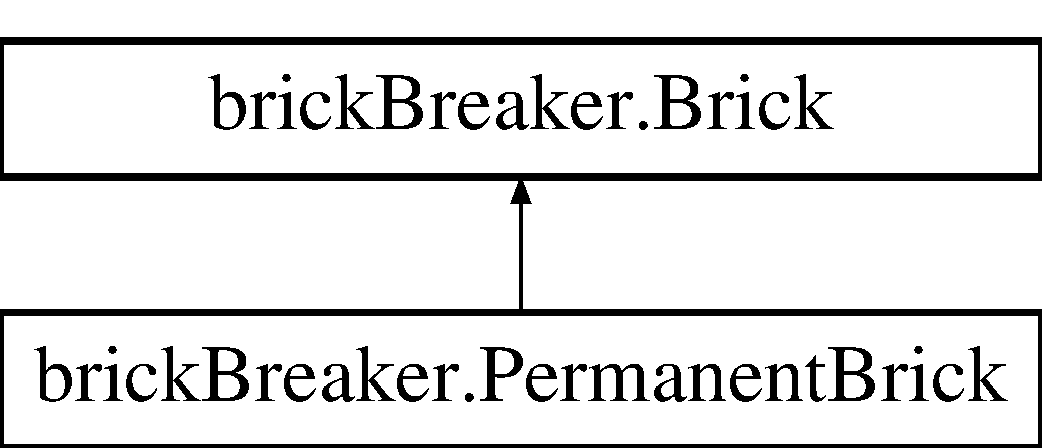
\includegraphics[height=2cm]{classbrick_breaker_1_1_permanent_brick}
\end{center}
\end{figure}
\subsection*{Public Member Functions}
\begin{DoxyCompactItemize}
\item 
\hyperlink{classbrick_breaker_1_1_permanent_brick_acb1d6072727e429556038041cfcf411a}{PermanentBrick} ()
\item 
boolean \hyperlink{classbrick_breaker_1_1_permanent_brick_a5095518bc2226f3257202d99e37d8ae4}{permanent} ()
\end{DoxyCompactItemize}


\subsection{Constructor \& Destructor Documentation}
\hypertarget{classbrick_breaker_1_1_permanent_brick_acb1d6072727e429556038041cfcf411a}{
\index{brickBreaker::PermanentBrick@{brickBreaker::PermanentBrick}!PermanentBrick@{PermanentBrick}}
\index{PermanentBrick@{PermanentBrick}!brickBreaker::PermanentBrick@{brickBreaker::PermanentBrick}}
\subsubsection[{PermanentBrick}]{\setlength{\rightskip}{0pt plus 5cm}brickBreaker.PermanentBrick.PermanentBrick ()}}
\label{classbrick_breaker_1_1_permanent_brick_acb1d6072727e429556038041cfcf411a}
Constructor 

\subsection{Member Function Documentation}
\hypertarget{classbrick_breaker_1_1_permanent_brick_a5095518bc2226f3257202d99e37d8ae4}{
\index{brickBreaker::PermanentBrick@{brickBreaker::PermanentBrick}!permanent@{permanent}}
\index{permanent@{permanent}!brickBreaker::PermanentBrick@{brickBreaker::PermanentBrick}}
\subsubsection[{permanent}]{\setlength{\rightskip}{0pt plus 5cm}boolean brickBreaker.PermanentBrick.permanent ()}}
\label{classbrick_breaker_1_1_permanent_brick_a5095518bc2226f3257202d99e37d8ae4}
Always returns true, since this brick is by definition permanent. 

Reimplemented from \hyperlink{classbrick_breaker_1_1_brick_a5fa03da94163b3dc3707c030e85a1405}{brickBreaker.Brick}.



The documentation for this class was generated from the following file:\begin{DoxyCompactItemize}
\item 
src/game/brickBreaker/\hyperlink{_permanent_brick_8java}{PermanentBrick.java}\end{DoxyCompactItemize}

\hypertarget{classbrick_breaker_1_1_power_brick}{
\section{brickBreaker.PowerBrick Class Reference}
\label{classbrick_breaker_1_1_power_brick}\index{brickBreaker::PowerBrick@{brickBreaker::PowerBrick}}
}
Inheritance diagram for brickBreaker.PowerBrick:\begin{figure}[H]
\begin{center}
\leavevmode
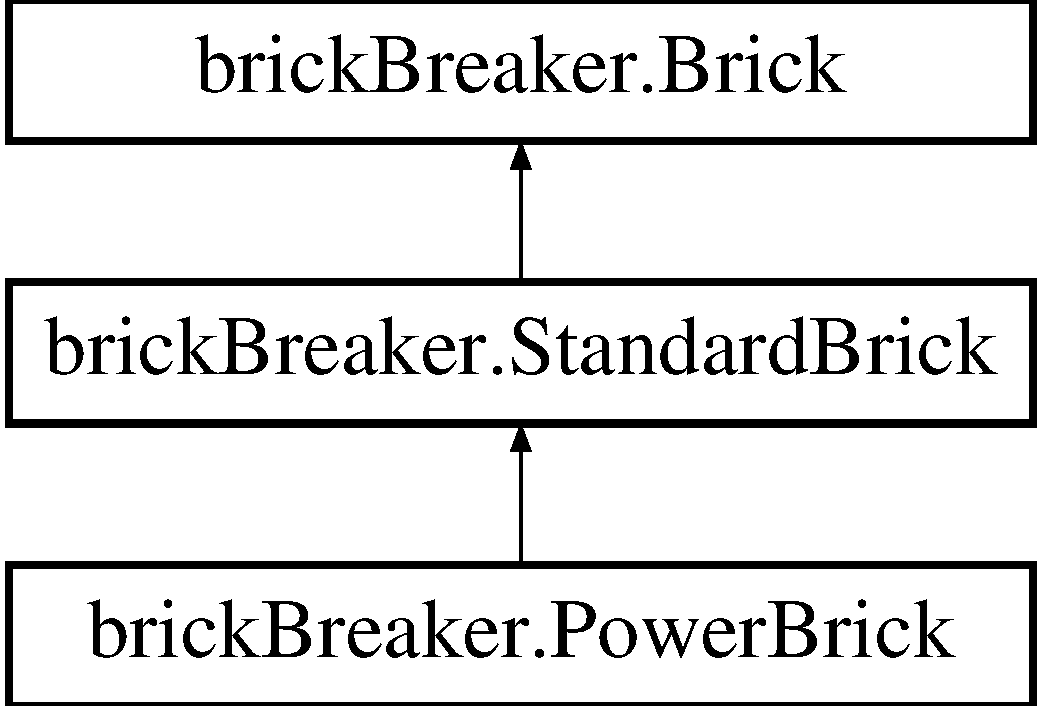
\includegraphics[height=3cm]{classbrick_breaker_1_1_power_brick}
\end{center}
\end{figure}
\subsection*{Public Member Functions}
\begin{DoxyCompactItemize}
\item 
\hyperlink{classbrick_breaker_1_1_power_brick_ab9512df794d4c4991067f9eb6c085399}{PowerBrick} ()
\item 
void \hyperlink{classbrick_breaker_1_1_power_brick_aa5f41bb48fc63ed441ec2e9892ccdac3}{powerUp} (\hyperlink{classbrick_breaker_1_1_ball}{Ball} b)
\end{DoxyCompactItemize}


\subsection{Constructor \& Destructor Documentation}
\hypertarget{classbrick_breaker_1_1_power_brick_ab9512df794d4c4991067f9eb6c085399}{
\index{brickBreaker::PowerBrick@{brickBreaker::PowerBrick}!PowerBrick@{PowerBrick}}
\index{PowerBrick@{PowerBrick}!brickBreaker::PowerBrick@{brickBreaker::PowerBrick}}
\subsubsection[{PowerBrick}]{\setlength{\rightskip}{0pt plus 5cm}brickBreaker.PowerBrick.PowerBrick ()}}
\label{classbrick_breaker_1_1_power_brick_ab9512df794d4c4991067f9eb6c085399}
Constructor 

\subsection{Member Function Documentation}
\hypertarget{classbrick_breaker_1_1_power_brick_aa5f41bb48fc63ed441ec2e9892ccdac3}{
\index{brickBreaker::PowerBrick@{brickBreaker::PowerBrick}!powerUp@{powerUp}}
\index{powerUp@{powerUp}!brickBreaker::PowerBrick@{brickBreaker::PowerBrick}}
\subsubsection[{powerUp}]{\setlength{\rightskip}{0pt plus 5cm}void brickBreaker.PowerBrick.powerUp ({\bf Ball} {\em b})}}
\label{classbrick_breaker_1_1_power_brick_aa5f41bb48fc63ed441ec2e9892ccdac3}
Increases the speed and point multiplier of the given ball. 
\begin{DoxyParams}{Parameters}
\item[{\em b}]The ball object to be updated \end{DoxyParams}


Reimplemented from \hyperlink{classbrick_breaker_1_1_brick_a109d6d8023e528284c1726ee55c3e50e}{brickBreaker.Brick}.



The documentation for this class was generated from the following file:\begin{DoxyCompactItemize}
\item 
game/brickBreaker/\hyperlink{_power_brick_8java}{PowerBrick.java}\end{DoxyCompactItemize}

\hypertarget{classbrick_breaker_1_1_p_r_panel}{
\section{brickBreaker.PRPanel Class Reference}
\label{classbrick_breaker_1_1_p_r_panel}\index{brickBreaker::PRPanel@{brickBreaker::PRPanel}}
}
Inheritance diagram for brickBreaker.PRPanel:\begin{figure}[H]
\begin{center}
\leavevmode
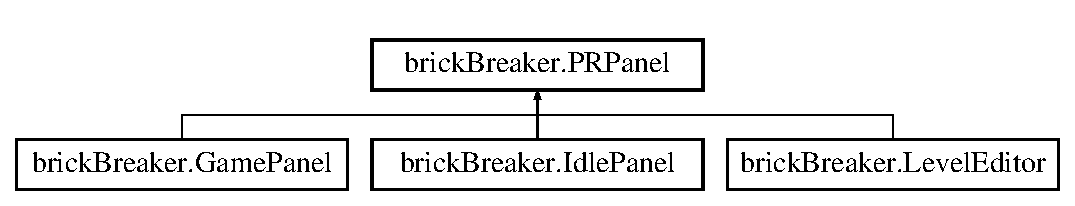
\includegraphics[height=2cm]{classbrick_breaker_1_1_p_r_panel}
\end{center}
\end{figure}
\subsection*{Public Member Functions}
\begin{DoxyCompactItemize}
\item 
void \hyperlink{classbrick_breaker_1_1_p_r_panel_a0868e501fc5599973492e6f0c53da920}{pause} ()
\item 
void \hyperlink{classbrick_breaker_1_1_p_r_panel_ac9aadc88543f9032a27f3eb2b8ea908b}{resume} ()
\item 
void \hyperlink{classbrick_breaker_1_1_p_r_panel_ad077fab978f84663f366a6fdde5efe6c}{stop} ()
\item 
void \hyperlink{classbrick_breaker_1_1_p_r_panel_a94e190e70d6aa937068cbf5e8cff523e}{start} ()
\item 
void \hyperlink{classbrick_breaker_1_1_p_r_panel_af86ccc2d42dc48eb03fb6db22e593fc2}{keyPressed} (KeyEvent e)
\item 
void \hyperlink{classbrick_breaker_1_1_p_r_panel_a3485136bec68dd500b98039bd7a87e8e}{keyReleased} (KeyEvent e)
\item 
void \hyperlink{classbrick_breaker_1_1_p_r_panel_a51bdf51ab7141c16101753e4180c970a}{keyTyped} (KeyEvent e)
\end{DoxyCompactItemize}


\subsection{Member Function Documentation}
\hypertarget{classbrick_breaker_1_1_p_r_panel_af86ccc2d42dc48eb03fb6db22e593fc2}{
\index{brickBreaker::PRPanel@{brickBreaker::PRPanel}!keyPressed@{keyPressed}}
\index{keyPressed@{keyPressed}!brickBreaker::PRPanel@{brickBreaker::PRPanel}}
\subsubsection[{keyPressed}]{\setlength{\rightskip}{0pt plus 5cm}void brickBreaker.PRPanel.keyPressed (KeyEvent {\em e})}}
\label{classbrick_breaker_1_1_p_r_panel_af86ccc2d42dc48eb03fb6db22e593fc2}
Inherited from KeyListener 

Reimplemented in \hyperlink{classbrick_breaker_1_1_game_panel_abf3d766d8fff87e69bfaf8ff59c438f3}{brickBreaker.GamePanel}.

\hypertarget{classbrick_breaker_1_1_p_r_panel_a3485136bec68dd500b98039bd7a87e8e}{
\index{brickBreaker::PRPanel@{brickBreaker::PRPanel}!keyReleased@{keyReleased}}
\index{keyReleased@{keyReleased}!brickBreaker::PRPanel@{brickBreaker::PRPanel}}
\subsubsection[{keyReleased}]{\setlength{\rightskip}{0pt plus 5cm}void brickBreaker.PRPanel.keyReleased (KeyEvent {\em e})}}
\label{classbrick_breaker_1_1_p_r_panel_a3485136bec68dd500b98039bd7a87e8e}
Inherited from KeyListener 

Reimplemented in \hyperlink{classbrick_breaker_1_1_game_panel_a8c41cc926e88dc8d1a1c241e6b9ef12e}{brickBreaker.GamePanel}.

\hypertarget{classbrick_breaker_1_1_p_r_panel_a51bdf51ab7141c16101753e4180c970a}{
\index{brickBreaker::PRPanel@{brickBreaker::PRPanel}!keyTyped@{keyTyped}}
\index{keyTyped@{keyTyped}!brickBreaker::PRPanel@{brickBreaker::PRPanel}}
\subsubsection[{keyTyped}]{\setlength{\rightskip}{0pt plus 5cm}void brickBreaker.PRPanel.keyTyped (KeyEvent {\em e})}}
\label{classbrick_breaker_1_1_p_r_panel_a51bdf51ab7141c16101753e4180c970a}
Inherited from KeyListener 

Reimplemented in \hyperlink{classbrick_breaker_1_1_game_panel_a23a455353c5904274a39f0f224cb0005}{brickBreaker.GamePanel}.

\hypertarget{classbrick_breaker_1_1_p_r_panel_a0868e501fc5599973492e6f0c53da920}{
\index{brickBreaker::PRPanel@{brickBreaker::PRPanel}!pause@{pause}}
\index{pause@{pause}!brickBreaker::PRPanel@{brickBreaker::PRPanel}}
\subsubsection[{pause}]{\setlength{\rightskip}{0pt plus 5cm}void brickBreaker.PRPanel.pause ()}}
\label{classbrick_breaker_1_1_p_r_panel_a0868e501fc5599973492e6f0c53da920}
Pause the panel's current action. 

Reimplemented in \hyperlink{classbrick_breaker_1_1_game_panel_a74382da15296d8ed9be081e4e6af72cc}{brickBreaker.GamePanel}, \hyperlink{classbrick_breaker_1_1_idle_panel_a42b96627662408932245a672b5fbfaf1}{brickBreaker.IdlePanel}, and \hyperlink{classbrick_breaker_1_1_level_editor_a5c1da01da393e14dbd38039bc457f713}{brickBreaker.LevelEditor}.

\hypertarget{classbrick_breaker_1_1_p_r_panel_ac9aadc88543f9032a27f3eb2b8ea908b}{
\index{brickBreaker::PRPanel@{brickBreaker::PRPanel}!resume@{resume}}
\index{resume@{resume}!brickBreaker::PRPanel@{brickBreaker::PRPanel}}
\subsubsection[{resume}]{\setlength{\rightskip}{0pt plus 5cm}void brickBreaker.PRPanel.resume ()}}
\label{classbrick_breaker_1_1_p_r_panel_ac9aadc88543f9032a27f3eb2b8ea908b}
Resume the panel's current action. 

Reimplemented in \hyperlink{classbrick_breaker_1_1_game_panel_af987d9ffe6d1d68941a93547bab41cfe}{brickBreaker.GamePanel}, \hyperlink{classbrick_breaker_1_1_idle_panel_ab04b565d2e626077051cefb27772a98f}{brickBreaker.IdlePanel}, and \hyperlink{classbrick_breaker_1_1_level_editor_a25e9ea0a6e91f1848c3b76f66a238789}{brickBreaker.LevelEditor}.

\hypertarget{classbrick_breaker_1_1_p_r_panel_a94e190e70d6aa937068cbf5e8cff523e}{
\index{brickBreaker::PRPanel@{brickBreaker::PRPanel}!start@{start}}
\index{start@{start}!brickBreaker::PRPanel@{brickBreaker::PRPanel}}
\subsubsection[{start}]{\setlength{\rightskip}{0pt plus 5cm}void brickBreaker.PRPanel.start ()}}
\label{classbrick_breaker_1_1_p_r_panel_a94e190e70d6aa937068cbf5e8cff523e}
Refresh the panel to it's starting state 

Reimplemented in \hyperlink{classbrick_breaker_1_1_game_panel_ac06637c2b612d44711aebefde82249bc}{brickBreaker.GamePanel}, \hyperlink{classbrick_breaker_1_1_idle_panel_ad391091a78283ca2546e52f967d46ed6}{brickBreaker.IdlePanel}, and \hyperlink{classbrick_breaker_1_1_level_editor_ab2df7eb7b75f4e87b25c4b2d9422dc3d}{brickBreaker.LevelEditor}.

\hypertarget{classbrick_breaker_1_1_p_r_panel_ad077fab978f84663f366a6fdde5efe6c}{
\index{brickBreaker::PRPanel@{brickBreaker::PRPanel}!stop@{stop}}
\index{stop@{stop}!brickBreaker::PRPanel@{brickBreaker::PRPanel}}
\subsubsection[{stop}]{\setlength{\rightskip}{0pt plus 5cm}void brickBreaker.PRPanel.stop ()}}
\label{classbrick_breaker_1_1_p_r_panel_ad077fab978f84663f366a6fdde5efe6c}
Stop the panel's action completely. 

Reimplemented in \hyperlink{classbrick_breaker_1_1_game_panel_adda952b668cd479832134a4c0ddfbc41}{brickBreaker.GamePanel}, \hyperlink{classbrick_breaker_1_1_idle_panel_a2334ae977477929eeb82dbba53384360}{brickBreaker.IdlePanel}, and \hyperlink{classbrick_breaker_1_1_level_editor_aa38941ac69b2b38f472fd402d3e33e40}{brickBreaker.LevelEditor}.



The documentation for this class was generated from the following file:\begin{DoxyCompactItemize}
\item 
src/game/brickBreaker/\hyperlink{_p_r_panel_8java}{PRPanel.java}\end{DoxyCompactItemize}

\hypertarget{classbrick_breaker_1_1_racket}{
\section{brickBreaker.Racket Class Reference}
\label{classbrick_breaker_1_1_racket}\index{brickBreaker::Racket@{brickBreaker::Racket}}
}
Inheritance diagram for brickBreaker.Racket:\begin{figure}[H]
\begin{center}
\leavevmode
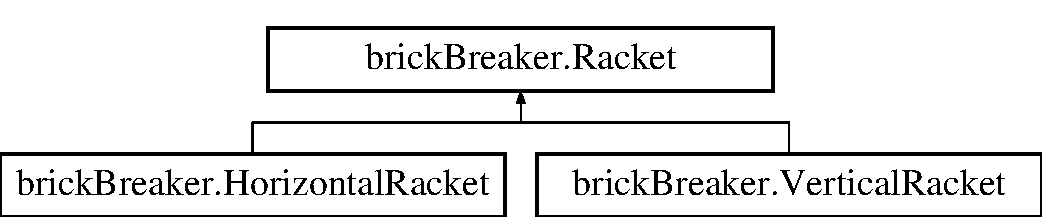
\includegraphics[height=2cm]{classbrick_breaker_1_1_racket}
\end{center}
\end{figure}
\subsection*{Public Member Functions}
\begin{DoxyCompactItemize}
\item 
\hypertarget{classbrick_breaker_1_1_racket_a350fa11540f07d2eed108a1aa75240e2}{
void {\bfseries setMovingLeft} ()}
\label{classbrick_breaker_1_1_racket_a350fa11540f07d2eed108a1aa75240e2}

\item 
\hypertarget{classbrick_breaker_1_1_racket_ac2bdea9a9f15d06648f2c2094ff123ba}{
void {\bfseries setMovingRight} ()}
\label{classbrick_breaker_1_1_racket_ac2bdea9a9f15d06648f2c2094ff123ba}

\item 
\hypertarget{classbrick_breaker_1_1_racket_a1d5ee505bd935fa6b8ea6001c15a57b9}{
void {\bfseries stop} ()}
\label{classbrick_breaker_1_1_racket_a1d5ee505bd935fa6b8ea6001c15a57b9}

\item 
\hypertarget{classbrick_breaker_1_1_racket_ab439c6379d04064940f4a09007d5fe4c}{
void {\bfseries updatePos} ()}
\label{classbrick_breaker_1_1_racket_ab439c6379d04064940f4a09007d5fe4c}

\item 
\hypertarget{classbrick_breaker_1_1_racket_ab92ecb01070ce2fdefd99c3cc5212994}{
void {\bfseries moveLeft} ()}
\label{classbrick_breaker_1_1_racket_ab92ecb01070ce2fdefd99c3cc5212994}

\item 
\hypertarget{classbrick_breaker_1_1_racket_a755ac54ffa2ff2013442cda726fcf268}{
void {\bfseries moveRight} ()}
\label{classbrick_breaker_1_1_racket_a755ac54ffa2ff2013442cda726fcf268}

\item 
\hypertarget{classbrick_breaker_1_1_racket_a8d29bc2897ed97686e2be3e96308629b}{
int {\bfseries getLeft} ()}
\label{classbrick_breaker_1_1_racket_a8d29bc2897ed97686e2be3e96308629b}

\item 
\hypertarget{classbrick_breaker_1_1_racket_ad947f4853fbe782ab81e5a90e87ec360}{
int {\bfseries getRight} ()}
\label{classbrick_breaker_1_1_racket_ad947f4853fbe782ab81e5a90e87ec360}

\item 
\hypertarget{classbrick_breaker_1_1_racket_ac70c03dfe6eff9485e79e1430a0a2ab0}{
int {\bfseries getX} ()}
\label{classbrick_breaker_1_1_racket_ac70c03dfe6eff9485e79e1430a0a2ab0}

\item 
\hypertarget{classbrick_breaker_1_1_racket_a229e48b5cacbc3921f8c626b77489e9b}{
int {\bfseries getY} ()}
\label{classbrick_breaker_1_1_racket_a229e48b5cacbc3921f8c626b77489e9b}

\item 
\hypertarget{classbrick_breaker_1_1_racket_a32acec6ccc8fd726507697371bcde2c0}{
int {\bfseries getWidth} ()}
\label{classbrick_breaker_1_1_racket_a32acec6ccc8fd726507697371bcde2c0}

\item 
\hypertarget{classbrick_breaker_1_1_racket_a6ca0308def67e0955522a0e0beb430e9}{
abstract void {\bfseries draw} (Graphics g)}
\label{classbrick_breaker_1_1_racket_a6ca0308def67e0955522a0e0beb430e9}

\item 
\hypertarget{classbrick_breaker_1_1_racket_a81880bdbdfda6ec88d1d4e7fc72f8f74}{
abstract \hyperlink{classbrick_breaker_1_1_ball}{Ball} {\bfseries checkCollision} (\hyperlink{classbrick_breaker_1_1_ball}{Ball} ball)}
\label{classbrick_breaker_1_1_racket_a81880bdbdfda6ec88d1d4e7fc72f8f74}

\item 
\hypertarget{classbrick_breaker_1_1_racket_a129dbc802cd26299ebca916283edbe27}{
abstract boolean {\bfseries checkPast} (\hyperlink{classbrick_breaker_1_1_ball}{Ball} ball)}
\label{classbrick_breaker_1_1_racket_a129dbc802cd26299ebca916283edbe27}

\item 
\hypertarget{classbrick_breaker_1_1_racket_af8ef3d348dca4cc1daad627826baea56}{
boolean {\bfseries isLeft} ()}
\label{classbrick_breaker_1_1_racket_af8ef3d348dca4cc1daad627826baea56}

\item 
\hypertarget{classbrick_breaker_1_1_racket_ad1d76aea1bd7dea3c4114c8c585150ed}{
boolean {\bfseries isRight} ()}
\label{classbrick_breaker_1_1_racket_ad1d76aea1bd7dea3c4114c8c585150ed}

\item 
\hypertarget{classbrick_breaker_1_1_racket_a0bd80cbd11ffe9afd6212e2d96a88554}{
boolean {\bfseries isTop} ()}
\label{classbrick_breaker_1_1_racket_a0bd80cbd11ffe9afd6212e2d96a88554}

\item 
\hypertarget{classbrick_breaker_1_1_racket_a908f0a42e73739db9fd0734d6a4fdb2f}{
boolean {\bfseries isBottom} ()}
\label{classbrick_breaker_1_1_racket_a908f0a42e73739db9fd0734d6a4fdb2f}

\end{DoxyCompactItemize}
\subsection*{Static Public Attributes}
\begin{DoxyCompactItemize}
\item 
\hypertarget{classbrick_breaker_1_1_racket_a08c1b8b4b30224b78b854b11cfbb6710}{
static final double {\bfseries maxSpeed} = 8.0}
\label{classbrick_breaker_1_1_racket_a08c1b8b4b30224b78b854b11cfbb6710}

\item 
\hypertarget{classbrick_breaker_1_1_racket_aed61315731a5be300989a390f009abd8}{
static int {\bfseries thickness} = 5}
\label{classbrick_breaker_1_1_racket_aed61315731a5be300989a390f009abd8}

\end{DoxyCompactItemize}
\subsection*{Protected Attributes}
\begin{DoxyCompactItemize}
\item 
\hypertarget{classbrick_breaker_1_1_racket_a14604c7182eb6f3ed8285a0b88fbf26f}{
int {\bfseries range}}
\label{classbrick_breaker_1_1_racket_a14604c7182eb6f3ed8285a0b88fbf26f}

\item 
\hypertarget{classbrick_breaker_1_1_racket_abb3c0be790adfb946af95d700e9498e3}{
int {\bfseries width}}
\label{classbrick_breaker_1_1_racket_abb3c0be790adfb946af95d700e9498e3}

\item 
\hypertarget{classbrick_breaker_1_1_racket_aa9e386519155ef9bc1675f04c25dfc11}{
double {\bfseries posX}}
\label{classbrick_breaker_1_1_racket_aa9e386519155ef9bc1675f04c25dfc11}

\item 
\hypertarget{classbrick_breaker_1_1_racket_a087c2386f299c432c5ad4c6c6c274f81}{
double {\bfseries posY}}
\label{classbrick_breaker_1_1_racket_a087c2386f299c432c5ad4c6c6c274f81}

\item 
\hypertarget{classbrick_breaker_1_1_racket_ab8a7a0111d64fe89d58b2f375d701047}{
double {\bfseries speed} = 0}
\label{classbrick_breaker_1_1_racket_ab8a7a0111d64fe89d58b2f375d701047}

\item 
\hypertarget{classbrick_breaker_1_1_racket_a5fcccad4ce0ba0cfa26ae2cf1501a601}{
Color {\bfseries color} = Color.blue}
\label{classbrick_breaker_1_1_racket_a5fcccad4ce0ba0cfa26ae2cf1501a601}

\item 
\hypertarget{classbrick_breaker_1_1_racket_a0749ef4c81abf63c8ee1d012ffd90155}{
boolean {\bfseries movingRight}}
\label{classbrick_breaker_1_1_racket_a0749ef4c81abf63c8ee1d012ffd90155}

\item 
\hypertarget{classbrick_breaker_1_1_racket_a88667ee5bc44b240cac5817ffb088a52}{
boolean {\bfseries movingLeft}}
\label{classbrick_breaker_1_1_racket_a88667ee5bc44b240cac5817ffb088a52}

\end{DoxyCompactItemize}


\subsection{Detailed Description}
Abstract class \hyperlink{classbrick_breaker_1_1_racket}{Racket} -\/ write a description of the class here

\begin{DoxyAuthor}{Author}
(your name here) 
\end{DoxyAuthor}
\begin{DoxyVersion}{Version}
(version number or date here) 
\end{DoxyVersion}


The documentation for this class was generated from the following file:\begin{DoxyCompactItemize}
\item 
game/brickBreaker/Racket.java\end{DoxyCompactItemize}

\hypertarget{classbrick_breaker_1_1web_1_1_request_failure_exception}{
\section{brickBreaker.web.RequestFailureException Class Reference}
\label{classbrick_breaker_1_1web_1_1_request_failure_exception}\index{brickBreaker::web::RequestFailureException@{brickBreaker::web::RequestFailureException}}
}
\subsection*{Public Member Functions}
\begin{DoxyCompactItemize}
\item 
\hyperlink{classbrick_breaker_1_1web_1_1_request_failure_exception_aabe6d2ef76adb37a25d7d828be02fb3f}{RequestFailureException} ()
\item 
\hyperlink{classbrick_breaker_1_1web_1_1_request_failure_exception_ac88ada25c67073741864d896fc6192a7}{RequestFailureException} (String message)
\item 
\hyperlink{classbrick_breaker_1_1web_1_1_request_failure_exception_ab61c4dda3a1de78730729cd4b42d6863}{RequestFailureException} (String message, Throwable cause)
\item 
\hyperlink{classbrick_breaker_1_1web_1_1_request_failure_exception_ab1b4d46e0cfbbe6a3402d6f1d733bd82}{RequestFailureException} (Throwable cause)
\end{DoxyCompactItemize}


\subsection{Detailed Description}
This class provides an application-\/specific wrapper for exceptions caused by a failure to complete a request to a remote server.

\begin{DoxyAuthor}{Author}
Abraham Lin 
\end{DoxyAuthor}


\subsection{Constructor \& Destructor Documentation}
\hypertarget{classbrick_breaker_1_1web_1_1_request_failure_exception_aabe6d2ef76adb37a25d7d828be02fb3f}{
\index{brickBreaker::web::RequestFailureException@{brickBreaker::web::RequestFailureException}!RequestFailureException@{RequestFailureException}}
\index{RequestFailureException@{RequestFailureException}!brickBreaker::web::RequestFailureException@{brickBreaker::web::RequestFailureException}}
\subsubsection[{RequestFailureException}]{\setlength{\rightskip}{0pt plus 5cm}brickBreaker.web.RequestFailureException.RequestFailureException ()}}
\label{classbrick_breaker_1_1web_1_1_request_failure_exception_aabe6d2ef76adb37a25d7d828be02fb3f}
Constructs a new {\ttfamily \hyperlink{classbrick_breaker_1_1web_1_1_request_failure_exception}{RequestFailureException}} with {\ttfamily null} as its detail message. \hypertarget{classbrick_breaker_1_1web_1_1_request_failure_exception_ac88ada25c67073741864d896fc6192a7}{
\index{brickBreaker::web::RequestFailureException@{brickBreaker::web::RequestFailureException}!RequestFailureException@{RequestFailureException}}
\index{RequestFailureException@{RequestFailureException}!brickBreaker::web::RequestFailureException@{brickBreaker::web::RequestFailureException}}
\subsubsection[{RequestFailureException}]{\setlength{\rightskip}{0pt plus 5cm}brickBreaker.web.RequestFailureException.RequestFailureException (String {\em message})}}
\label{classbrick_breaker_1_1web_1_1_request_failure_exception_ac88ada25c67073741864d896fc6192a7}
Constructs a new {\ttfamily \hyperlink{classbrick_breaker_1_1web_1_1_request_failure_exception}{RequestFailureException}} with the specified detail message.


\begin{DoxyParams}{Parameters}
\item[{\em message}]the detail message \end{DoxyParams}
\hypertarget{classbrick_breaker_1_1web_1_1_request_failure_exception_ab61c4dda3a1de78730729cd4b42d6863}{
\index{brickBreaker::web::RequestFailureException@{brickBreaker::web::RequestFailureException}!RequestFailureException@{RequestFailureException}}
\index{RequestFailureException@{RequestFailureException}!brickBreaker::web::RequestFailureException@{brickBreaker::web::RequestFailureException}}
\subsubsection[{RequestFailureException}]{\setlength{\rightskip}{0pt plus 5cm}brickBreaker.web.RequestFailureException.RequestFailureException (String {\em message}, \/  Throwable {\em cause})}}
\label{classbrick_breaker_1_1web_1_1_request_failure_exception_ab61c4dda3a1de78730729cd4b42d6863}
Constructs a new {\ttfamily \hyperlink{classbrick_breaker_1_1web_1_1_request_failure_exception}{RequestFailureException}} with the specified detail message and cause.


\begin{DoxyParams}{Parameters}
\item[{\em message}]the detail message \item[{\em cause}]the cause \end{DoxyParams}
\hypertarget{classbrick_breaker_1_1web_1_1_request_failure_exception_ab1b4d46e0cfbbe6a3402d6f1d733bd82}{
\index{brickBreaker::web::RequestFailureException@{brickBreaker::web::RequestFailureException}!RequestFailureException@{RequestFailureException}}
\index{RequestFailureException@{RequestFailureException}!brickBreaker::web::RequestFailureException@{brickBreaker::web::RequestFailureException}}
\subsubsection[{RequestFailureException}]{\setlength{\rightskip}{0pt plus 5cm}brickBreaker.web.RequestFailureException.RequestFailureException (Throwable {\em cause})}}
\label{classbrick_breaker_1_1web_1_1_request_failure_exception_ab1b4d46e0cfbbe6a3402d6f1d733bd82}
Constructs a new {\ttfamily \hyperlink{classbrick_breaker_1_1web_1_1_request_failure_exception}{RequestFailureException}} with the specified cause.


\begin{DoxyParams}{Parameters}
\item[{\em cause}]the cause \end{DoxyParams}


The documentation for this class was generated from the following file:\begin{DoxyCompactItemize}
\item 
game/brickBreaker/web/RequestFailureException.java\end{DoxyCompactItemize}

\hypertarget{classbrick_breaker_1_1_standard_brick}{
\section{brickBreaker.StandardBrick Class Reference}
\label{classbrick_breaker_1_1_standard_brick}\index{brickBreaker::StandardBrick@{brickBreaker::StandardBrick}}
}
Inheritance diagram for brickBreaker.StandardBrick:\begin{figure}[H]
\begin{center}
\leavevmode
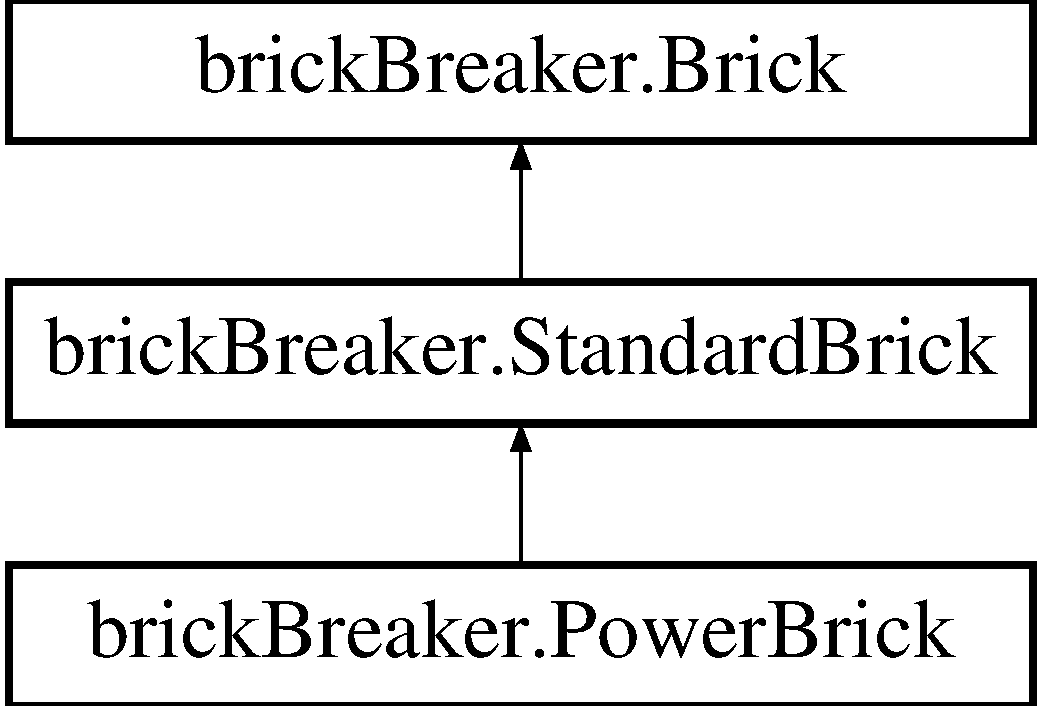
\includegraphics[height=3cm]{classbrick_breaker_1_1_standard_brick}
\end{center}
\end{figure}
\subsection*{Public Member Functions}
\begin{DoxyCompactItemize}
\item 
\hyperlink{classbrick_breaker_1_1_standard_brick_a5521bf7ca0eeea9c887995f644654b46}{StandardBrick} ()
\item 
\hyperlink{classbrick_breaker_1_1_standard_brick_a035ddbcb9121dfa674c87518ae0d710e}{StandardBrick} (int pts, int hits, Color c)
\end{DoxyCompactItemize}


\subsection{Constructor \& Destructor Documentation}
\hypertarget{classbrick_breaker_1_1_standard_brick_a5521bf7ca0eeea9c887995f644654b46}{
\index{brickBreaker::StandardBrick@{brickBreaker::StandardBrick}!StandardBrick@{StandardBrick}}
\index{StandardBrick@{StandardBrick}!brickBreaker::StandardBrick@{brickBreaker::StandardBrick}}
\subsubsection[{StandardBrick}]{\setlength{\rightskip}{0pt plus 5cm}brickBreaker.StandardBrick.StandardBrick ()}}
\label{classbrick_breaker_1_1_standard_brick_a5521bf7ca0eeea9c887995f644654b46}
Default constructor \hypertarget{classbrick_breaker_1_1_standard_brick_a035ddbcb9121dfa674c87518ae0d710e}{
\index{brickBreaker::StandardBrick@{brickBreaker::StandardBrick}!StandardBrick@{StandardBrick}}
\index{StandardBrick@{StandardBrick}!brickBreaker::StandardBrick@{brickBreaker::StandardBrick}}
\subsubsection[{StandardBrick}]{\setlength{\rightskip}{0pt plus 5cm}brickBreaker.StandardBrick.StandardBrick (int {\em pts}, \/  int {\em hits}, \/  Color {\em c})}}
\label{classbrick_breaker_1_1_standard_brick_a035ddbcb9121dfa674c87518ae0d710e}
Constructor


\begin{DoxyParams}{Parameters}
\item[{\em pts}]Points earned when the brick is removed \item[{\em hits}]Number of hits to remove the brick \item[{\em c}]\hyperlink{classbrick_breaker_1_1_brick}{Brick} color \end{DoxyParams}


The documentation for this class was generated from the following file:\begin{DoxyCompactItemize}
\item 
src/game/brickBreaker/\hyperlink{_standard_brick_8java}{StandardBrick.java}\end{DoxyCompactItemize}

\hypertarget{classbrick_breaker_1_1_start}{
\section{brickBreaker.Start Class Reference}
\label{classbrick_breaker_1_1_start}\index{brickBreaker::Start@{brickBreaker::Start}}
}
\subsection*{Public Member Functions}
\begin{DoxyCompactItemize}
\item 
\hypertarget{classbrick_breaker_1_1_start_add9cb12f31b41a4c48a9631e3b813bfc}{
{\bfseries Start} (boolean loggedIn)}
\label{classbrick_breaker_1_1_start_add9cb12f31b41a4c48a9631e3b813bfc}

\item 
\hypertarget{classbrick_breaker_1_1_start_afe4437abe9e58312599f173ef8cc3033}{
void {\bfseries startGame} (\hyperlink{classbrick_breaker_1_1_level}{Level} lev)}
\label{classbrick_breaker_1_1_start_afe4437abe9e58312599f173ef8cc3033}

\item 
\hypertarget{classbrick_breaker_1_1_start_a794a63dad7a962820d9dd5bf26bf2e35}{
void {\bfseries endGame} (\hyperlink{classbrick_breaker_1_1_level}{Level} lev, int score)}
\label{classbrick_breaker_1_1_start_a794a63dad7a962820d9dd5bf26bf2e35}

\item 
\hypertarget{classbrick_breaker_1_1_start_a398e72365f82fe4214ea3534bfa34270}{
void {\bfseries startEditor} ()}
\label{classbrick_breaker_1_1_start_a398e72365f82fe4214ea3534bfa34270}

\item 
\hypertarget{classbrick_breaker_1_1_start_af99a0afe969ad087b6315a19e8b2289c}{
void {\bfseries exitEditor} ()}
\label{classbrick_breaker_1_1_start_af99a0afe969ad087b6315a19e8b2289c}

\item 
\hypertarget{classbrick_breaker_1_1_start_a8a00f5a3b3b443b9d54ea98808ffab37}{
void {\bfseries windowActivated} (WindowEvent e)}
\label{classbrick_breaker_1_1_start_a8a00f5a3b3b443b9d54ea98808ffab37}

\item 
\hypertarget{classbrick_breaker_1_1_start_ac2c1907f281e5cc6abf558789c8946b3}{
void {\bfseries windowDeactivated} (WindowEvent e)}
\label{classbrick_breaker_1_1_start_ac2c1907f281e5cc6abf558789c8946b3}

\item 
\hypertarget{classbrick_breaker_1_1_start_a7a77b64bcea5b507ae49463baa3f0282}{
void {\bfseries windowDeiconified} (WindowEvent e)}
\label{classbrick_breaker_1_1_start_a7a77b64bcea5b507ae49463baa3f0282}

\item 
\hypertarget{classbrick_breaker_1_1_start_aaadc30e22fd645a756381bedd0c35c9e}{
void {\bfseries windowIconified} (WindowEvent e)}
\label{classbrick_breaker_1_1_start_aaadc30e22fd645a756381bedd0c35c9e}

\item 
\hypertarget{classbrick_breaker_1_1_start_a11168f9afbcfc8cac2b7570a3a0dfa09}{
void {\bfseries windowClosing} (WindowEvent e)}
\label{classbrick_breaker_1_1_start_a11168f9afbcfc8cac2b7570a3a0dfa09}

\item 
\hypertarget{classbrick_breaker_1_1_start_a00d57f66b787a7eea85773c2f5c9fd62}{
void {\bfseries windowClosed} (WindowEvent e)}
\label{classbrick_breaker_1_1_start_a00d57f66b787a7eea85773c2f5c9fd62}

\item 
\hypertarget{classbrick_breaker_1_1_start_a0c42ef06bf5158b92edc91d34ee5c038}{
void {\bfseries windowOpened} (WindowEvent e)}
\label{classbrick_breaker_1_1_start_a0c42ef06bf5158b92edc91d34ee5c038}

\item 
\hypertarget{classbrick_breaker_1_1_start_a988d6bb03340ad92e27da5a3b6bef95d}{
void {\bfseries edit} ()}
\label{classbrick_breaker_1_1_start_a988d6bb03340ad92e27da5a3b6bef95d}

\end{DoxyCompactItemize}
\subsection*{Static Public Member Functions}
\begin{DoxyCompactItemize}
\item 
\hypertarget{classbrick_breaker_1_1_start_a1c5523121a86c315e8487d3dc826500c}{
static void {\bfseries main} (String args\mbox{[}$\,$\mbox{]})}
\label{classbrick_breaker_1_1_start_a1c5523121a86c315e8487d3dc826500c}

\end{DoxyCompactItemize}
\subsection*{Static Public Attributes}
\begin{DoxyCompactItemize}
\item 
\hypertarget{classbrick_breaker_1_1_start_a0cb22b25bc82b86148838e67d553453a}{
static int {\bfseries WIDTH} = 1000}
\label{classbrick_breaker_1_1_start_a0cb22b25bc82b86148838e67d553453a}

\item 
\hypertarget{classbrick_breaker_1_1_start_a06e396be377a68ab41caabfe45ba0951}{
static int {\bfseries HEIGHT} = 700}
\label{classbrick_breaker_1_1_start_a06e396be377a68ab41caabfe45ba0951}

\end{DoxyCompactItemize}
\subsection*{Package Attributes}
\begin{DoxyCompactItemize}
\item 
\hypertarget{classbrick_breaker_1_1_start_aa694e353f91972cfe69ffb36d09cdab9}{
Container {\bfseries c} = getContentPane()}
\label{classbrick_breaker_1_1_start_aa694e353f91972cfe69ffb36d09cdab9}

\end{DoxyCompactItemize}


The documentation for this class was generated from the following file:\begin{DoxyCompactItemize}
\item 
game/brickBreaker/Start.java\end{DoxyCompactItemize}

\hypertarget{classbrick_breaker_1_1_start_editor}{
\section{brickBreaker.StartEditor Class Reference}
\label{classbrick_breaker_1_1_start_editor}\index{brickBreaker::StartEditor@{brickBreaker::StartEditor}}
}
\subsection*{Static Public Member Functions}
\begin{DoxyCompactItemize}
\item 
static void \hyperlink{classbrick_breaker_1_1_start_editor_a2e6924e9e8162a7b1976ce5d01478bee}{main} (String args\mbox{[}$\,$\mbox{]})
\end{DoxyCompactItemize}


\subsection{Member Function Documentation}
\hypertarget{classbrick_breaker_1_1_start_editor_a2e6924e9e8162a7b1976ce5d01478bee}{
\index{brickBreaker::StartEditor@{brickBreaker::StartEditor}!main@{main}}
\index{main@{main}!brickBreaker::StartEditor@{brickBreaker::StartEditor}}
\subsubsection[{main}]{\setlength{\rightskip}{0pt plus 5cm}static void brickBreaker.StartEditor.main (String {\em args}\mbox{[}$\,$\mbox{]})\hspace{0.3cm}{\ttfamily  \mbox{[}static\mbox{]}}}}
\label{classbrick_breaker_1_1_start_editor_a2e6924e9e8162a7b1976ce5d01478bee}

\begin{DoxyParams}{Parameters}
\item[{\em args}]the command line arguments \end{DoxyParams}


The documentation for this class was generated from the following file:\begin{DoxyCompactItemize}
\item 
game/brickBreaker/StartEditor.java\end{DoxyCompactItemize}

\hypertarget{classbrick_breaker_1_1_start_idle}{
\section{brickBreaker.StartIdle Class Reference}
\label{classbrick_breaker_1_1_start_idle}\index{brickBreaker::StartIdle@{brickBreaker::StartIdle}}
}
\subsection*{Static Public Member Functions}
\begin{DoxyCompactItemize}
\item 
static void \hyperlink{classbrick_breaker_1_1_start_idle_a19cd517d36d1ee07d9bf3c6a8f10e018}{main} (String args\mbox{[}$\,$\mbox{]})
\end{DoxyCompactItemize}


\subsection{Detailed Description}
\begin{DoxyAuthor}{Author}
robert 
\end{DoxyAuthor}


\subsection{Member Function Documentation}
\hypertarget{classbrick_breaker_1_1_start_idle_a19cd517d36d1ee07d9bf3c6a8f10e018}{
\index{brickBreaker::StartIdle@{brickBreaker::StartIdle}!main@{main}}
\index{main@{main}!brickBreaker::StartIdle@{brickBreaker::StartIdle}}
\subsubsection[{main}]{\setlength{\rightskip}{0pt plus 5cm}static void brickBreaker.StartIdle.main (String {\em args}\mbox{[}$\,$\mbox{]})\hspace{0.3cm}{\ttfamily  \mbox{[}static\mbox{]}}}}
\label{classbrick_breaker_1_1_start_idle_a19cd517d36d1ee07d9bf3c6a8f10e018}

\begin{DoxyParams}{Parameters}
\item[{\em args}]the command line arguments \end{DoxyParams}


The documentation for this class was generated from the following file:\begin{DoxyCompactItemize}
\item 
src/game/brickBreaker/StartIdle.java\end{DoxyCompactItemize}

\hypertarget{classbrick_breaker_1_1web_1_1_user_config}{
\section{brickBreaker.web.UserConfig Class Reference}
\label{classbrick_breaker_1_1web_1_1_user_config}\index{brickBreaker::web::UserConfig@{brickBreaker::web::UserConfig}}
}
\subsection*{Public Member Functions}
\begin{DoxyCompactItemize}
\item 
String \hyperlink{classbrick_breaker_1_1web_1_1_user_config_a058016814e1d4b5b15c1708ed96e5acf}{getUsername} ()
\item 
void \hyperlink{classbrick_breaker_1_1web_1_1_user_config_a4565256db7d0f30cb7f4b63bd06a7472}{setUsername} (String username)
\item 
String \hyperlink{classbrick_breaker_1_1web_1_1_user_config_a06f536ee2fc04b8d49d42d0e110ff1dc}{getPassword} ()
\item 
void \hyperlink{classbrick_breaker_1_1web_1_1_user_config_a4b7cbc1a5c2e83db4e21ecc870b272c7}{setPassword} (String password)
\end{DoxyCompactItemize}
\subsection*{Static Public Member Functions}
\begin{DoxyCompactItemize}
\item 
static \hyperlink{classbrick_breaker_1_1web_1_1_user_config}{UserConfig} \hyperlink{classbrick_breaker_1_1web_1_1_user_config_a1d3a26745df81ea9335d7c1945400445}{getInstance} ()
\end{DoxyCompactItemize}


\subsection{Detailed Description}
This singleton class provides a centralized means of storing user credentials.

\begin{DoxyAuthor}{Author}
Abraham Lin 
\end{DoxyAuthor}


\subsection{Member Function Documentation}
\hypertarget{classbrick_breaker_1_1web_1_1_user_config_a1d3a26745df81ea9335d7c1945400445}{
\index{brickBreaker::web::UserConfig@{brickBreaker::web::UserConfig}!getInstance@{getInstance}}
\index{getInstance@{getInstance}!brickBreaker::web::UserConfig@{brickBreaker::web::UserConfig}}
\subsubsection[{getInstance}]{\setlength{\rightskip}{0pt plus 5cm}static {\bf UserConfig} brickBreaker.web.UserConfig.getInstance ()\hspace{0.3cm}{\ttfamily  \mbox{[}static\mbox{]}}}}
\label{classbrick_breaker_1_1web_1_1_user_config_a1d3a26745df81ea9335d7c1945400445}
Returns this {\ttfamily \hyperlink{classbrick_breaker_1_1web_1_1_user_config}{UserConfig}}.

\begin{DoxyReturn}{Returns}
this {\ttfamily \hyperlink{classbrick_breaker_1_1web_1_1_user_config}{UserConfig}} 
\end{DoxyReturn}
\hypertarget{classbrick_breaker_1_1web_1_1_user_config_a06f536ee2fc04b8d49d42d0e110ff1dc}{
\index{brickBreaker::web::UserConfig@{brickBreaker::web::UserConfig}!getPassword@{getPassword}}
\index{getPassword@{getPassword}!brickBreaker::web::UserConfig@{brickBreaker::web::UserConfig}}
\subsubsection[{getPassword}]{\setlength{\rightskip}{0pt plus 5cm}String brickBreaker.web.UserConfig.getPassword ()}}
\label{classbrick_breaker_1_1web_1_1_user_config_a06f536ee2fc04b8d49d42d0e110ff1dc}
Returns the current user's password.

\begin{DoxyReturn}{Returns}
the current user's password 
\end{DoxyReturn}
\hypertarget{classbrick_breaker_1_1web_1_1_user_config_a058016814e1d4b5b15c1708ed96e5acf}{
\index{brickBreaker::web::UserConfig@{brickBreaker::web::UserConfig}!getUsername@{getUsername}}
\index{getUsername@{getUsername}!brickBreaker::web::UserConfig@{brickBreaker::web::UserConfig}}
\subsubsection[{getUsername}]{\setlength{\rightskip}{0pt plus 5cm}String brickBreaker.web.UserConfig.getUsername ()}}
\label{classbrick_breaker_1_1web_1_1_user_config_a058016814e1d4b5b15c1708ed96e5acf}
Returns the current user's username.

\begin{DoxyReturn}{Returns}
the current user's username 
\end{DoxyReturn}
\hypertarget{classbrick_breaker_1_1web_1_1_user_config_a4b7cbc1a5c2e83db4e21ecc870b272c7}{
\index{brickBreaker::web::UserConfig@{brickBreaker::web::UserConfig}!setPassword@{setPassword}}
\index{setPassword@{setPassword}!brickBreaker::web::UserConfig@{brickBreaker::web::UserConfig}}
\subsubsection[{setPassword}]{\setlength{\rightskip}{0pt plus 5cm}void brickBreaker.web.UserConfig.setPassword (String {\em password})}}
\label{classbrick_breaker_1_1web_1_1_user_config_a4b7cbc1a5c2e83db4e21ecc870b272c7}
Sets the current user's password.


\begin{DoxyParams}{Parameters}
\item[{\em password}]the new password \end{DoxyParams}
\hypertarget{classbrick_breaker_1_1web_1_1_user_config_a4565256db7d0f30cb7f4b63bd06a7472}{
\index{brickBreaker::web::UserConfig@{brickBreaker::web::UserConfig}!setUsername@{setUsername}}
\index{setUsername@{setUsername}!brickBreaker::web::UserConfig@{brickBreaker::web::UserConfig}}
\subsubsection[{setUsername}]{\setlength{\rightskip}{0pt plus 5cm}void brickBreaker.web.UserConfig.setUsername (String {\em username})}}
\label{classbrick_breaker_1_1web_1_1_user_config_a4565256db7d0f30cb7f4b63bd06a7472}
Sets the current user's username.


\begin{DoxyParams}{Parameters}
\item[{\em username}]the new username \end{DoxyParams}


The documentation for this class was generated from the following file:\begin{DoxyCompactItemize}
\item 
src/game/brickBreaker/web/UserConfig.java\end{DoxyCompactItemize}

\hypertarget{classbrick_breaker_1_1_vertical_racket}{
\section{brickBreaker.VerticalRacket Class Reference}
\label{classbrick_breaker_1_1_vertical_racket}\index{brickBreaker::VerticalRacket@{brickBreaker::VerticalRacket}}
}
Inheritance diagram for brickBreaker.VerticalRacket:\begin{figure}[H]
\begin{center}
\leavevmode
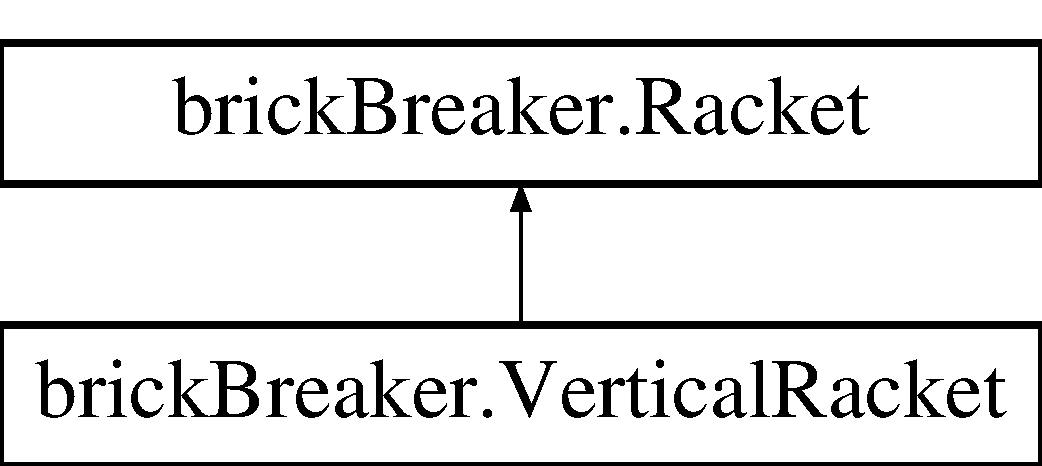
\includegraphics[height=2cm]{classbrick_breaker_1_1_vertical_racket}
\end{center}
\end{figure}
\subsection*{Public Member Functions}
\begin{DoxyCompactItemize}
\item 
\hyperlink{classbrick_breaker_1_1_vertical_racket_a2131363067760b416b9a857cba22c8ae}{VerticalRacket} (int arenaW, int arenaH, int racketW, boolean left)
\item 
void \hyperlink{classbrick_breaker_1_1_vertical_racket_ac455ce02602cbf621997042439809ee5}{draw} (Graphics g)
\item 
\hyperlink{classbrick_breaker_1_1_ball}{Ball} \hyperlink{classbrick_breaker_1_1_vertical_racket_a8893265e40d1d8946702d26f8c07887b}{checkCollision} (\hyperlink{classbrick_breaker_1_1_ball}{Ball} ball)
\item 
boolean \hyperlink{classbrick_breaker_1_1_vertical_racket_ac9edcb855d560fa5771da4e12abb4e71}{checkPast} (\hyperlink{classbrick_breaker_1_1_ball}{Ball} ball)
\item 
boolean \hyperlink{classbrick_breaker_1_1_vertical_racket_aa1af985933bd997bba1951e38107a5a5}{isLeft} ()
\item 
boolean \hyperlink{classbrick_breaker_1_1_vertical_racket_ad8c73b81712009be68fa497c48b71012}{isRight} ()
\end{DoxyCompactItemize}
\subsection*{Package Attributes}
\begin{DoxyCompactItemize}
\item 
\hypertarget{classbrick_breaker_1_1_vertical_racket_a044c4e4a5a331d2b51f1a4ee3d2e2b2e}{
boolean {\bfseries left}}
\label{classbrick_breaker_1_1_vertical_racket_a044c4e4a5a331d2b51f1a4ee3d2e2b2e}

\end{DoxyCompactItemize}


\subsection{Constructor \& Destructor Documentation}
\hypertarget{classbrick_breaker_1_1_vertical_racket_a2131363067760b416b9a857cba22c8ae}{
\index{brickBreaker::VerticalRacket@{brickBreaker::VerticalRacket}!VerticalRacket@{VerticalRacket}}
\index{VerticalRacket@{VerticalRacket}!brickBreaker::VerticalRacket@{brickBreaker::VerticalRacket}}
\subsubsection[{VerticalRacket}]{\setlength{\rightskip}{0pt plus 5cm}brickBreaker.VerticalRacket.VerticalRacket (int {\em arenaW}, \/  int {\em arenaH}, \/  int {\em racketW}, \/  boolean {\em left})}}
\label{classbrick_breaker_1_1_vertical_racket_a2131363067760b416b9a857cba22c8ae}
Constructor


\begin{DoxyParams}{Parameters}
\item[{\em arenaW}]The width of the screen on which play occurs \item[{\em arenaH}]The height of the screen on which play occurs \item[{\em racketW}]The width of the racket, in pixels \item[{\em left}]True if the racket is at the left side of the screen, false if it is at the right \end{DoxyParams}


\subsection{Member Function Documentation}
\hypertarget{classbrick_breaker_1_1_vertical_racket_a8893265e40d1d8946702d26f8c07887b}{
\index{brickBreaker::VerticalRacket@{brickBreaker::VerticalRacket}!checkCollision@{checkCollision}}
\index{checkCollision@{checkCollision}!brickBreaker::VerticalRacket@{brickBreaker::VerticalRacket}}
\subsubsection[{checkCollision}]{\setlength{\rightskip}{0pt plus 5cm}{\bf Ball} brickBreaker.VerticalRacket.checkCollision ({\bf Ball} {\em ball})\hspace{0.3cm}{\ttfamily  \mbox{[}virtual\mbox{]}}}}
\label{classbrick_breaker_1_1_vertical_racket_a8893265e40d1d8946702d26f8c07887b}
Checks if the ball collides with the racket and returns the updated ball


\begin{DoxyParams}{Parameters}
\item[{\em ball}]\hyperlink{classbrick_breaker_1_1_ball}{Ball} object to be tested \end{DoxyParams}
\begin{DoxyReturn}{Returns}
Returns the updated \hyperlink{classbrick_breaker_1_1_ball}{Ball} object 
\end{DoxyReturn}


Implements \hyperlink{classbrick_breaker_1_1_racket}{brickBreaker.Racket}.

\hypertarget{classbrick_breaker_1_1_vertical_racket_ac9edcb855d560fa5771da4e12abb4e71}{
\index{brickBreaker::VerticalRacket@{brickBreaker::VerticalRacket}!checkPast@{checkPast}}
\index{checkPast@{checkPast}!brickBreaker::VerticalRacket@{brickBreaker::VerticalRacket}}
\subsubsection[{checkPast}]{\setlength{\rightskip}{0pt plus 5cm}boolean brickBreaker.VerticalRacket.checkPast ({\bf Ball} {\em ball})\hspace{0.3cm}{\ttfamily  \mbox{[}virtual\mbox{]}}}}
\label{classbrick_breaker_1_1_vertical_racket_ac9edcb855d560fa5771da4e12abb4e71}
Checks if the ball is past the racket (and thus out of play)


\begin{DoxyParams}{Parameters}
\item[{\em ball}]\hyperlink{classbrick_breaker_1_1_ball}{Ball} to be tested \end{DoxyParams}
\begin{DoxyReturn}{Returns}
Returns true if the ball is past the racket, false if not 
\end{DoxyReturn}


Implements \hyperlink{classbrick_breaker_1_1_racket}{brickBreaker.Racket}.

\hypertarget{classbrick_breaker_1_1_vertical_racket_ac455ce02602cbf621997042439809ee5}{
\index{brickBreaker::VerticalRacket@{brickBreaker::VerticalRacket}!draw@{draw}}
\index{draw@{draw}!brickBreaker::VerticalRacket@{brickBreaker::VerticalRacket}}
\subsubsection[{draw}]{\setlength{\rightskip}{0pt plus 5cm}void brickBreaker.VerticalRacket.draw (Graphics {\em g})\hspace{0.3cm}{\ttfamily  \mbox{[}virtual\mbox{]}}}}
\label{classbrick_breaker_1_1_vertical_racket_ac455ce02602cbf621997042439809ee5}
Draws the racket on the screen.


\begin{DoxyParams}{Parameters}
\item[{\em g}]Graphics object used to draw \end{DoxyParams}


Implements \hyperlink{classbrick_breaker_1_1_racket}{brickBreaker.Racket}.

\hypertarget{classbrick_breaker_1_1_vertical_racket_aa1af985933bd997bba1951e38107a5a5}{
\index{brickBreaker::VerticalRacket@{brickBreaker::VerticalRacket}!isLeft@{isLeft}}
\index{isLeft@{isLeft}!brickBreaker::VerticalRacket@{brickBreaker::VerticalRacket}}
\subsubsection[{isLeft}]{\setlength{\rightskip}{0pt plus 5cm}boolean brickBreaker.VerticalRacket.isLeft ()}}
\label{classbrick_breaker_1_1_vertical_racket_aa1af985933bd997bba1951e38107a5a5}
Returns true if the racket is on the left side of the screen. 

Reimplemented from \hyperlink{classbrick_breaker_1_1_racket}{brickBreaker.Racket}.

\hypertarget{classbrick_breaker_1_1_vertical_racket_ad8c73b81712009be68fa497c48b71012}{
\index{brickBreaker::VerticalRacket@{brickBreaker::VerticalRacket}!isRight@{isRight}}
\index{isRight@{isRight}!brickBreaker::VerticalRacket@{brickBreaker::VerticalRacket}}
\subsubsection[{isRight}]{\setlength{\rightskip}{0pt plus 5cm}boolean brickBreaker.VerticalRacket.isRight ()}}
\label{classbrick_breaker_1_1_vertical_racket_ad8c73b81712009be68fa497c48b71012}
Returns true if the racket is on the right side of the screen. 

Reimplemented from \hyperlink{classbrick_breaker_1_1_racket}{brickBreaker.Racket}.



The documentation for this class was generated from the following file:\begin{DoxyCompactItemize}
\item 
game/brickBreaker/\hyperlink{_vertical_racket_8java}{VerticalRacket.java}\end{DoxyCompactItemize}

\hypertarget{classbrick_breaker_1_1web_1_1_web_config}{
\section{brickBreaker.web.WebConfig Class Reference}
\label{classbrick_breaker_1_1web_1_1_web_config}\index{brickBreaker::web::WebConfig@{brickBreaker::web::WebConfig}}
}
\subsection*{Public Types}
\begin{DoxyCompactItemize}
\item 
enum \hyperlink{classbrick_breaker_1_1web_1_1_web_config_a67fb01568cd83c5fa0685d95df6ca638}{Protocol} \{ {\bfseries HTTP} = ( \char`\"{}http\char`\"{} )
 \}
\end{DoxyCompactItemize}
\subsection*{Public Member Functions}
\begin{DoxyCompactItemize}
\item 
\hyperlink{classbrick_breaker_1_1web_1_1_web_config_a67fb01568cd83c5fa0685d95df6ca638}{Protocol} \hyperlink{classbrick_breaker_1_1web_1_1_web_config_a3718624e9a8e0cb7d4321cbadc716fae}{getProtocol} ()
\item 
void \hyperlink{classbrick_breaker_1_1web_1_1_web_config_acc5392f5644d6ca1a30736ca776a24eb}{setProtocol} (\hyperlink{classbrick_breaker_1_1web_1_1_web_config_a67fb01568cd83c5fa0685d95df6ca638}{Protocol} protocol)
\item 
String \hyperlink{classbrick_breaker_1_1web_1_1_web_config_a0face1c0ade730029ff6389b5a610112}{getHost} ()
\item 
void \hyperlink{classbrick_breaker_1_1web_1_1_web_config_a9746602db48181b7228b39c85bb7b34e}{setHost} (String host)
\item 
String \hyperlink{classbrick_breaker_1_1web_1_1_web_config_a2c7cb30ccc2b83bceada6faccc4f37fc}{getPath} ()
\item 
void \hyperlink{classbrick_breaker_1_1web_1_1_web_config_a3f4efd872b5cc690c9511a4d2e49ee89}{setPath} (String path)
\end{DoxyCompactItemize}
\subsection*{Static Public Member Functions}
\begin{DoxyCompactItemize}
\item 
static \hyperlink{classbrick_breaker_1_1web_1_1_web_config}{WebConfig} \hyperlink{classbrick_breaker_1_1web_1_1_web_config_aea2e81e51a4834d9d0bbc1705d7c4bfc}{getInstance} ()
\end{DoxyCompactItemize}


\subsection{Detailed Description}
This singleton class provides a centralized means of storing details about the remote server.

\begin{DoxyAuthor}{Author}
Abraham Lin 
\end{DoxyAuthor}


\subsection{Member Enumeration Documentation}
\hypertarget{classbrick_breaker_1_1web_1_1_web_config_a67fb01568cd83c5fa0685d95df6ca638}{
\index{brickBreaker::web::WebConfig@{brickBreaker::web::WebConfig}!Protocol@{Protocol}}
\index{Protocol@{Protocol}!brickBreaker::web::WebConfig@{brickBreaker::web::WebConfig}}
\subsubsection[{Protocol}]{\setlength{\rightskip}{0pt plus 5cm}enum {\bf brickBreaker::web::WebConfig::Protocol}}}
\label{classbrick_breaker_1_1web_1_1_web_config_a67fb01568cd83c5fa0685d95df6ca638}
This class enumerates all network protocols supported by the application.

\begin{DoxyAuthor}{Author}
Abraham Lin 
\end{DoxyAuthor}


\subsection{Member Function Documentation}
\hypertarget{classbrick_breaker_1_1web_1_1_web_config_a0face1c0ade730029ff6389b5a610112}{
\index{brickBreaker::web::WebConfig@{brickBreaker::web::WebConfig}!getHost@{getHost}}
\index{getHost@{getHost}!brickBreaker::web::WebConfig@{brickBreaker::web::WebConfig}}
\subsubsection[{getHost}]{\setlength{\rightskip}{0pt plus 5cm}String brickBreaker.web.WebConfig.getHost ()}}
\label{classbrick_breaker_1_1web_1_1_web_config_a0face1c0ade730029ff6389b5a610112}
Returns the hostname of the current remote server.

\begin{DoxyReturn}{Returns}
the hostname of the current remote server 
\end{DoxyReturn}
\hypertarget{classbrick_breaker_1_1web_1_1_web_config_aea2e81e51a4834d9d0bbc1705d7c4bfc}{
\index{brickBreaker::web::WebConfig@{brickBreaker::web::WebConfig}!getInstance@{getInstance}}
\index{getInstance@{getInstance}!brickBreaker::web::WebConfig@{brickBreaker::web::WebConfig}}
\subsubsection[{getInstance}]{\setlength{\rightskip}{0pt plus 5cm}static {\bf WebConfig} brickBreaker.web.WebConfig.getInstance ()\hspace{0.3cm}{\ttfamily  \mbox{[}static\mbox{]}}}}
\label{classbrick_breaker_1_1web_1_1_web_config_aea2e81e51a4834d9d0bbc1705d7c4bfc}
Returns this {\ttfamily \hyperlink{classbrick_breaker_1_1web_1_1_web_config}{WebConfig}}.

\begin{DoxyReturn}{Returns}
this {\ttfamily \hyperlink{classbrick_breaker_1_1web_1_1_web_config}{WebConfig}} 
\end{DoxyReturn}
\hypertarget{classbrick_breaker_1_1web_1_1_web_config_a2c7cb30ccc2b83bceada6faccc4f37fc}{
\index{brickBreaker::web::WebConfig@{brickBreaker::web::WebConfig}!getPath@{getPath}}
\index{getPath@{getPath}!brickBreaker::web::WebConfig@{brickBreaker::web::WebConfig}}
\subsubsection[{getPath}]{\setlength{\rightskip}{0pt plus 5cm}String brickBreaker.web.WebConfig.getPath ()}}
\label{classbrick_breaker_1_1web_1_1_web_config_a2c7cb30ccc2b83bceada6faccc4f37fc}
Returns the path to the application on the remote server.

\begin{DoxyReturn}{Returns}
the path 
\end{DoxyReturn}
\hypertarget{classbrick_breaker_1_1web_1_1_web_config_a3718624e9a8e0cb7d4321cbadc716fae}{
\index{brickBreaker::web::WebConfig@{brickBreaker::web::WebConfig}!getProtocol@{getProtocol}}
\index{getProtocol@{getProtocol}!brickBreaker::web::WebConfig@{brickBreaker::web::WebConfig}}
\subsubsection[{getProtocol}]{\setlength{\rightskip}{0pt plus 5cm}{\bf Protocol} brickBreaker.web.WebConfig.getProtocol ()}}
\label{classbrick_breaker_1_1web_1_1_web_config_a3718624e9a8e0cb7d4321cbadc716fae}
Returns the current network protocol used for accessing the remote server.

\begin{DoxyReturn}{Returns}
the current network protocol 
\end{DoxyReturn}
\hypertarget{classbrick_breaker_1_1web_1_1_web_config_a9746602db48181b7228b39c85bb7b34e}{
\index{brickBreaker::web::WebConfig@{brickBreaker::web::WebConfig}!setHost@{setHost}}
\index{setHost@{setHost}!brickBreaker::web::WebConfig@{brickBreaker::web::WebConfig}}
\subsubsection[{setHost}]{\setlength{\rightskip}{0pt plus 5cm}void brickBreaker.web.WebConfig.setHost (String {\em host})}}
\label{classbrick_breaker_1_1web_1_1_web_config_a9746602db48181b7228b39c85bb7b34e}
Sets the hostname of the remote server.


\begin{DoxyParams}{Parameters}
\item[{\em host}]the new hostname \end{DoxyParams}
\hypertarget{classbrick_breaker_1_1web_1_1_web_config_a3f4efd872b5cc690c9511a4d2e49ee89}{
\index{brickBreaker::web::WebConfig@{brickBreaker::web::WebConfig}!setPath@{setPath}}
\index{setPath@{setPath}!brickBreaker::web::WebConfig@{brickBreaker::web::WebConfig}}
\subsubsection[{setPath}]{\setlength{\rightskip}{0pt plus 5cm}void brickBreaker.web.WebConfig.setPath (String {\em path})}}
\label{classbrick_breaker_1_1web_1_1_web_config_a3f4efd872b5cc690c9511a4d2e49ee89}
Sets the path to the application on the remote server.


\begin{DoxyParams}{Parameters}
\item[{\em path}]the new path \end{DoxyParams}
\hypertarget{classbrick_breaker_1_1web_1_1_web_config_acc5392f5644d6ca1a30736ca776a24eb}{
\index{brickBreaker::web::WebConfig@{brickBreaker::web::WebConfig}!setProtocol@{setProtocol}}
\index{setProtocol@{setProtocol}!brickBreaker::web::WebConfig@{brickBreaker::web::WebConfig}}
\subsubsection[{setProtocol}]{\setlength{\rightskip}{0pt plus 5cm}void brickBreaker.web.WebConfig.setProtocol ({\bf Protocol} {\em protocol})}}
\label{classbrick_breaker_1_1web_1_1_web_config_acc5392f5644d6ca1a30736ca776a24eb}
Sets the network protocol used for accessing the remote server.


\begin{DoxyParams}{Parameters}
\item[{\em protocol}]the new network protocol \end{DoxyParams}


The documentation for this class was generated from the following file:\begin{DoxyCompactItemize}
\item 
src/game/brickBreaker/web/WebConfig.java\end{DoxyCompactItemize}

\hypertarget{classbrick_breaker_1_1web_1_1_web_exception}{
\section{brickBreaker.web.WebException Class Reference}
\label{classbrick_breaker_1_1web_1_1_web_exception}\index{brickBreaker::web::WebException@{brickBreaker::web::WebException}}
}
\subsection*{Public Member Functions}
\begin{DoxyCompactItemize}
\item 
\hyperlink{classbrick_breaker_1_1web_1_1_web_exception_a2f0867d6facf3647c37b8acf4bcef16a}{WebException} ()
\item 
\hyperlink{classbrick_breaker_1_1web_1_1_web_exception_af02e7ea5958f56cfe748bd6e332487e1}{WebException} (String message)
\item 
\hyperlink{classbrick_breaker_1_1web_1_1_web_exception_a2ef20379c84581f51570f9cae306a3f0}{WebException} (String message, Throwable cause)
\item 
\hyperlink{classbrick_breaker_1_1web_1_1_web_exception_a0fec67ad1b856715b5c5d9505fa65506}{WebException} (Throwable cause)
\end{DoxyCompactItemize}


\subsection{Detailed Description}
This class provides an application-\/specific wrapper for exceptions caused by failures to perform web-\/related functions.

\begin{DoxyAuthor}{Author}
Abraham Lin 
\end{DoxyAuthor}


\subsection{Constructor \& Destructor Documentation}
\hypertarget{classbrick_breaker_1_1web_1_1_web_exception_a2f0867d6facf3647c37b8acf4bcef16a}{
\index{brickBreaker::web::WebException@{brickBreaker::web::WebException}!WebException@{WebException}}
\index{WebException@{WebException}!brickBreaker::web::WebException@{brickBreaker::web::WebException}}
\subsubsection[{WebException}]{\setlength{\rightskip}{0pt plus 5cm}brickBreaker.web.WebException.WebException ()}}
\label{classbrick_breaker_1_1web_1_1_web_exception_a2f0867d6facf3647c37b8acf4bcef16a}
Constructs a new {\ttfamily \hyperlink{classbrick_breaker_1_1web_1_1_web_exception}{WebException}} with {\ttfamily null} as its detail message. \hypertarget{classbrick_breaker_1_1web_1_1_web_exception_af02e7ea5958f56cfe748bd6e332487e1}{
\index{brickBreaker::web::WebException@{brickBreaker::web::WebException}!WebException@{WebException}}
\index{WebException@{WebException}!brickBreaker::web::WebException@{brickBreaker::web::WebException}}
\subsubsection[{WebException}]{\setlength{\rightskip}{0pt plus 5cm}brickBreaker.web.WebException.WebException (String {\em message})}}
\label{classbrick_breaker_1_1web_1_1_web_exception_af02e7ea5958f56cfe748bd6e332487e1}
Constructs a new {\ttfamily \hyperlink{classbrick_breaker_1_1web_1_1_web_exception}{WebException}} with the specified detail message.


\begin{DoxyParams}{Parameters}
\item[{\em message}]the detail message \end{DoxyParams}
\hypertarget{classbrick_breaker_1_1web_1_1_web_exception_a2ef20379c84581f51570f9cae306a3f0}{
\index{brickBreaker::web::WebException@{brickBreaker::web::WebException}!WebException@{WebException}}
\index{WebException@{WebException}!brickBreaker::web::WebException@{brickBreaker::web::WebException}}
\subsubsection[{WebException}]{\setlength{\rightskip}{0pt plus 5cm}brickBreaker.web.WebException.WebException (String {\em message}, \/  Throwable {\em cause})}}
\label{classbrick_breaker_1_1web_1_1_web_exception_a2ef20379c84581f51570f9cae306a3f0}
Constructs a new {\ttfamily \hyperlink{classbrick_breaker_1_1web_1_1_web_exception}{WebException}} with the specified detail message and cause.


\begin{DoxyParams}{Parameters}
\item[{\em message}]the detail message \item[{\em cause}]the cause \end{DoxyParams}
\hypertarget{classbrick_breaker_1_1web_1_1_web_exception_a0fec67ad1b856715b5c5d9505fa65506}{
\index{brickBreaker::web::WebException@{brickBreaker::web::WebException}!WebException@{WebException}}
\index{WebException@{WebException}!brickBreaker::web::WebException@{brickBreaker::web::WebException}}
\subsubsection[{WebException}]{\setlength{\rightskip}{0pt plus 5cm}brickBreaker.web.WebException.WebException (Throwable {\em cause})}}
\label{classbrick_breaker_1_1web_1_1_web_exception_a0fec67ad1b856715b5c5d9505fa65506}
Constructs a new {\ttfamily \hyperlink{classbrick_breaker_1_1web_1_1_web_exception}{WebException}} with the specified cause.


\begin{DoxyParams}{Parameters}
\item[{\em cause}]the cause \end{DoxyParams}


The documentation for this class was generated from the following file:\begin{DoxyCompactItemize}
\item 
game/brickBreaker/web/WebException.java\end{DoxyCompactItemize}

\hypertarget{classbrick_breaker_1_1web_1_1_web_service}{
\section{brickBreaker.web.WebService Class Reference}
\label{classbrick_breaker_1_1web_1_1_web_service}\index{brickBreaker::web::WebService@{brickBreaker::web::WebService}}
}
\subsection*{Static Public Member Functions}
\begin{DoxyCompactItemize}
\item 
static boolean \hyperlink{classbrick_breaker_1_1web_1_1_web_service_a8643c4061b5d45c94fb04bd7f8e7a6c1}{verifyUser} (String username, String password)  throws WebException 
\item 
static List$<$ \hyperlink{classbrick_breaker_1_1web_1_1_online_level}{OnlineLevel} $>$ \hyperlink{classbrick_breaker_1_1web_1_1_web_service_af93134d4498f18f2483593520017f069}{getOnlineLevels} ()  throws WebException 
\item 
static \hyperlink{classbrick_breaker_1_1_level}{Level} \hyperlink{classbrick_breaker_1_1web_1_1_web_service_a7b62956bb6e061279fc3e3223a2b0d60}{downloadLevel} (String levelID)  throws WebException 
\item 
static void \hyperlink{classbrick_breaker_1_1web_1_1_web_service_ae6a847822ec25d4383104f83896c528d}{uploadLevel} (\hyperlink{classbrick_breaker_1_1_level}{Level} level, String title)  throws WebException 
\item 
static List$<$ \hyperlink{classbrick_breaker_1_1web_1_1_high_score}{HighScore} $>$ \hyperlink{classbrick_breaker_1_1web_1_1_web_service_a4dd0376683c3179b7bb6ff169833e5e6}{retrieveHighScores} (\hyperlink{classbrick_breaker_1_1_level}{Level} level)  throws WebException 
\item 
static void \hyperlink{classbrick_breaker_1_1web_1_1_web_service_a518c7c9660da1e22973ec62effaf6c70}{submitScore} (\hyperlink{classbrick_breaker_1_1_level}{Level} level, long score)  throws WebException 
\end{DoxyCompactItemize}


\subsection{Detailed Description}
This class provides web-\/based services for interacting with a remote server.

\begin{DoxyAuthor}{Author}
Abraham Lin 
\end{DoxyAuthor}


\subsection{Member Function Documentation}
\hypertarget{classbrick_breaker_1_1web_1_1_web_service_a7b62956bb6e061279fc3e3223a2b0d60}{
\index{brickBreaker::web::WebService@{brickBreaker::web::WebService}!downloadLevel@{downloadLevel}}
\index{downloadLevel@{downloadLevel}!brickBreaker::web::WebService@{brickBreaker::web::WebService}}
\subsubsection[{downloadLevel}]{\setlength{\rightskip}{0pt plus 5cm}static {\bf Level} brickBreaker.web.WebService.downloadLevel (String {\em levelID})  throws {\bf WebException} \hspace{0.3cm}{\ttfamily  \mbox{[}static\mbox{]}}}}
\label{classbrick_breaker_1_1web_1_1_web_service_a7b62956bb6e061279fc3e3223a2b0d60}
Downloads the level with the specified unique identifier.


\begin{DoxyParams}{Parameters}
\item[{\em levelID}]the unique identifier \end{DoxyParams}
\begin{DoxyReturn}{Returns}
the downloaded level
\end{DoxyReturn}

\begin{DoxyExceptions}{Exceptions}
\item[{\em \hyperlink{classbrick_breaker_1_1web_1_1_web_exception}{WebException}}]if any errors occur while attempting the operation \end{DoxyExceptions}
\hypertarget{classbrick_breaker_1_1web_1_1_web_service_af93134d4498f18f2483593520017f069}{
\index{brickBreaker::web::WebService@{brickBreaker::web::WebService}!getOnlineLevels@{getOnlineLevels}}
\index{getOnlineLevels@{getOnlineLevels}!brickBreaker::web::WebService@{brickBreaker::web::WebService}}
\subsubsection[{getOnlineLevels}]{\setlength{\rightskip}{0pt plus 5cm}static List$<${\bf OnlineLevel}$>$ brickBreaker.web.WebService.getOnlineLevels ()  throws {\bf WebException} \hspace{0.3cm}{\ttfamily  \mbox{[}static\mbox{]}}}}
\label{classbrick_breaker_1_1web_1_1_web_service_af93134d4498f18f2483593520017f069}
Returns a list of all levels available on the remote server.

\begin{DoxyReturn}{Returns}
the list of available levels
\end{DoxyReturn}

\begin{DoxyExceptions}{Exceptions}
\item[{\em \hyperlink{classbrick_breaker_1_1web_1_1_web_exception}{WebException}}]if any errors occur while attempting the operation \end{DoxyExceptions}
\hypertarget{classbrick_breaker_1_1web_1_1_web_service_a4dd0376683c3179b7bb6ff169833e5e6}{
\index{brickBreaker::web::WebService@{brickBreaker::web::WebService}!retrieveHighScores@{retrieveHighScores}}
\index{retrieveHighScores@{retrieveHighScores}!brickBreaker::web::WebService@{brickBreaker::web::WebService}}
\subsubsection[{retrieveHighScores}]{\setlength{\rightskip}{0pt plus 5cm}static List$<${\bf HighScore}$>$ brickBreaker.web.WebService.retrieveHighScores ({\bf Level} {\em level})  throws {\bf WebException} \hspace{0.3cm}{\ttfamily  \mbox{[}static\mbox{]}}}}
\label{classbrick_breaker_1_1web_1_1_web_service_a4dd0376683c3179b7bb6ff169833e5e6}
Retrieves high scores for the specified level from the remote server.


\begin{DoxyParams}{Parameters}
\item[{\em level}]the level \end{DoxyParams}
\begin{DoxyReturn}{Returns}
a list of high scores for that level retrieved from the remote server
\end{DoxyReturn}

\begin{DoxyExceptions}{Exceptions}
\item[{\em \hyperlink{classbrick_breaker_1_1web_1_1_web_exception}{WebException}}]if any errors occur while attempting the operation \end{DoxyExceptions}
\hypertarget{classbrick_breaker_1_1web_1_1_web_service_a518c7c9660da1e22973ec62effaf6c70}{
\index{brickBreaker::web::WebService@{brickBreaker::web::WebService}!submitScore@{submitScore}}
\index{submitScore@{submitScore}!brickBreaker::web::WebService@{brickBreaker::web::WebService}}
\subsubsection[{submitScore}]{\setlength{\rightskip}{0pt plus 5cm}static void brickBreaker.web.WebService.submitScore ({\bf Level} {\em level}, \/  long {\em score})  throws {\bf WebException} \hspace{0.3cm}{\ttfamily  \mbox{[}static\mbox{]}}}}
\label{classbrick_breaker_1_1web_1_1_web_service_a518c7c9660da1e22973ec62effaf6c70}
Submits a new high score to the remote server.


\begin{DoxyParams}{Parameters}
\item[{\em level}]the level with which the score is associated \item[{\em score}]the score\end{DoxyParams}

\begin{DoxyExceptions}{Exceptions}
\item[{\em \hyperlink{classbrick_breaker_1_1web_1_1_web_exception}{WebException}}]if any errors occur while attempting the operation \end{DoxyExceptions}
\hypertarget{classbrick_breaker_1_1web_1_1_web_service_ae6a847822ec25d4383104f83896c528d}{
\index{brickBreaker::web::WebService@{brickBreaker::web::WebService}!uploadLevel@{uploadLevel}}
\index{uploadLevel@{uploadLevel}!brickBreaker::web::WebService@{brickBreaker::web::WebService}}
\subsubsection[{uploadLevel}]{\setlength{\rightskip}{0pt plus 5cm}static void brickBreaker.web.WebService.uploadLevel ({\bf Level} {\em level}, \/  String {\em title})  throws {\bf WebException} \hspace{0.3cm}{\ttfamily  \mbox{[}static\mbox{]}}}}
\label{classbrick_breaker_1_1web_1_1_web_service_ae6a847822ec25d4383104f83896c528d}
Uploads a level to a remote server.


\begin{DoxyParams}{Parameters}
\item[{\em level}]the level to upload \item[{\em title}]the name for the level\end{DoxyParams}

\begin{DoxyExceptions}{Exceptions}
\item[{\em \hyperlink{classbrick_breaker_1_1web_1_1_web_exception}{WebException}}]if any errors occur while attempting the operation \end{DoxyExceptions}
\hypertarget{classbrick_breaker_1_1web_1_1_web_service_a8643c4061b5d45c94fb04bd7f8e7a6c1}{
\index{brickBreaker::web::WebService@{brickBreaker::web::WebService}!verifyUser@{verifyUser}}
\index{verifyUser@{verifyUser}!brickBreaker::web::WebService@{brickBreaker::web::WebService}}
\subsubsection[{verifyUser}]{\setlength{\rightskip}{0pt plus 5cm}static boolean brickBreaker.web.WebService.verifyUser (String {\em username}, \/  String {\em password})  throws {\bf WebException} \hspace{0.3cm}{\ttfamily  \mbox{[}static\mbox{]}}}}
\label{classbrick_breaker_1_1web_1_1_web_service_a8643c4061b5d45c94fb04bd7f8e7a6c1}
Returns whether the given login credentials are valid.


\begin{DoxyParams}{Parameters}
\item[{\em username}]the username \item[{\em password}]the password \end{DoxyParams}
\begin{DoxyReturn}{Returns}
whether the given username/password pair is valid
\end{DoxyReturn}

\begin{DoxyExceptions}{Exceptions}
\item[{\em \hyperlink{classbrick_breaker_1_1web_1_1_web_exception}{WebException}}]if any errors occur while attempting the operation \end{DoxyExceptions}


The documentation for this class was generated from the following file:\begin{DoxyCompactItemize}
\item 
game/brickBreaker/web/WebService.java\end{DoxyCompactItemize}

\hypertarget{classbrick_breaker_1_1web_1_1_x_m_l_parse_failure_exception}{
\section{brickBreaker.web.XMLParseFailureException Class Reference}
\label{classbrick_breaker_1_1web_1_1_x_m_l_parse_failure_exception}\index{brickBreaker::web::XMLParseFailureException@{brickBreaker::web::XMLParseFailureException}}
}
\subsection*{Public Member Functions}
\begin{DoxyCompactItemize}
\item 
\hyperlink{classbrick_breaker_1_1web_1_1_x_m_l_parse_failure_exception_a723d3ff61adb79b5cf401fe14c1832df}{XMLParseFailureException} ()
\item 
\hyperlink{classbrick_breaker_1_1web_1_1_x_m_l_parse_failure_exception_af66e18584855ce1dad5cc16b68ca7df1}{XMLParseFailureException} (String message)
\item 
\hyperlink{classbrick_breaker_1_1web_1_1_x_m_l_parse_failure_exception_a481f9e2823e591526dddb632a3cb8ab7}{XMLParseFailureException} (String message, Throwable cause)
\item 
\hyperlink{classbrick_breaker_1_1web_1_1_x_m_l_parse_failure_exception_aa07904b5ff321a28d6ed9669236fa98b}{XMLParseFailureException} (Throwable cause)
\end{DoxyCompactItemize}


\subsection{Detailed Description}
This class provides an application-\/specific wrapper for exceptions caused by a failure to parse string representations of XML.

\begin{DoxyAuthor}{Author}
Abraham Lin 
\end{DoxyAuthor}


\subsection{Constructor \& Destructor Documentation}
\hypertarget{classbrick_breaker_1_1web_1_1_x_m_l_parse_failure_exception_a723d3ff61adb79b5cf401fe14c1832df}{
\index{brickBreaker::web::XMLParseFailureException@{brickBreaker::web::XMLParseFailureException}!XMLParseFailureException@{XMLParseFailureException}}
\index{XMLParseFailureException@{XMLParseFailureException}!brickBreaker::web::XMLParseFailureException@{brickBreaker::web::XMLParseFailureException}}
\subsubsection[{XMLParseFailureException}]{\setlength{\rightskip}{0pt plus 5cm}brickBreaker.web.XMLParseFailureException.XMLParseFailureException ()}}
\label{classbrick_breaker_1_1web_1_1_x_m_l_parse_failure_exception_a723d3ff61adb79b5cf401fe14c1832df}
Constructs a new {\ttfamily \hyperlink{classbrick_breaker_1_1web_1_1_x_m_l_parse_failure_exception}{XMLParseFailureException}} with {\ttfamily null} as its detail message. \hypertarget{classbrick_breaker_1_1web_1_1_x_m_l_parse_failure_exception_af66e18584855ce1dad5cc16b68ca7df1}{
\index{brickBreaker::web::XMLParseFailureException@{brickBreaker::web::XMLParseFailureException}!XMLParseFailureException@{XMLParseFailureException}}
\index{XMLParseFailureException@{XMLParseFailureException}!brickBreaker::web::XMLParseFailureException@{brickBreaker::web::XMLParseFailureException}}
\subsubsection[{XMLParseFailureException}]{\setlength{\rightskip}{0pt plus 5cm}brickBreaker.web.XMLParseFailureException.XMLParseFailureException (String {\em message})}}
\label{classbrick_breaker_1_1web_1_1_x_m_l_parse_failure_exception_af66e18584855ce1dad5cc16b68ca7df1}
Constructs a new {\ttfamily \hyperlink{classbrick_breaker_1_1web_1_1_x_m_l_parse_failure_exception}{XMLParseFailureException}} with the specified detail message.


\begin{DoxyParams}{Parameters}
\item[{\em message}]the detail message \end{DoxyParams}
\hypertarget{classbrick_breaker_1_1web_1_1_x_m_l_parse_failure_exception_a481f9e2823e591526dddb632a3cb8ab7}{
\index{brickBreaker::web::XMLParseFailureException@{brickBreaker::web::XMLParseFailureException}!XMLParseFailureException@{XMLParseFailureException}}
\index{XMLParseFailureException@{XMLParseFailureException}!brickBreaker::web::XMLParseFailureException@{brickBreaker::web::XMLParseFailureException}}
\subsubsection[{XMLParseFailureException}]{\setlength{\rightskip}{0pt plus 5cm}brickBreaker.web.XMLParseFailureException.XMLParseFailureException (String {\em message}, \/  Throwable {\em cause})}}
\label{classbrick_breaker_1_1web_1_1_x_m_l_parse_failure_exception_a481f9e2823e591526dddb632a3cb8ab7}
Constructs a new {\ttfamily \hyperlink{classbrick_breaker_1_1web_1_1_x_m_l_parse_failure_exception}{XMLParseFailureException}} with the specified detail message and cause.


\begin{DoxyParams}{Parameters}
\item[{\em message}]the detail message \item[{\em cause}]the cause \end{DoxyParams}
\hypertarget{classbrick_breaker_1_1web_1_1_x_m_l_parse_failure_exception_aa07904b5ff321a28d6ed9669236fa98b}{
\index{brickBreaker::web::XMLParseFailureException@{brickBreaker::web::XMLParseFailureException}!XMLParseFailureException@{XMLParseFailureException}}
\index{XMLParseFailureException@{XMLParseFailureException}!brickBreaker::web::XMLParseFailureException@{brickBreaker::web::XMLParseFailureException}}
\subsubsection[{XMLParseFailureException}]{\setlength{\rightskip}{0pt plus 5cm}brickBreaker.web.XMLParseFailureException.XMLParseFailureException (Throwable {\em cause})}}
\label{classbrick_breaker_1_1web_1_1_x_m_l_parse_failure_exception_aa07904b5ff321a28d6ed9669236fa98b}
Constructs a new {\ttfamily \hyperlink{classbrick_breaker_1_1web_1_1_x_m_l_parse_failure_exception}{XMLParseFailureException}} with the specified cause.


\begin{DoxyParams}{Parameters}
\item[{\em cause}]the cause \end{DoxyParams}


The documentation for this class was generated from the following file:\begin{DoxyCompactItemize}
\item 
game/brickBreaker/web/XMLParseFailureException.java\end{DoxyCompactItemize}

\hypertarget{classbrick_breaker_1_1web_1_1_x_m_l_util}{
\section{brickBreaker.web.XMLUtil Class Reference}
\label{classbrick_breaker_1_1web_1_1_x_m_l_util}\index{brickBreaker::web::XMLUtil@{brickBreaker::web::XMLUtil}}
}
\subsection*{Static Public Member Functions}
\begin{DoxyCompactItemize}
\item 
static Document \hyperlink{classbrick_breaker_1_1web_1_1_x_m_l_util_a0a68ec3df3895e11d5c847f68af7953f}{parseXML} (String xmlString)  throws XMLParseFailureException 
\end{DoxyCompactItemize}


\subsection{Detailed Description}
This class provides methods for manipulating XML documents.

\begin{DoxyAuthor}{Author}
Abraham Lin 
\end{DoxyAuthor}


\subsection{Member Function Documentation}
\hypertarget{classbrick_breaker_1_1web_1_1_x_m_l_util_a0a68ec3df3895e11d5c847f68af7953f}{
\index{brickBreaker::web::XMLUtil@{brickBreaker::web::XMLUtil}!parseXML@{parseXML}}
\index{parseXML@{parseXML}!brickBreaker::web::XMLUtil@{brickBreaker::web::XMLUtil}}
\subsubsection[{parseXML}]{\setlength{\rightskip}{0pt plus 5cm}static Document brickBreaker.web.XMLUtil.parseXML (String {\em xmlString})  throws {\bf XMLParseFailureException} \hspace{0.3cm}{\ttfamily  \mbox{[}static\mbox{]}}}}
\label{classbrick_breaker_1_1web_1_1_x_m_l_util_a0a68ec3df3895e11d5c847f68af7953f}
Parses an XML string into an XML document.


\begin{DoxyParams}{Parameters}
\item[{\em xmlString}]the XML document in {\ttfamily String} form \end{DoxyParams}
\begin{DoxyReturn}{Returns}
the XML document in {\ttfamily Document} form
\end{DoxyReturn}

\begin{DoxyExceptions}{Exceptions}
\item[{\em \hyperlink{classbrick_breaker_1_1web_1_1_x_m_l_parse_failure_exception}{XMLParseFailureException}}]if any errors occur while attempting the encryption process \end{DoxyExceptions}


The documentation for this class was generated from the following file:\begin{DoxyCompactItemize}
\item 
src/game/brickBreaker/web/XMLUtil.java\end{DoxyCompactItemize}

\chapter{File Documentation}
\hypertarget{_ball_8java}{
\section{game/brickBreaker/Ball.java File Reference}
\label{_ball_8java}\index{game/brickBreaker/Ball.java@{game/brickBreaker/Ball.java}}
}
\subsection*{Classes}
\begin{DoxyCompactItemize}
\item 
class \hyperlink{classbrick_breaker_1_1_ball}{brickBreaker.Ball}
\end{DoxyCompactItemize}


\subsection{Detailed Description}
Represents a ball object, which bounces around the screen bouncing off walls, bricks and rackets.

\begin{DoxyAuthor}{Author}
Jacob Pritt 
\end{DoxyAuthor}
\begin{DoxyVersion}{Version}
4/30/10 
\end{DoxyVersion}

\hypertarget{_brick_8java}{
\section{game/brickBreaker/Brick.java File Reference}
\label{_brick_8java}\index{game/brickBreaker/Brick.java@{game/brickBreaker/Brick.java}}
}
\subsection*{Classes}
\begin{DoxyCompactItemize}
\item 
class \hyperlink{classbrick_breaker_1_1_brick}{brickBreaker.Brick}
\end{DoxyCompactItemize}


\subsection{Detailed Description}
Abstract class Brick -\/ represents a brick object on the screen

\begin{DoxyAuthor}{Author}
Jacob Pritt 
\end{DoxyAuthor}
\begin{DoxyVersion}{Version}
4/30/10
\end{DoxyVersion}
\begin{DoxySeeAlso}{See also}
\hyperlink{_standard_brick_8java}{StandardBrick.java}, \hyperlink{_power_brick_8java}{PowerBrick.java}, \hyperlink{_permanent_brick_8java}{PermanentBrick.java} 
\end{DoxySeeAlso}

\hypertarget{_game_panel_8java}{
\section{src/game/brickBreaker/GamePanel.java File Reference}
\label{_game_panel_8java}\index{src/game/brickBreaker/GamePanel.java@{src/game/brickBreaker/GamePanel.java}}
}
\subsection*{Classes}
\begin{DoxyCompactItemize}
\item 
class \hyperlink{classbrick_breaker_1_1_game_panel}{brickBreaker.GamePanel}
\end{DoxyCompactItemize}


\subsection{Detailed Description}
Creates a panel that controls and displays game play.

\begin{DoxyAuthor}{Author}
Jacob Pritt 
\end{DoxyAuthor}
\begin{DoxyVersion}{Version}
4/30/10 
\end{DoxyVersion}

\hypertarget{_horizontal_racket_8java}{
\section{src/game/brickBreaker/HorizontalRacket.java File Reference}
\label{_horizontal_racket_8java}\index{src/game/brickBreaker/HorizontalRacket.java@{src/game/brickBreaker/HorizontalRacket.java}}
}
\subsection*{Classes}
\begin{DoxyCompactItemize}
\item 
class \hyperlink{classbrick_breaker_1_1_horizontal_racket}{brickBreaker.HorizontalRacket}
\end{DoxyCompactItemize}


\subsection{Detailed Description}
Represents a racket that moves horizontally, either at the top or bottom of the screen. See class Racket for more information.

\begin{DoxyAuthor}{Author}
Jacob Pritt 
\end{DoxyAuthor}
\begin{DoxyVersion}{Version}
4/30/10
\end{DoxyVersion}
\begin{DoxySeeAlso}{See also}
\hyperlink{_racket_8java}{Racket.java} 
\end{DoxySeeAlso}

\hypertarget{_idle_panel_8java}{
\section{src/game/brickBreaker/IdlePanel.java File Reference}
\label{_idle_panel_8java}\index{src/game/brickBreaker/IdlePanel.java@{src/game/brickBreaker/IdlePanel.java}}
}
\subsection*{Classes}
\begin{DoxyCompactItemize}
\item 
class \hyperlink{classbrick_breaker_1_1_idle_panel}{brickBreaker.IdlePanel}
\end{DoxyCompactItemize}


\subsection{Detailed Description}
class IdlePanel -\/ This is the panel from which the user can enter a game, the level editor, or interact with the online database.

\begin{DoxyAuthor}{Author}
Robert Nishihara 
\end{DoxyAuthor}
\begin{DoxyVersion}{Version}
5/02/10 
\end{DoxyVersion}

\hypertarget{_level_8java}{
\section{src/game/brickBreaker/Level.java File Reference}
\label{_level_8java}\index{src/game/brickBreaker/Level.java@{src/game/brickBreaker/Level.java}}
}
\subsection*{Classes}
\begin{DoxyCompactItemize}
\item 
class \hyperlink{classbrick_breaker_1_1_level}{brickBreaker.Level}
\end{DoxyCompactItemize}


\subsection{Detailed Description}
Contains all of the data necessary to initialize a level. This object is passed to LevelPlayer to play a level.

\begin{DoxyAuthor}{Author}
Jacob Pritt 
\end{DoxyAuthor}
\begin{DoxyVersion}{Version}
4/30/10
\end{DoxyVersion}
\begin{DoxySeeAlso}{See also}
\hyperlink{_level_player_8java}{LevelPlayer.java} 
\end{DoxySeeAlso}

\hypertarget{_level_player_8java}{
\section{src/game/brickBreaker/LevelPlayer.java File Reference}
\label{_level_player_8java}\index{src/game/brickBreaker/LevelPlayer.java@{src/game/brickBreaker/LevelPlayer.java}}
}
\subsection*{Classes}
\begin{DoxyCompactItemize}
\item 
class \hyperlink{classbrick_breaker_1_1_level_player}{brickBreaker.LevelPlayer}
\end{DoxyCompactItemize}


\subsection{Detailed Description}
Controls the updating and interation of different components in a Level object.

\begin{DoxyAuthor}{Author}
Jacob Pritt 
\end{DoxyAuthor}
\begin{DoxyVersion}{Version}
4/30/10
\end{DoxyVersion}
\begin{DoxySeeAlso}{See also}
\hyperlink{_level_8java}{Level.java} 
\end{DoxySeeAlso}

\hypertarget{_password_box_8java}{
\section{src/game/brickBreaker/PasswordBox.java File Reference}
\label{_password_box_8java}\index{src/game/brickBreaker/PasswordBox.java@{src/game/brickBreaker/PasswordBox.java}}
}
\subsection*{Classes}
\begin{DoxyCompactItemize}
\item 
class \hyperlink{classbrick_breaker_1_1_password_box}{brickBreaker.PasswordBox}
\end{DoxyCompactItemize}


\subsection{Detailed Description}
Initializes a panel with a username and password prompt, with the option to skip login.

\begin{DoxyAuthor}{Author}
Jacob Pritt 
\end{DoxyAuthor}
\begin{DoxyVersion}{Version}
4/30/10 
\end{DoxyVersion}

\hypertarget{_permanent_brick_8java}{
\section{game/brickBreaker/PermanentBrick.java File Reference}
\label{_permanent_brick_8java}\index{game/brickBreaker/PermanentBrick.java@{game/brickBreaker/PermanentBrick.java}}
}
\subsection*{Classes}
\begin{DoxyCompactItemize}
\item 
class \hyperlink{classbrick_breaker_1_1_permanent_brick}{brickBreaker.PermanentBrick}
\end{DoxyCompactItemize}


\subsection{Detailed Description}
Represents a permanent brick object, which can never be removed.

\begin{DoxyAuthor}{Author}
Jacob Pritt 
\end{DoxyAuthor}
\begin{DoxyVersion}{Version}
4/30/10
\end{DoxyVersion}
\begin{DoxySeeAlso}{See also}
\hyperlink{_brick_8java}{Brick.java} 
\end{DoxySeeAlso}

\hypertarget{_power_brick_8java}{
\section{game/brickBreaker/PowerBrick.java File Reference}
\label{_power_brick_8java}\index{game/brickBreaker/PowerBrick.java@{game/brickBreaker/PowerBrick.java}}
}
\subsection*{Classes}
\begin{DoxyCompactItemize}
\item 
class \hyperlink{classbrick_breaker_1_1_power_brick}{brickBreaker.PowerBrick}
\end{DoxyCompactItemize}


\subsection{Detailed Description}
Represents a brick that offers a \char`\"{}Power Up\char`\"{} when it is hit by a ball, increasing game speed, point multipliers, etc.

\begin{DoxyAuthor}{Author}
Jacob Pritt 
\end{DoxyAuthor}
\begin{DoxyVersion}{Version}
4/30/10
\end{DoxyVersion}
\begin{DoxySeeAlso}{See also}
\hyperlink{_brick_8java}{Brick.java} 
\end{DoxySeeAlso}

\hypertarget{_p_r_panel_8java}{
\section{src/game/brickBreaker/PRPanel.java File Reference}
\label{_p_r_panel_8java}\index{src/game/brickBreaker/PRPanel.java@{src/game/brickBreaker/PRPanel.java}}
}
\subsection*{Classes}
\begin{DoxyCompactItemize}
\item 
class \hyperlink{classbrick_breaker_1_1_p_r_panel}{brickBreaker.PRPanel}
\end{DoxyCompactItemize}


\subsection{Detailed Description}
PRPanel is an extension of the JPanel class that includes pause(), resume(), start() and stop() methods

\begin{DoxyAuthor}{Author}
Jacob Pritt 
\end{DoxyAuthor}
\begin{DoxyVersion}{Version}
4/30/10 
\end{DoxyVersion}

\hypertarget{_racket_8java}{
\section{src/game/brickBreaker/Racket.java File Reference}
\label{_racket_8java}\index{src/game/brickBreaker/Racket.java@{src/game/brickBreaker/Racket.java}}
}
\subsection*{Classes}
\begin{DoxyCompactItemize}
\item 
class \hyperlink{classbrick_breaker_1_1_racket}{brickBreaker.Racket}
\end{DoxyCompactItemize}


\subsection{Detailed Description}
Represents a racket on one side of the screen, controlled by the user to keep the ball in the air.

\begin{DoxyAuthor}{Author}
Jacob Pritt 
\end{DoxyAuthor}
\begin{DoxyVersion}{Version}
4/30/10
\end{DoxyVersion}
\begin{DoxySeeAlso}{See also}
\hyperlink{_horizontal_racket_8java}{HorizontalRacket.java}, \hyperlink{_vertical_racket_8java}{VerticalRacket.java} 
\end{DoxySeeAlso}

\hypertarget{_standard_brick_8java}{
\section{game/brickBreaker/StandardBrick.java File Reference}
\label{_standard_brick_8java}\index{game/brickBreaker/StandardBrick.java@{game/brickBreaker/StandardBrick.java}}
}
\subsection*{Classes}
\begin{DoxyCompactItemize}
\item 
class \hyperlink{classbrick_breaker_1_1_standard_brick}{brickBreaker.StandardBrick}
\end{DoxyCompactItemize}


\subsection{Detailed Description}
Represents the StandardBrick object used in the game.

\begin{DoxyAuthor}{Author}
Jacob Pritt 
\end{DoxyAuthor}
\begin{DoxyVersion}{Version}
4/30/10
\end{DoxyVersion}
\begin{DoxySeeAlso}{See also}
\hyperlink{_brick_8java}{Brick.java} 
\end{DoxySeeAlso}

\hypertarget{_start_8java}{
\section{src/game/brickBreaker/Start.java File Reference}
\label{_start_8java}\index{src/game/brickBreaker/Start.java@{src/game/brickBreaker/Start.java}}
}
\subsection*{Classes}
\begin{DoxyCompactItemize}
\item 
class \hyperlink{classbrick_breaker_1_1_start}{brickBreaker.Start}
\end{DoxyCompactItemize}


\subsection{Detailed Description}
The overarching JFrame which contains and controls the panels used for game play and level editing.

\begin{DoxyAuthor}{Author}
Jacob Pritt 
\end{DoxyAuthor}
\begin{DoxyVersion}{Version}
4/30/10 
\end{DoxyVersion}

\hypertarget{_vertical_racket_8java}{
\section{src/game/brickBreaker/VerticalRacket.java File Reference}
\label{_vertical_racket_8java}\index{src/game/brickBreaker/VerticalRacket.java@{src/game/brickBreaker/VerticalRacket.java}}
}
\subsection*{Classes}
\begin{DoxyCompactItemize}
\item 
class \hyperlink{classbrick_breaker_1_1_vertical_racket}{brickBreaker.VerticalRacket}
\end{DoxyCompactItemize}


\subsection{Detailed Description}
Represents a racket that moves vertically, either at the right or left side of the screen. See class Racket for more information.

\begin{DoxyAuthor}{Author}
Jacob Pritt 
\end{DoxyAuthor}
\begin{DoxyVersion}{Version}
4/30/10
\end{DoxyVersion}
\begin{DoxySeeAlso}{See also}
\hyperlink{_racket_8java}{Racket.java} 
\end{DoxySeeAlso}

\printindex
\end{document}
